\documentclass[xcolor={table}]{beamer}
\usepackage{fleqn}
%\usepackage{epsf}
\usepackage{graphicx}
\usepackage{coordsys} %for \numbline command
%\usepackage{dingbat}
%\usepackage{aima2e-slides}

%Setup appearance:

\usetheme{Darmstadt}
%\usefonttheme[onlylarge]{structurebold}
\usefonttheme{professionalfonts} %this ensures beamer doesn't mess up the \hat and \tilde commands
\setbeamerfont*{frametitle}{size=\normalsize,series=\bfseries}
\setbeamertemplate{navigation symbols}{}
\setbeamertemplate{bibliography item}{[\theenumiv]}
\setbeamertemplate{caption}[numbered]

% Standard packages
\usepackage[english]{babel}
\usepackage[latin1]{inputenc}
\usepackage{times}
\usepackage[T1]{fontenc}
\usepackage{multirow}
\usepackage{subfigure}
\usepackage{pbox}
\usepackage{arydshln}
\usepackage{pifont}
\usepackage{cancel}

% Source Code packages
%\usepackage{algorithmicx}
\usepackage{algorithm}
\usepackage{algpseudocode}
\algrenewcommand\alglinenumber[1]{\tiny #1:} %make the line number size in the algorithmicx algorithm environment (which is loaded by algpseudocode smaller
%\algsetup{linenosize=\tiny}
%\usepackage{algorithm2e}
% to correct indentation in algorithmic environments
% https://www.latex4technics.com/?note=wwr
%\newcommand{\algmargin}{\the\ALG@thistlm}
%\makeatother
%\newlength{\whilewidth}
%\settowidth{\whilewidth}{\algorithmicwhile\ }
%\algdef{SE}[parWHILE]{parWhile}{EndparWhile}[1]
%  {\parbox[t]{\dimexpr\linewidth-\algmargin}{%
%     \hangindent\whilewidth\strut\algorithmicwhile\ #1\ \algorithmicdo\strut}}{\algorithmicend\ \algorithmicwhile}
%\algnewcommand{\parState}[1]{\State%
%  \parbox[t]{\dimexpr\linewidth-\algmargin}{\strut #1\strut}}

\usepackage{listings}

\lstset{ %
language=Octave,                % choose the language of the code
basicstyle=\footnotesize,       % the size of the fonts that are used for the code
numbers=left,                   % where to put the line-numbers
numberstyle=\footnotesize,      % the size of the fonts that are used for the line-numbers
stepnumber=1,                   % the step between two line-numbers. If it's 1 each line will be numbered
numbersep=5pt,                  % how far the line-numbers are from the code
backgroundcolor=\color{white},  % choose the background color. You must add \usepackage{color}
showspaces=false,               % show spaces adding particular underscores
showstringspaces=false,         % underline spaces within strings
showtabs=false,                 % show tabs within strings adding particular underscores
frame=single,	                % adds a frame around the code
tabsize=2,	                % sets default tabsize to 2 spaces
captionpos=b,                   % sets the caption-position to bottom
breaklines=true,                % sets automatic line breaking
breakatwhitespace=false,        % sets if automatic breaks should only happen at whitespace
escapeinside={\%*}{*)}          % if you want to add a comment within your code
}

% Setup TikZ
\usepackage{tikz}
\usetikzlibrary{arrows}
\tikzstyle{block}=[draw opacity=0.7,line width=1.4cm]

%%%%%%%%%%%%%%%%%%%%%%%%%%%%%%%%%%%%%%%%%%%%
%% Start newcommand defs taken from aima slides style file %%%%%%%%%%%%%%
%%%%%%%%%%%%%%%%%%%%%%%%%%%%%%%%%%%%%%%%%%%%

%%%%%%%%%%%% elements of programs %%%%%%%%%%%%%%%%%%%%%%%%%%%%%%%%%


\newlength{\codewidth}
\setlength{\codewidth}{\textwidth}
\addtolength{\codewidth}{-0.5in}

\newcommand{\FigBox}[1]{%%% The alternative to figbox - pnorvig
\noindent\framebox[\textwidth]{%
\begin{minipage}{\codewidth}%
#1%
\end{minipage}}%
}

\newcommand{\defprog}[1]{\txr{\mbox{{\sc #1}}}}
\newcommand{\prog}[1]{\mbox{{\sc #1}}}   %%% same as defprog
\newcommand{\noprog}[1]{\mbox{{\sc #1}}} %%% same as defprog
\newcommand{\system}[1]{\mbox{{\sc #1}}} %%% same as defprog
\newcommand{\nosystem}[1]{\mbox{{\sc #1}}} %%% same as defprog
\newcommand{\act}[1]{{\it #1}}
\newcommand{\key}[1]{\txb{{\bf #1}}}
\def\k{\key}
\newcommand{\var}[1]{\txg{{\it #1}}}
\def\v{\var}
\def\p{\prg}
\newcommand{\setq}[2]{#1\hbox{$\,\leftarrow\,$}#2}
\newcommand{\setqmath}[2]{#1 \leftarrow #2}

%%pnorvig Mar 14 1994:
\newcommand{\labl}[1]{\prog{#1}}	% Statement Label in code
\newcommand{\cmt}[1]{{\tt /*} {\it #1} {\tt */}}	% Comment in code
\newcommand{\rcmt}[1]{\hfill {\tt /*} {\it #1} {\tt */}}
\newcommand{\Endfn}[1]{}		% End of a function in code
\newcommand{\fnsep}{\hspace*{0in}\raisebox{3pt}{\rule{\codewidth}{0.2pt}}\hfill}	% Between functions in code

\def\code{\noindent\nobreak\begin{scriptsize}
        \begingroup\obeylines\obeyspaces\docode}
\def\docode#1{\noindent\framebox[\columnwidth][l]%
{~~\begin{minipage}{\codewidth}~
#1
~\end{minipage}}\endgroup%
\nobreak\end{scriptsize}\noindent\ignorespaces}
\def\asis{\obeylines\obeyspaces}
\def\ttp{.\skip -0.5em\ }
{\obeyspaces\global\def {\ }}

%% Fine tuning for perfect formatting

\newcommand{\ac}{,\hspace{0.15em}}
\newcommand{\ts}{\,}
\newcommand{\bodysep}{\vspace{0.1in}}
\newcommand{\subfnsep}{\vspace{0.06in}}
\newcommand{\prebnfsep}{\vspace{-0.25in}}
\newcommand{\postbnfsep}{\vspace{0.1in}}
\newcommand{\fnvar}[1]{\prog{#1}}
\newcommand{\func}[3]{\key{function} \defprog{#1}(\txg{#2}) \key{returns} #3}
\newcommand{\nofunc}[3]{\key{function} \noprog{#1}(#2) \key{returns} #3}
\newcommand{\proc}[2]{\key{procedure} \defprog{#1}(\txg{#2})}
\newcommand{\noproc}[2]{\key{procedure} \noprog{#1}(#2)}
\newcommand{\firstinputs}[2]{\key{inputs}: \var{#1}, #2}
\newcommand{\inputs}[2]{\phantom{\key{inputs}: }\var{#1}, #2}
\newcommand{\firstlocal}[2]{\key{local variables}: \var{#1}, #2}
\newcommand{\local}[2]{\phantom{\key{local variables}: }\var{#1}, #2}
\newcommand{\firststatic}[2]{\key{static}: \var{#1}, #2}
\newcommand{\static}[2]{\phantom{\key{static}: }\var{#1}, #2}

%%%%%%%%%%%%%%%%%%%%%%%%%%

\def\mysum{\begin{Huge}\mbox{$\Sigma$}\end{Huge}}
\def\myint{\begin{LARGE}\mbox{$\int$}\end{LARGE}}
\def\myprod{\begin{Huge}\mbox{$\Pi$}\end{Huge}}

\font\smathbold=cmbx10 scaled 1700
\newcommand{\smbf}[1]{\mbox{{\smathbold #1}}}
\newcommand{\mbf}[1]{\mbox{{\bf #1}}}

%%%%%%% Useful formatting commands for lines of text etc.
\def\tab{\hbox{\kern0.4in}}    %% Insert space (even at start of line)
\def\al{\\\tab}                %% Next line is indented
\def\nl{\\\tab\tab}            %% Next line is double-indented
\def\nnl{\\\tab\tab\tab}       %% Next line is triple-indented
%\def{$\diamondsuit\ \ $}  %% Itemization without all the spacing
\def\bull{\vskip -8pt\item{$\bullet$\ }} %% Itemization with less spacing
\def\u#1{$\underline{\mbox{#1}}$}
\def\q#1{\txm{\u{#1}??}}

%%%%%% logical symbols
\newcommand{\entails}{\models}
%\newcommand{\implies}{\:\;{\Rightarrow}\:\;}
\newcommand{\textimplies}{\;{\Rightarrow}\;}
\newcommand{\impliessymbol}{\Rightarrow}
\newcommand{\lequiv}{\;\;{\Leftrightarrow}\;\;}
\newcommand{\textlequiv}{\;{\Leftrightarrow}\;}
\newcommand{\lequivsymbol}{\Leftrightarrow}
\newcommand{\xor}{\not\lequiv}
\newcommand{\All}[1]{\forall\,#1\;\;}
\newcommand{\Exi}[1]{\exists\,#1\;\;}
\newcommand{\Exii}[1]{\exists!\,#1\;\;}% -pnorvig
\newcommand{\Iot}[2]{\iota\,#1\,#2}
\newcommand{\Lam}[2]{\lambda #1\;#2}
\newcommand{\Qua}[3]{[#1\,#2\;#3]}

\newcommand{\union}{{\,{\cup}\,}}
\newcommand{\intersection}{{\,{\cap}\,}}
\renewcommand{\emptyset}{\{\,\}}
\newcommand{\emptylist}{[\,]}
\newcommand{\adjoin}[2]{\{#1|#2\}}
\newcommand{\elt}{{\,{\in}\,}}  %%%cuts down on spacing
\newcommand{\eq}{{\,{=}\,}}  %%%cuts down on spacing
\def\stimes{{\,\times\,}}       %%%cuts down on spacing


%%%%%%% Formatting tables - AIMA uses full-width tables with spacing

\newenvironment{mytabular}%
{\noindent\begin{tabular*}{\textwidth}}%
{\end{tabular*}}

\newcommand{\tabtop}{\rule{0pt}{2ex}}%%Use after hline in body of table
\newcommand{\tabbot}{\rule[-1ex]{0pt}{1.8ex}}%%Use before hline " " " "
\newcommand{\tabhead}{\rule[-0.85ex]{0pt}{2.8ex}}%%Use in lines between hlines
\newcommand{\squad}{\hspace*{0.5em}}%%Use occasionally at left edge
\newcommand{\sq}[1]{\hspace*{#1\textwidth}}
\def\tf{\rm} %% table font


\def\<{\langle}
\def\>{\rangle}

%\usepackage[dvips]{color}
\definecolor{myred}{rgb}{0.7,0.0,0.0}
\definecolor{myblue}{rgb}{0.0,0.0,0.5}
\definecolor{mygreen}{rgb}{0.0,0.3,0.0}

\newcommand{\txr}[1]{\textcolor{myred}{#1}}
\newcommand{\txR}[1]{\textcolor{red}{#1}}
\newcommand{\txb}[1]{\textcolor{myblue}{#1}}
\newcommand{\txg}[1]{\textcolor{mygreen}{#1}}
\newcommand{\txm}[1]{\textcolor{magenta}{#1}}

\newcommand{\mat}[1]{\textcolor{myred}{#1}}
\newcommand{\defn}[1]{\textcolor{myblue}{#1}}
\newcommand{\mynote}[1]{\textcolor{mygreen}{#1}}


\newcommand{\sr}[1]{\mathrel{\raisebox{-0.6ex}{$\stackrel{#1}{\longrightarrow}$}}}
\newcommand{\srbox}[1]{\sr{\fboxsep=1pt\fbox{$\,{\scriptstyle #1}\,$}}}
\newcommand{\srboxbox}[1]{\sr{\fboxsep=1pt\fbox{\fbox{$\,{\scriptstyle #1}\,$}}}}

\def\Diff{\mbox{{\it Diff}}}

%%%%%% probability and decision theory
\newcommand{\pv}{\mbf{P}}
\newcommand{\qv}{\mbf{Q}}
\newcommand{\given}{\mid}
\def\transition#1#2{q(#1\rightarrow #2)}
\newcommand{\otherthan}{\overline}
\newcommand{\Parents}{Parents}
\newcommand{\parents}{parents}
\newcommand{\Children}{Children}
\newcommand{\children}{children}
\newcommand{\MarkovBlanket}{MB}
\newcommand{\markovBlanket}{mb}


\def\X{\mbf{X}}
\def\x{\mbf{x}}
\def\sx{\smbf{x}}
\def\Y{\mbf{Y}}
\def\y{\mbf{y}}
\def\sy{\smbf{y}}
\def\E{\mbf{E}}
\def\e{\mbf{e}}
\def\D{\mbf{D}}
\def\d{\mbf{d}}
\def\sbe{\smbf{e}}
\def\sE{\smbf{E}}
\def\T{\mbf{T}}
\def\O{\mbf{O}}
\def\se{\smbf{e}}
\def\Z{\mbf{Z}}
\def\z{\mbf{z}}
\def\sz{\smbf{z}}
\def\F{\mbf{F}}
\def\f{\mbf{f}}
\def\A{\mbf{A}}
\def\B{\mbf{B}}
\def\C{\mbf{C}}
\def\b{\mbf{b}}
\def\m{\mbf{m}}
\def\I{\mbf{I}}
\def\H{\mbf{H}}
\def\zeroes{\mbf{0}}
\def\ones{\mbf{1}}
\def\ev{\mbf{ev}}
\def\fv{\mbf{ev}}
\def\sv{\mbf{sv}}

\usepackage{rotating} % for sideways headings

%\usepackage{listings}
%\usepackage{xfrac} % for slanted fractions using sfrac
%
%% the answer environment
%\usepackage{verbatim}   % for the comment environment
%\usepackage{ifthen}
%\usepackage{lipsum}
%\newenvironment{answer}%
%        {%
%            \ifthenelse{\isundefined{\showanswer}}%
%                    {\expandafter\comment}%
%                    {~\\ \noindent\rule{\textwidth}{0.4pt}}%
%                    }%
%         {%
%            \ifthenelse{\isundefined{\showanswer}}%
%                    {\expandafter\endcomment}%
%                    {~\\ \noindent\rule{\textwidth}{0.4pt} \newpage}%
%          }
%
%\usepackage{arydshln}
%\usepackage{capt-of}

\DeclareSymbolFont{extraup}{U}{zavm}{m}{n}
\DeclareMathSymbol{\varclub}{\mathalpha}{extraup}{84}
\DeclareMathSymbol{\varspade}{\mathalpha}{extraup}{85}
\DeclareMathSymbol{\varheart}{\mathalpha}{extraup}{86}
\DeclareMathSymbol{\vardiamond}{\mathalpha}{extraup}{87}

%%%%%%%%%%%%%%%%%%%%%%%%%%%%%%%%%%%%%%%%%%%%
%% End newcommand defs taken from aima slides style file %%%%%%%%%%%%%%
%%%%%%%%%%%%%%%%%%%%%%%%%%%%%%%%%%%%%%%%%%%%

\usepackage{xifthen}% provides \isempty test
\newcommand{\SectionSlide}[2][]{
	\ifthenelse{\isempty{#1}}
		{\section{#2}\begin{frame} \begin{center}\begin{huge}#2\end{huge}\end{center}\end{frame}}
		{\section[#1]{#2}\begin{frame} \begin{center}\begin{huge}#2\end{huge}\end{center}\end{frame}}
}
\urlstyle{same} %ensure that urls are formatted in the same font as other text

% tikz sert up for MDP diagrams
%\usepackage{tikz}			% for MDP dfiagrams
%\usetikzlibrary{positioning,angles,quotes}
\usepackage{pgfplots}         % it load tikz too
%\pgfplotsset{compat=1.16}
\pgfplotsset{compat=1.14}
\usetikzlibrary{automata,
                arrows.meta,    %   ...customizing arrows
                positioning,    %   ...positioning nodes
                quotes}         % For edge labels
\usepgfplotslibrary{fillbetween}


%To get Table, Figure, Equation Numbers to work!
\usepackage{xr}
\externaldocument{FMLPDA2-Main-NewMathTemplate}
%To get nice labeled matrices in  MDB examples
\usepackage{kbordermatrix}
 % For vertical alignment in table cells
\usepackage[export]{adjustbox}
% For citet and citep commands
\usepackage[round]{natbib}

%Use tikz package and command is used to put circles around symbols inline useful for NN examples
\newcommand*\circled[1]{\tikz[baseline=(char.base)]{
            \node[shape=circle,draw,inner sep=2pt,minimum size=20pt] (char) {#1};}}

\newcommand{\Toprule}[0]{\hline}
\newcommand{\Midrule}[0]{\hline}
\newcommand{\Botrule}[0]{\hline}
\DeclareMathOperator*{\argmax}{arg\,max}
\DeclareMathOperator*{\argmin}{arg\,min}

\newcommand{\keyword}[1]{{\textbf{#1}}\index{#1}}
\newcommand{\indexkeyword}[1]{#1\index{#1}}
\newcommand{\keywordDef}[1]{{\textbf{#1}}\index{#1|textbf}}
\newcommand{\indexkeywordDef}[1]{{#1}\index{#1|textbf}}
\newcommand{\keywordAlias}[2]{{\textbf{#1}}\index{#2}}
\newcommand{\indexkeywordAlias}[2]{#1\index{#2}}
\newcommand{\keywordDefAlias}[2]{{\textbf{#1}}\index{#2|textbf}}
\newcommand{\indexkeywordDefAlias}[2]{{#1}\index{#2|textbf}}
\newcommand{\keywordCR}[2]{{\textbf{#1}}\index{#1|see {#2}}}
\newcommand{\keywordCRAlias}[3]{{\textbf{#1}}\index{#2|see {#3}}}
\newcommand{\indexkeywordCR}[2]{#1\index{#1|see {#2}}}
\newcommand{\indexkeywordCRAlias}[3]{#1\index{#2|see {#3}}}
\newcommand{\mightdo}[1]{}
\newcommand{\featN}[1]{\textsc{#1}}
\newcommand{\featL}[1]{\textit{#1}}
 \newcommand{\ourRef}[1]{\ref{#1}$^{\text{\tiny[\pageref{#1}]}}$}
 \newcommand{\ourEqRef}[1]{\eqref{#1}$^{\text{\tiny[\pageref{#1}]}}$}
 \newcommand{\ourItemExtra}{\item[\raisebox{0.25ex}{$\mathbf{\Asterisk}$} \addtocounter{enumi}{1}\arabic{enumi}.]} 
 \newcommand{\rlState}[1]{\textsc{#1}} % Used in reinforcement learning chapter
\newcommand{\rlAction}[1]{\textit{#1}} % Used in reinforcement learning chapter

%\setbeamerfont{section number projected}{%
%  family=\rmfamily,series=\bfseries,size=\tiny}
%%\setbeamercolor{section number projected}{bg=black,fg=yellow}
%\setbeamerfont{section in toc}{size=\tiny}
%\setbeamerfont{subsection in toc}{size=\tiny}
%%\setbeamerfont{subsubsection in toc}{size=\tiny}

\title{Deep Learning}
	\author{John D. Kelleher and Brian Mac Namee and Aoife D'Arcy}
	\institute{}
	\date{}
\begin{document}
\begin{frame}
	\titlepage
\end{frame}
\begin{frame}
	 \tableofcontents[hideallsubsections]
%	 \tableofcontents
\end{frame}

\SectionSlide{Big Idea}



 \begin{frame} 
\begin{figure}[t]
\centerline{
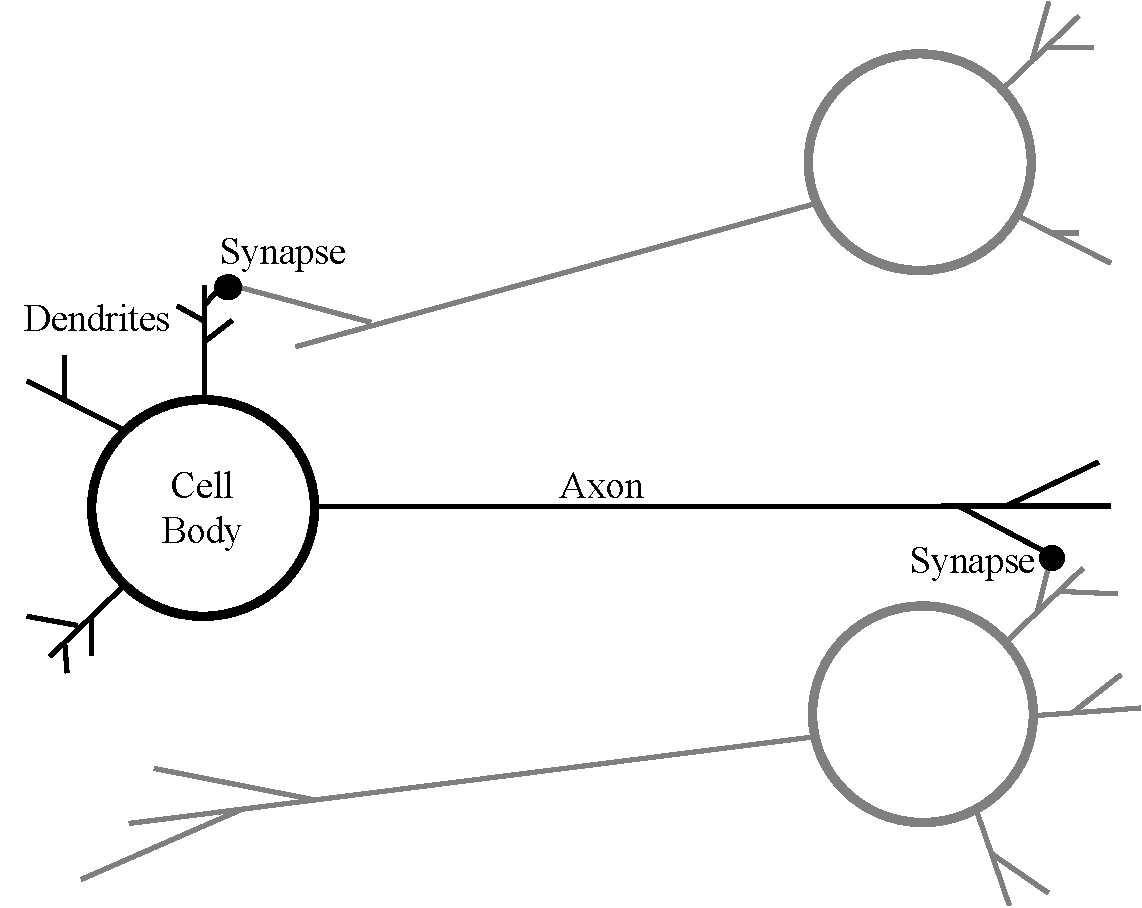
\includegraphics[width=0.6\textwidth]{./images/fmlpda_8_01.pdf}
}
\caption[A high-level schematic of the structure of a neuron.]{A high-level schematic of the structure of a neuron. This figure illustrates three interconnected neurons; the middle neuron is highlighted in black, and the major structural components of this neuron are labeled cell body, dendrites, and axon. Also marked are the synapses connecting the axon of one neuron and the dendrite of another, which allow signals to pass between the neurons. }
\label{fig:dlfig1-brainneuron}
\end{figure}
\end{frame} 


\SectionSlide{Fundamentals}

\subsection{Artificial Neurons}

 \begin{frame} 
	\begin{alignat}{2}
z & =  \underbrace{\mathbf{w}\left[0\right]\times \mathbf{d}\left[0\right] + \mathbf{w}\left[1\right] \times \mathbf{d}\left[1\right] + \dots + \mathbf{w}\left[m\right] \times \mathbf{d}\left[m\right]}_{weighted~sum} \\
	& =  \sum_{j=0}^{m} \mathbf{w}\left[j\right]\times \mathbf{d}\left[j\right] \notag\\
& = \underbrace{\mathbf{w} \cdot \mathbf{d}}_{dot~product} = \underbrace{\mathbf{w}^T \mathbf{d}}_{matrix~product} = [w_0,w_1,\dots,w_m] \begin{bmatrix}
       d_{0} \\
       d_{2} \\
       \vdots \\
       d_{m}
     \end{bmatrix}
\label{eqn:weightedsum}
	\end{alignat}
\end{frame} 



 \begin{frame} 
	\begin{equation}
\mathbb{M}_{\mathbf{w}}(\mathbf{d}) = 	\begin{cases}
		1 & \text{if } z \geq \theta\\
		0 & otherwise
	\end{cases}
	\label{eqn:thresholdfunction}
\end{equation}
\begin{equation}
	rectifier(z)=max(0,z)
	\label{eqn:rectifier}
\end{equation}
\end{frame} 



 \begin{frame} 
\begin{figure}[t]
\centerline{
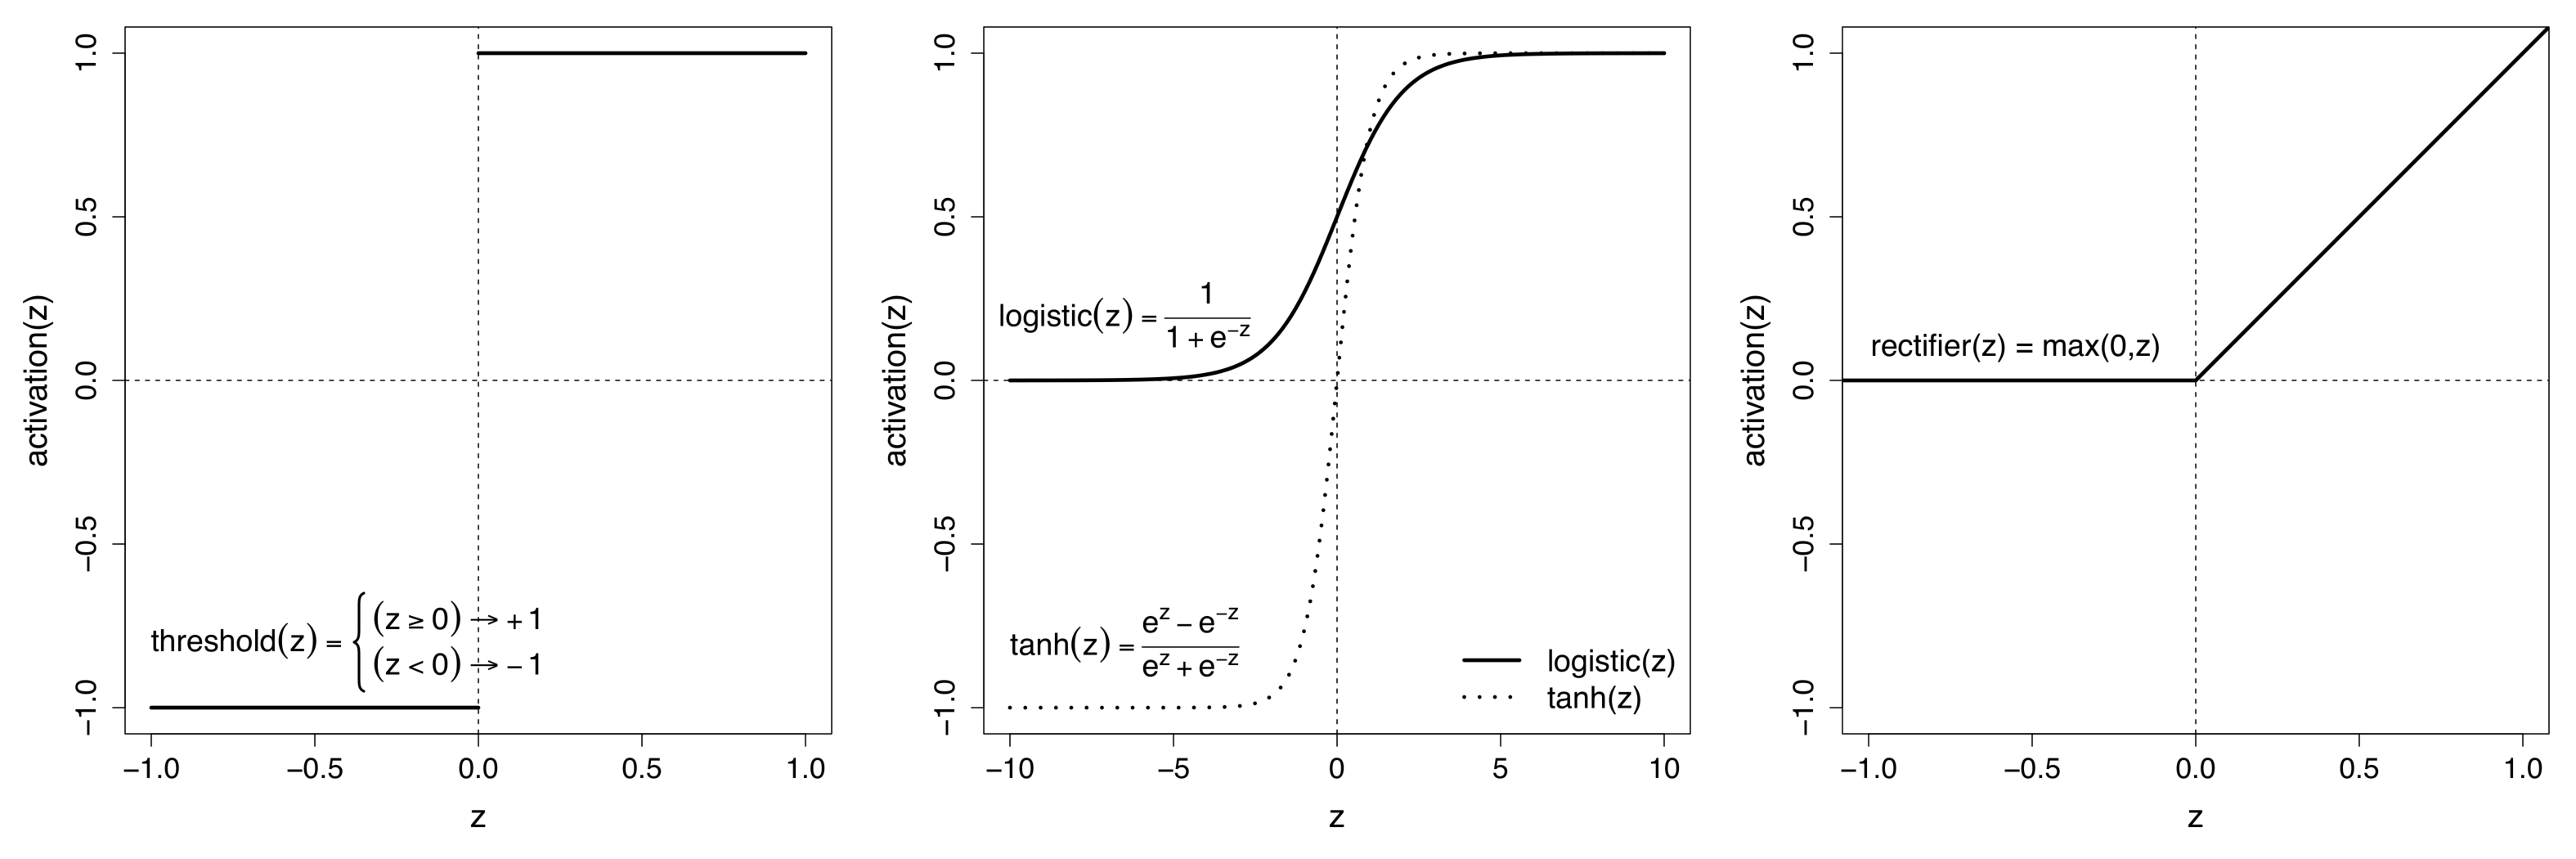
\includegraphics[width=\linewidth]{./images/fmlpda_8_02.pdf}
}
\caption[Plots for activation functions that have been popular in the history of neural networks.]{Plots for activation functions that have been popular in the history of neural networks.}
\label{fig:activationfunctions}
\end{figure}
\end{frame} 



 \begin{frame} 
\begin{alignat}{2}
	\mathbb{M}_{\mathbf{w}}(\mathbf{d}) &=  \varphi\left(\mathbf{w}\left[0\right] \times \mathbf{d}\left[0\right] + \mathbf{w}\left[1\right] \times \mathbf{d}\left[1\right] + \dots + \mathbf{w}\left[m\right] \times \mathbf{d}\left[m\right]\right) \notag \\
	 &=  \varphi \left( \sum_{i=0}^{m}w_i \times d_i \right) 
	  = \varphi\left(\underbrace{\mathbf{w} \cdot \mathbf{d}}_{dot~product}\right) \notag \\ 
	  &= \varphi\left(\underbrace{\mathbf{w}^T \mathbf{d}}_{matrix~product}\right) 
	  = \varphi \left([w_0,w_1,\dots,w_m] \begin{bmatrix}
       d_{0} \\
       d_{2} \\
       \vdots \\
       d_{m}
     \end{bmatrix}\right)
	%\notag\\
	%& =  \varphi(\mathbf{w} \cdot \mathbf{d})
	\label{eqn:neuron}
\end{alignat}
\end{frame} 



 \begin{frame} 
\begin{figure}[t]
\centerline{
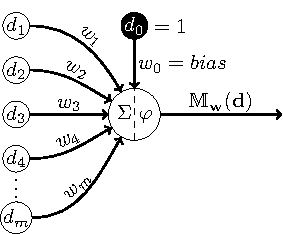
\includegraphics[width=0.5\textwidth]{./images/fmlpda_8_03.pdf}
}
\caption[A schematic of an artificial neuron.]{A schematic of an artificial neuron.}
\label{fig:artificalneuron}
\end{figure}
\end{frame} 

\subsection{Artificial Neural Networks}

 \begin{frame} 
\begin{figure}[t]
\centerline{
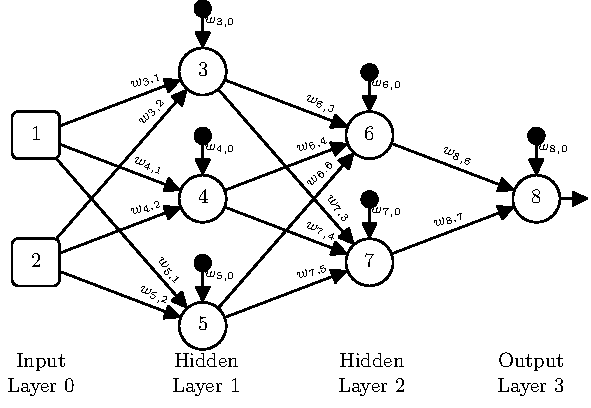
\includegraphics[width=\textwidth]{./images/fmlpda_8_04.pdf}
}
\caption[A schematic of a feedforward artificial neural network.]{A schematic of a feedforward artificial neural network.}
\label{fig:artificialneuralnetwork}
\end{figure}
\end{frame} 

\subsection{Neural Networks as Matrix Operations}


 \begin{frame} 
\begin{equation}
\mathbf{z^{(2)}=W^{(2)}a^{(1)}}
\end{equation}
\end{frame} 



 \begin{frame} 
\begin{figure}[t]
\centerline{
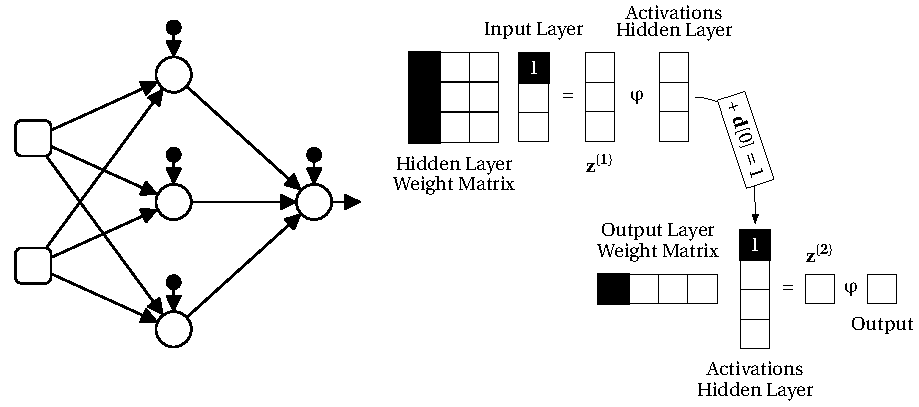
\includegraphics[width=\textwidth]{./images/fmlpda_8_05.pdf}
}
\caption[An illustration of the correspondence between graphical and matrix representations of a neural network.]{An illustration of the correspondence between graphical and matrix representations of a neural network. This figure is inspired by Figure 3.9 of \citep{kelleher:2019}.}
\label{fig:networkasmatrix}
\end{figure}
\end{frame} 



 \begin{frame} 
\begin{figure}[t]
\centerline{
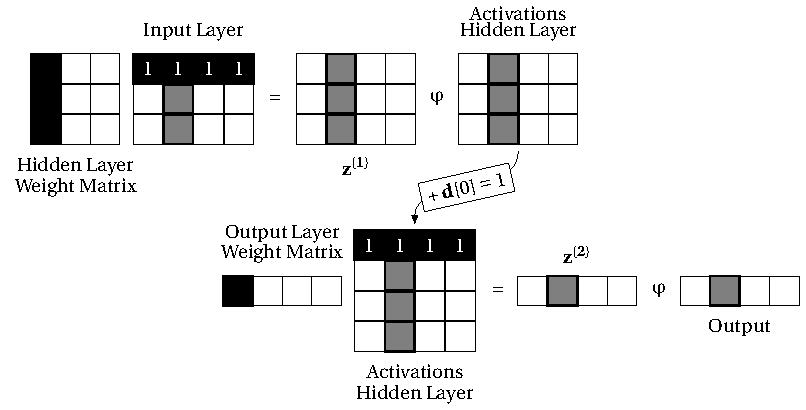
\includegraphics[width=\textwidth]{./images/fmlpda_8_06.pdf}
}
\caption[An illustration of how a batch of examples can be processed in parallel using matrix operations.]{An illustration of how a batch of examples can be processed in parallel using matrix operations.}
\label{fig:batchmatrixprocessing}
\end{figure}
\end{frame} 

\subsection{Why Are Non-Linear Activation Functions Necessary?}

 \begin{frame} 
\begin{equation}
\mathbf{A^{(1)}}=\mathbf{W^{(1)}}\mathbf{A^{(0)}}
\label{eq:firstlayer}
\end{equation}
\begin{equation}
\mathbf{A^{(2)}}=\mathbf{W^{(2)}}\mathbf{A^{(1)}}
\label{eq:secondlayer}
\end{equation}
\begin{equation}
\mathbf{A^{(2)}}=\mathbf{W^{(2)}}\left(\mathbf{W^{(1)}}\mathbf{A^{(0)}}\right)
\label{eq:rewritesecondlayer}
\end{equation}
\begin{equation}
\mathbf{A^{(2)}}=\left(\mathbf{W^{(2)}}\mathbf{W^{(1)}}\right)\mathbf{A^{(0)}}
\label{eq:associativerewrite}
\end{equation}
\begin{equation}
\mathbf{A^{(2)}}=\mathbf{W'}\mathbf{A^{(0)}}
\label{eq:associativerewrite2}
\end{equation}
\end{frame} 

\subsection{Why Is Network Depth Important?}


 \begin{frame} 
\begin{figure}[t]
\centerline{
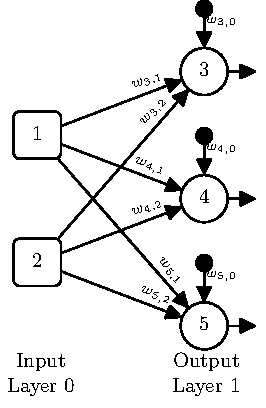
\includegraphics[width=0.4\textwidth]{./images/fmlpda_8_07.pdf}
}
\caption[A single-layer network.]{A single-layer network.}
\label{fig:perceptron}
\end{figure}
\end{frame} 



 \begin{frame} 
\begin{figure}[t]
\centerline{
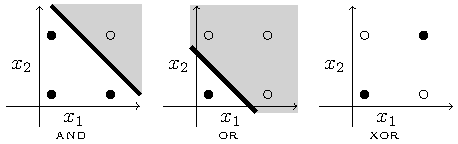
\includegraphics[width=\textwidth]{./images/fmlpda_8_08.pdf}
}
\caption[The logical \featN{AND} and \featN{OR} functions are linearly separable, but the \featN{XOR} is not.]{The logical \featN{AND} and \featN{OR} functions are linearly separable, but the \featN{XOR} is not. This figure is Figure 4.2 of \citep{kelleher:2019} and is used here with permission.}
\label{fig:linearlyseparable}
\end{figure}
\end{frame} 



 \begin{frame} 
	\begin{equation}
\mathbb{M}_{\mathbf{w}}(\mathbf{d}) = 	\begin{cases}
		1 & \text{if } z \geq 1\\
		0 & otherwise
	\end{cases}
	\label{eqn:XORNetworkThreshold}
\end{equation}
\end{frame} 

 \begin{frame} 
\begin{figure}[t]
\centerline{
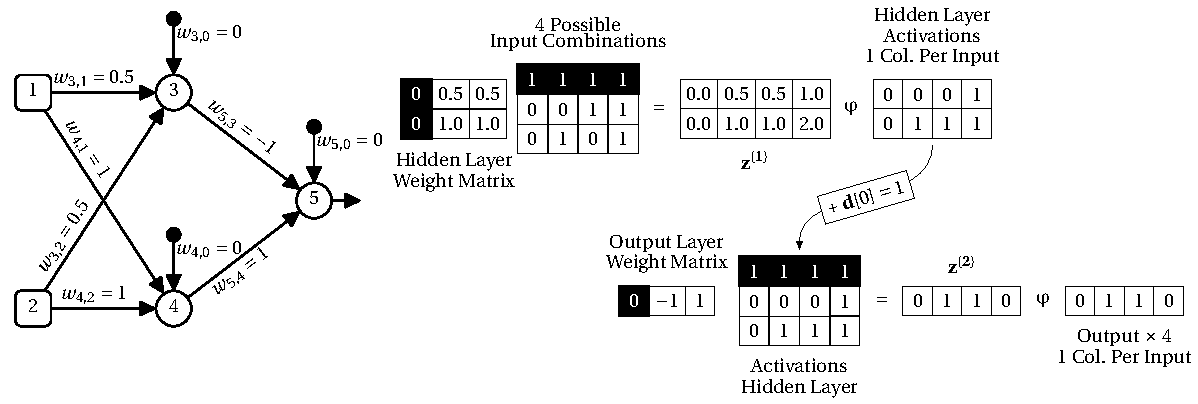
\includegraphics[width=\textwidth]{./images/fmlpda_8_09.pdf}
}
\caption[(left) The XOR function implemented as a two-layer neural network. (right) The network processing the four possible input combinations.]{(left) The XOR function implemented as a two-layer neural network. (right) The network processing the four possible input combinations, one combination plus bias input per column: [\featL{bias}, \featL{FALSE},\featL{FALSE}] $\rightarrow$  [1,0,0]; [\featL{bias}, \featL{FALSE},\featL{TRUE}] $\rightarrow$  [1,0,1]; [\featL{bias}, \featL{TRUE},\featL{FALSE}] $\rightarrow$  [1,1,0]; [\featL{bias}, \featL{TRUE},\featL{TRUE}] $\rightarrow$  [1,1,1].}
\label{fig:XORNetworkBatch}
\end{figure}
\end{frame} 



 \begin{frame} 
\begin{figure}[t]
\centerline{
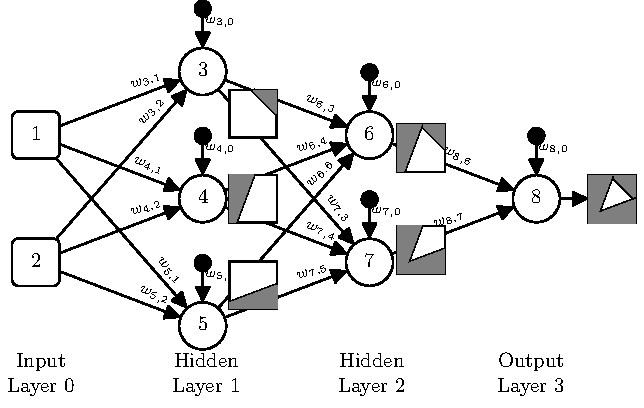
\includegraphics[width=0.9\textwidth]{./images/fmlpda_8_10.pdf}
}
\caption{An illustration of how the representational capacity of a network increases as more layers are added to the network. This figure was inspired by Figure 4.2 in \citep{ReedMarks:1999} and Figure 3.10 in \citep{marsland2011machine}.}
\label{fig:RepCapThreeLayers}
\end{figure}
\end{frame} 


\SectionSlide{Standard Approach: Backpropagation and Gradient Descent}

\subsection{Backpropagation: The General Structure of the Algorithm}

 \begin{frame} 
\begin{figure}[t]
\centerline{
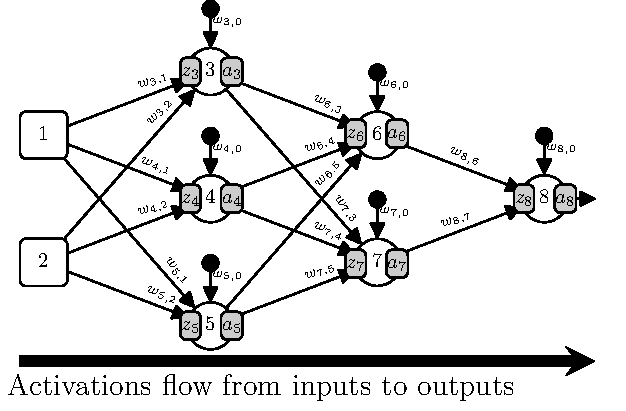
\includegraphics[width=0.9\textwidth]{./images/fmlpda_8_11.pdf}
}
\caption{The calculation of the $z$ values and activations of each neuron during the forward pass of the backpropagation algorithm. This figure is based on Figure 6.5 of \citep{kelleher:2019}.}
\label{fig:BPropForward}
\end{figure}
\end{frame} 



 \begin{frame} 
\begin{figure}[t]
\centerline{
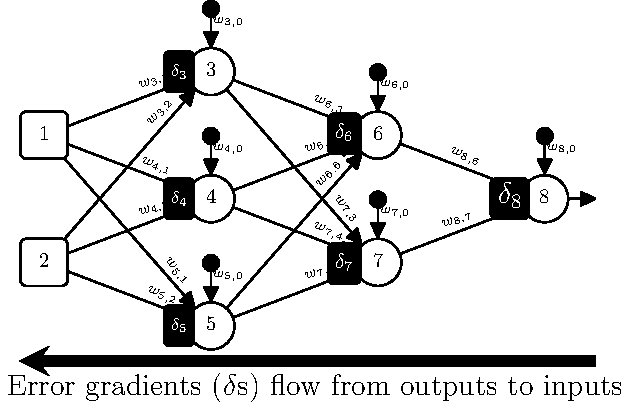
\includegraphics[width=0.9\textwidth]{./images/fmlpda_8_12.pdf}
}
\caption{The backpropagation of the $\delta$ values during the backward pass of the backpropagation algorithm. This figure is based on Figure 6.6 of \citep{kelleher:2019}.}
\label{fig:BPropBackward}
\end{figure}
\end{frame} 


\subsection{Backpropagation: Backpropagating the Error Gradients}

 \begin{frame} 
\begin{equation}
\boldsymbol{\delta}_k= \frac{\partial \mathcal{E}}{\partial z_k}
\label{eq:deltadefintion}
\end{equation}
\begin{eqnarray}
\boldsymbol{\delta}_k =  \frac{\partial a_k}{\partial z_k} \times \frac{\partial \mathcal{E}}{\partial a_k} 
\label{eq:deltaproduct}
\end{eqnarray}
\end{frame} 


 \begin{frame} 
\begin{eqnarray}
	\frac{d}{dz} logistic(z) =  logistic(z) \times (1 - logistic(z)) 
	\label{eqn:derivativeLogisticNNexample}
\end{eqnarray}
\begin{alignat}{2}
	\frac{d}{dz} logistic(z=0) & =  logistic(0) \times (1 - logistic(0)) \notag\\
	 & =  0.5 \times (1 - 0.5) \notag\\
	 & =  0.25 \notag\\
	\label{eqn:derivativeLogisticExam}
\end{alignat}
\end{frame} 



 \begin{frame} 
\begin{figure}[t]
\centerline{
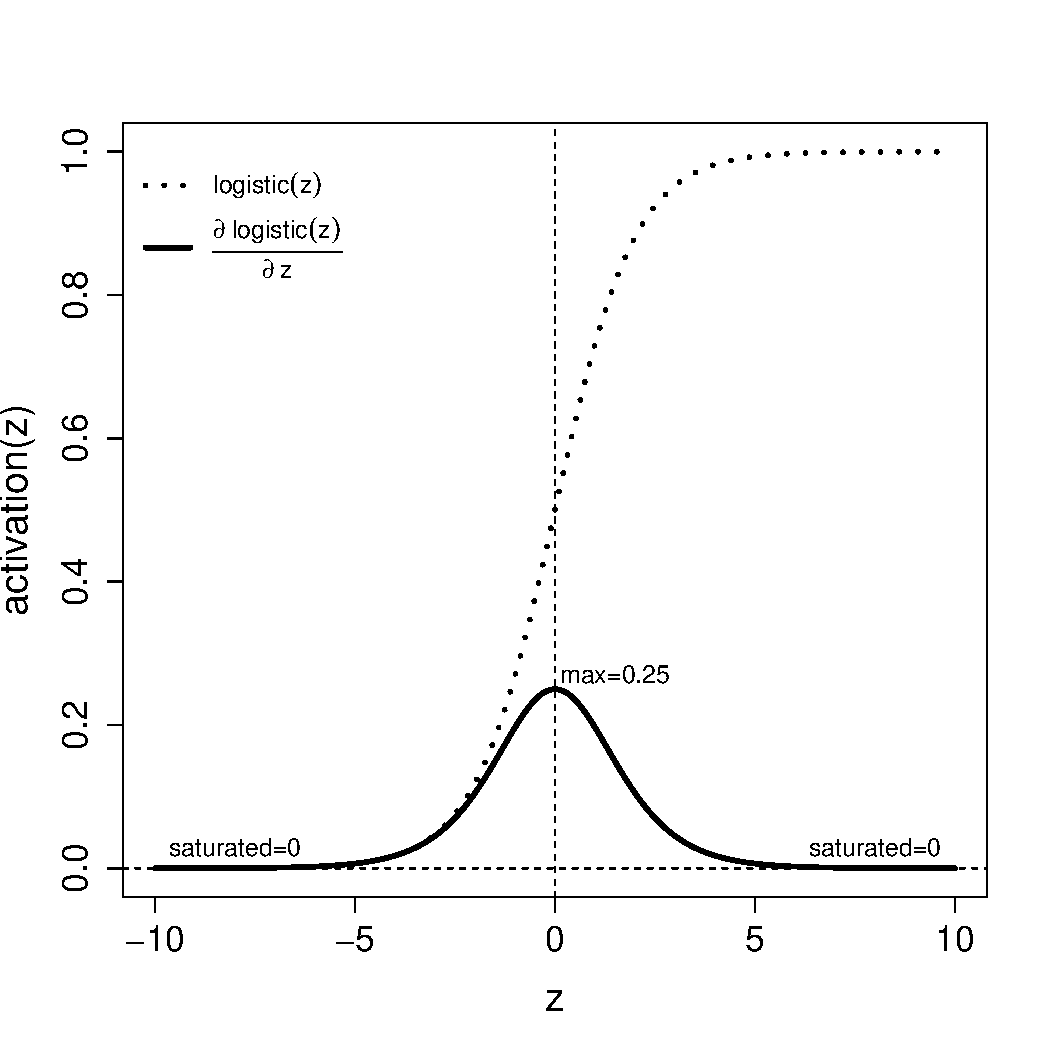
\includegraphics[width=0.6\textwidth]{./images/fmlpda_8_13.pdf}
}
\caption[Plots of the logistic function and its derivative.]{Plots of the logistic function and its derivative. This figure is Figure 4.6 of \citep{kelleher:2019} and is used here with permission.}
\label{fig:logisticderivative}
\end{figure}
\end{frame} 



 \begin{frame} 
\begin{alignat}{2}
L_2(\mathbb{M}_{\mathbf{w}}, \mathcal{D}) & = \frac{1}{2} \sum_{i=1}^{n} \left(t_i - \mathbb{M}_{\mathbf{w}}\left(\mathbf{d}_i\right)\right)^2
\label{eq:l2LossFuncNeuralNetwork}
\end{alignat}
\begin{equation}
\frac{\partial}{\partial \mathbf{w}\left[j\right]} L_2 \left( \mathbb{M}_{\mathbf{w}}, \mathbf{d} \right) =  (t - \mathbb{M}_{\mathbf{w}}(\mathbf{d})) \times -\mathbf{d}\left[j\right] \label{eqn:l2linearregressionderivative} 
\end{equation}
\begin{equation}
\frac{\partial \mathcal{E}}{\partial a_k} = \frac{\partial L_2 \left( \mathbb{M}_{\mathbf{w}}, \mathbf{d} \right)}{\partial \mathbb{M}_{\mathbf{w}}(\mathbf{d}))} =  t - \mathbb{M}_{\mathbf{w}}(\mathbf{d}) = t_k - a_k
\end{equation}
\begin{equation}
\frac{\partial \mathcal{E}}{\partial a_k} = - \left(t_k - a_k\right)
\label{eq:outputneuronerroderivative}
\end{equation}
\end{frame} 



 \begin{frame} 
\begin{alignat}{5}
\boldsymbol{\delta}_k & = & \omit\hfill $\displaystyle \frac{\partial a_k}{\partial z_k}$\hfill & \times & \omit\hfill $\displaystyle \frac{\partial \mathcal{E}}{\partial a_k}$\hfill \notag \\
& = & \omit\hfill $\displaystyle \frac{\partial a_k}{\partial z_k}$\hfill & \times & {-}\left(t_k - a_k\right)  \notag \\
& = & \omit\hfill $\underbrace{\frac{d}{dz} logistic(z)}_{\text{Assuming a logistic activation function}}$\hfill & \times &  {-}\left(t_k - a_k\right) \notag \\
& = & \underbrace{\left( logistic(z) \times (1 - logistic(z)) \right)}_{\text{Assuming a logistic activation function}} & \times & {-}\left(t_k - a_k\right) 
\label{eq:deltaforoutput}
\end{alignat}
\end{frame} 



 \begin{frame} 
\begin{equation*}
\circled{k}\!\!\rightarrow\!\!\circled{i}
\end{equation*}
\begin{equation}
\frac{\partial \mathcal{E}}{\partial a_k}=\sum^n_{i=1} w_{i,k} \times \boldsymbol{\delta}_i
	\label{eqn:propagatingHiddenDeltas}
\end{equation}
\begin{alignat}{5}
\boldsymbol{\delta}_k & = & \omit\hfill $\displaystyle \frac{\partial a_k}{\partial z_k}$\hfill & \times & \omit\hfill $\displaystyle \frac{\partial \mathcal{E}}{\partial a_k}$\hfill \notag \\
& = & \omit\hfill $\displaystyle \frac{\partial a_k}{\partial z_k}$\hfill & \times & \left(\sum^n_{i=1} w_{i,k} \times \boldsymbol{\delta}_i \right)\notag \\
& = & \omit\hfill $\underbrace{\frac{d}{dz} logistic(z)}_{\text{Assuming a logistic activation function}}$\hfill & \times &  \left(\sum^n_{i=1} w_{i,k} \times \boldsymbol{\delta}_i \right)\notag \\
& = & \underbrace{\left( logistic(z) \times (1 - logistic(z)) \right)}_{\text{Assuming a logistic activation function}} & \times & \left(\sum^n_{i=1} w_{i,k} \times \boldsymbol{\delta}_i\right) 
\label{eq:deltaforhidden}
\end{alignat}
\end{frame} 

\subsection{Backpropagation: Updating the Weights in a Network}

 \begin{frame} 
\begin{alignat}{2}
\frac{\partial \mathcal{E}}{\partial w_{i,k}} &= \frac{\partial \mathcal{E}}{\partial a_i} \times  \frac{\partial a_i}{\partial z_i} &\times \frac{\partial z_i}{\partial w_{i,k}}
\label{eq:chainerrorweight}
\end{alignat}
\begin{alignat}{5}
\frac{\partial \mathcal{E}}{\partial w_{i,k}} &= \frac{\partial \mathcal{E}}{\partial a_i} &\times&  \frac{\partial a_i}{\partial z_i} & \times &\frac{\partial z_i}{\partial w_{i,k}} \notag\\
&= &\boldsymbol{\delta}_i& & \times  &\frac{\partial z_i}{\partial w_{i,k}} \notag\\
\label{eq:chainsimplified}
\end{alignat}
\begin{equation}
\frac{\partial z_i}{\partial w_{i,k}} = a_k
\label{eq:zderivative}
\end{equation}
\end{frame} 



 \begin{frame} 
\begin{alignat}{5}
\frac{\partial \mathcal{E}}{\partial w_{i,k}} &= \frac{\partial \mathcal{E}}{\partial a_i} &\times&  \frac{\partial a_i}{\partial z_i} & \times &\frac{\partial z_i}{\partial w_{i,k}} \notag\\
&= &\boldsymbol{\delta}_i& & \times  &\frac{\partial z_i}{\partial w_{i,k}} \notag\\
&= &\boldsymbol{\delta}_i& & \times   &~~~a_k
\label{eq:chainfullysimplified}
\end{alignat}
\end{frame} 



 \begin{frame} 
\begin{equation}
w_{i,k}  \leftarrow w_{i,k} - \alpha \times \boldsymbol{\delta}_i \times  a_k
\label{eq:weightupdaterule}
\end{equation}
\end{frame} 



 \begin{frame} 
\begin{alignat}{2}
\Delta w_{i,k} &= \sum_{j=1}^m \boldsymbol{\delta}_{i,j} \times  a_{k,j} \label{eq:epochweightgradient}\\
w_{i,k} &\leftarrow w_{i,k} - \alpha \times \Delta w_{i,k}
\label{eqn:batchweightupdaterule}
\end{alignat}
\end{frame} 


\subsection{Backpropagation: The Algorithm}

\begin{frame}
%\begin{algorithm}[!t]
%\caption[The backpropagation algorithm for a feedforward network with L layers]{The backpropagation algorithm for a feedforward network with L layers}
%\label{alg:backprop}
\scriptsize
\begin{algorithmic}[1]
\Require set of training instances $\mathcal{D}$
\Require a learning rate $\alpha$ that controls how quickly the algorithm converges
\Require a batch size $B$ specifying the number of examples in each batch
\Require a convergence criterion 
\end{algorithmic}
%\end{algorithm}
\end{frame}


\begin{frame}[plain]
%\begin{algorithm}[H]
\tiny
%\fontsize{5}{6}
%\caption{\tiny Backpropagation for a feedforward net with L layers}
%\label{alg:backprop}
\begin{algorithmic}[1]
%\Require set of training instances $\mathcal{D}$
%\Require a learning rate $\alpha$ that controls how quickly the algorithm converges
%\Require a batch size $B$ specifying the number of examples in each batch
%\Require a convergence criterion 

\State Shuffle $\mathcal{D}$ and create the mini-batches: $[(\mathbf{X}^{(1)},\mathbf{Y}^{(1)}), \dots, (\mathbf{X}^{k},\mathbf{Y}^{k})]$ \label{algLine:minibatchinit}
\State Initialize the weight matrices for each layer: $\mathbf{W}^{(1)}, \dots, \mathbf{W}^{(L)}$ \label{algLine:weightinit}

\Repeat \label{algLine:epochloop}
\Comment{Each repeat loop is one epoch}
\For{t=1 to number of mini-batches} \label{algLine:forloop}
	\Comment{Each for loop is one iteration}
	\State $\mathbf{A}^{(0)}\leftarrow \mathbf{X}^{(t)}$ \label{algLine:inputs}
	
%	\Comment{Forward propagation}
	\For{$l$=1 to L} \label{algLine:forwardstart}
		\State $\mathbf{v} \leftarrow [1_0, \dots 1_m]$ \label{algLine:biasvector}
		\Comment{Create $\mathbf{v}$ the vector of bias terms}
		\State $\mathbf{A}^{(l-1)} \leftarrow [\mathbf{v};\mathbf{A}^{(l-1)}]$ \label{algLine:biasinsertion}
		\Comment{Insert $\mathbf{v}$ into the activation matrix}
		\State $\mathbf{Z}^{(l)} \leftarrow \mathbf{W}^{l} \mathbf{A}^{(l-1)}$ \label{algLine:weightsbyactivations}
		\State $\mathbf{A}^{(l)} \leftarrow \varphi(\mathbf{Z}^{(l)})$ \label{algLine:activationFunctions}
		\Comment{Elementwise application of $\varphi$ to $\mathbf{Z}^{(l)}$}
	\EndFor \label{algLine:forwardend}

	\For{each weight $w_{i,k}$ in the network} \label{algLine:startSumInit}
		\State $\Delta w_{i,k} = 0$
	\EndFor \label{algLine:endSumInit}
	
	\For{each example in the mini-batch} \label{algLine:backpropbatch}
			\Comment{Backpropagate the $\delta$s}
		\For{each neuron $i$ in the output layer}	\label{algLine:deltasoutput}
			\State $\delta_i = \frac{\partial \mathcal{E}}{\partial{a_i}} \times \frac{\partial a_i}{\partial z_i}$ \label{algLine:deltaCalc1}
			\Comment See Equation \ourEqRef{eq:deltaforoutput} 
		\EndFor \label{algLine:deltasoutputend}
		\For{$l$ = L-1 to 1} \label{algLine:deltahidden}
			\For{each neuron $i$ in the layer $l$}	
				\State $\delta_i = \frac{\partial \mathcal{E}}{\partial{a_i}} \times \frac{\partial a_i}{\partial z_i}$ \label{algLine:deltaCalc2}
				\Comment See Equation \ourEqRef{eq:deltaforhidden}
			\EndFor 
		\EndFor \label{algLine:deltahiddenend}
		
%		\Comment For each weight $w_{i,k}$ accumulate $\Delta w_{i,k}$ across the mini-batch% as we iterate through the the mini-batch 
		\For{each weight $w_{i,k}$ in the network} \label{algLine:weightsum}
			\State $\Delta w_{i,k} = \Delta w_{i,k} + (\delta_i \times a_k)$
			\Comment Equation \ourEqRef{eq:epochweightgradient}
		\EndFor \label{algLine:weightsumend}
	\EndFor \label{algLine:backpropbatchend}
	
%	\Comment Update the weights 
	\For{each weight $w_{i,k}$ in the network} \label{algLine:weightupdate}
		\State $w_{i,k} \leftarrow w_{i,k} - \alpha \times \Delta w_{i,k}$ 
		\Comment Equation \ourEqRef{eqn:batchweightupdaterule}
	\EndFor \label{algLine:weightupdateend}
\EndFor \label{algLine:minibatchend}
\State shuffle($[(\mathbf{X}^{(1)},\mathbf{Y}^{(1)}), \dots, (\mathbf{X}^{k},\mathbf{Y}^{k})]$) \label{algLine:shuffle}

\Until{convergence occurs} \label{algLine:epochloopend}
\end{algorithmic}
%\end{algorithm}
\end{frame}

\subsection{A Worked Example: Using Backpropagation to Train a Feedforward Network for a Regression Task}

 \begin{frame} 
\begin{table}
\caption[Hourly samples of ambient factors and full load electrical power output of a combined cycle power plant.] {Hourly samples of ambient factors and full load electrical power output of a combined cycle power plant.}
\label{tab:rawpowerplandata}
\noindent\resizebox{\textwidth}{!}{
\begin{tabular}{cccc}
\hline
\featN{ID} & \featN{Ambient Temperature} & \featN{Relative Humidity} & \featN{Electrical Output}\\
~ & $^\circ$C & \% & MW\\
\hline
1 & 03.21	& 86.34 & 491.35\\
2 & 31.41 & 68.50 &	430.37\\
3 &19.31 & 30.59 & 463.00\\
4 & 20.64 & 99.97 & 447.14\\
\hline
\end{tabular}
}
\end{table}
\end{frame} 



 \begin{frame} 
\begin{table}
\caption {The minimum and maximum values for the \featN{Ambient Temperature}, \featN{Relative Humidity}, and \featN{Electrical Output} features in the power plant dataset.}
\label{tab:powerplantminmax}
\noindent\resizebox{\textwidth}{!}{
\begin{tabular}{cccc}
\hline
~ & \featN{Ambient Temperature} & \featN{Relative Humidity} & \featN{Electrical Output}\\
\hline
Min & $1.81^\circ$C & 25.56\% & 420.26MW\\
Max & $37.11^\circ$C & 100.16\% &	495.76MW\\
\hline
\end{tabular}
}
\end{table}
\end{frame} 



 \begin{frame} 
\begin{table}
\caption {The \emph{range-normalized} hourly samples of ambient factors and full load electrical power output of a combined cycle power plant, rounded to two decimal places.}
\label{tab:normalizedpowerplandata}
\noindent\resizebox{\textwidth}{!}{
\begin{tabular}{cccc}
\hline
\featN{ID} & \featN{Ambient Temperature} & \featN{Relative Humidity} & \featN{Electrical Output}\\
~ & $^\circ$C & \% & MW\\
\hline
1 & 0.04 & 0.81 & 0.94\\
2 & 0.84 & 0.58 & 0.13\\
3 & 0.50 & 0.07 & 0.57\\
4 & 0.53 & 1.00 & 0.36\\
\hline
\end{tabular}
}
\end{table}
\end{frame} 



 \begin{frame} 
\begin{figure}
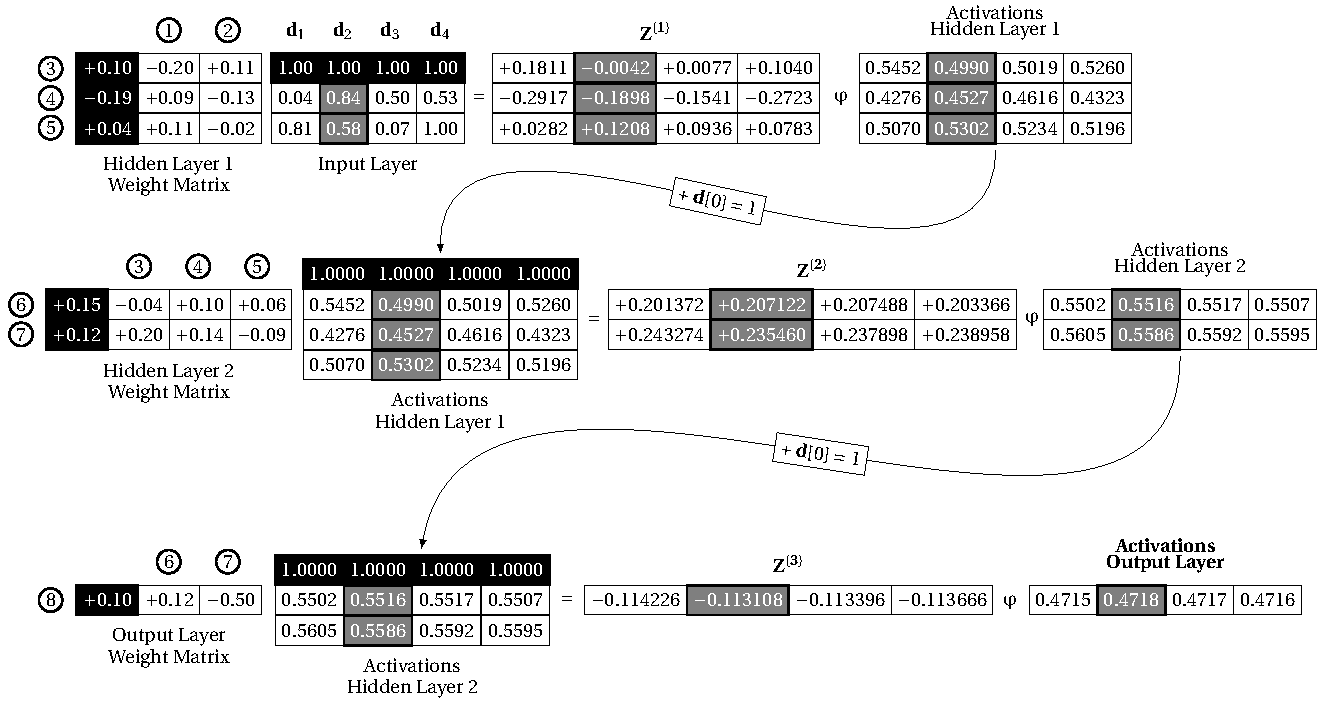
\includegraphics[width=\textwidth]{./images/fmlpda_8_14.pdf}
\caption{The forward pass of the examples listed in Table \ourRef{tab:normalizedpowerplandata} through the network in Figure \ourRef{fig:artificialneuralnetwork}.}
\label{fig:forwardpass}
\end{figure}
\end{frame} 



 \begin{frame} 
\begin{table}[htb]
\caption {The per example error after the forward pass illustrated in Figure \ourRef{fig:forwardpass}, the per example $\partial \mathcal{E}/\partial {a_8}$, and the \keyword{sum of squared errors} for the model over the dataset of four examples.}
\label{tab:nnexampleerrors}
\noindent\resizebox{\textwidth}{!}{
\begin{tabular}{lrrrr}
\hline
~ & $\mathbf{d}_1$ & $\mathbf{d}_2$ & $\mathbf{d}_3$ & $\mathbf{d}_4$\\
\hline
Target & 0.9400 & 0.1300 & 0.5700 & 0.3600\\
Prediction & 0.4715 & 0.4718 & 0.4717 & 0.4716\\
Error & 0.4685 & {-0.3418} & 0.0983 & {-0.1116}\\
$\partial \mathcal{E}/\partial {a_8}$: Error $\times {-1}$& {-0.4685} & 0.3418 & {-0.0983} & 0.1116\\
\hline
Error$^2$ & 0.21949225 & 0.11682724 & 0.00966289 &0.01245456 \\
SSE: & & & & 0.17921847\\%0.35843694\\
\hline
\end{tabular}
}
\end{table}
\end{frame} 



 \begin{frame} 
\begin{figure}[t]
\centerline{
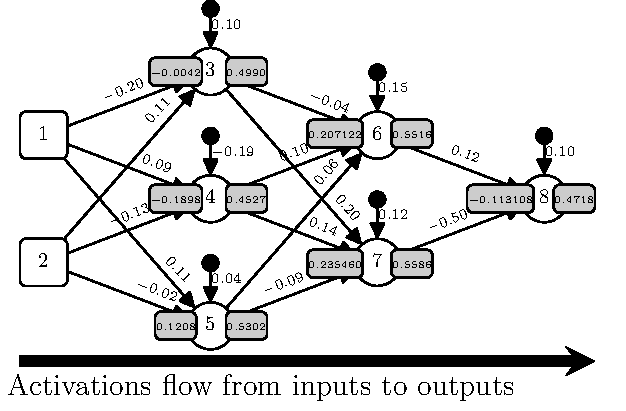
\includegraphics[width=0.9\textwidth]{./images/fmlpda_8_15.pdf}
}
\caption{An illustration of the forward propagation of $\mathbf{d}_2$ through the network showing the weights on each connection, and the weighted sum $z$ and activation $a$ value for each neuron in the network.}
\label{fig:forwardpassExample2}
\end{figure}
\end{frame} 



 \begin{frame} 
\begin{equation}
\frac{\partial \mathcal{E}}{\partial a}=0.3418
\end{equation}
\begin{alignat}{3}
\delta_8 & = & \frac{\partial \mathcal{E}}{\partial a_8} &\times \frac{\partial a_8}{\partial z_8} \notag\\
& = & 0.3418 &\times 0.2492 \notag\\
& = & 0.0852
\label{eq:delta8calc}
\end{alignat}
\end{frame} 



 \begin{frame} 
\begin{table}[htb]
\caption {The $\partial a/\partial z$ for each neuron for Example 2 rounded to four decimal places.}
\label{tab:activationfunctionderivatives}
\begin{tabular}{crc}
\hline
\featN{Neuron} & $z$ & $\partial a/\partial z$\\
\hline
3 & -0.004200& 0.2500\\
4 & -0.189800& 0.2478\\
5 & 0.120800& 0.2491\\
6 & 0.207122& 0.2473\\
7 & 0.235460& 0.2466\\
8 & -0.113108& 0.2492\\
\hline
\end{tabular}
\end{table}
\end{frame} 



 \begin{frame} 
\begin{alignat}{3}
\delta_6 & = & \frac{\partial \mathcal{E}}{\partial a_6} &\times \frac{\partial a_6}{\partial z_6} \notag\\
& = & \left(\sum \delta_i \times w_{i,6}\right) &\times \frac{\partial a_6}{\partial z_6} \notag\\
& = & \left(\delta_8 \times w_{8,6}\right) &\times \frac{\partial a_6}{\partial z_6} \notag\\
& = & \left(0.0852 \times 0.12\right) &\times 0.2473\notag\\
& = & 0.0025
\label{eq:delta6}
\end{alignat}
\end{frame} 



 \begin{frame} 
\begin{alignat}{3}
\delta_7 & = & \frac{\partial \mathcal{E}}{\partial a_7} &\times \frac{\partial a_7}{\partial z_7} \notag\\
& = & \left(\sum \delta_i \times w_{i,7}\right) &\times \frac{\partial a_7}{\partial z_7} \notag\\
& = & \left(\delta_8 \times w_{8,7}\right) &\times \frac{\partial a_6}{\partial z_6} \notag\\
& = & \left(0.0852 \times {-0.50}\right) &\times 0.2466 \notag\\
& = & {-0.0105}
\label{eq:delta7}
\end{alignat}
\end{frame} 



 \begin{frame} 
\begin{alignat}{3}
\delta_3 & = & \frac{\partial \mathcal{E}}{\partial a_3} &\times \frac{\partial a_3}{\partial z_3} \notag\\
& = & \left(\sum \delta_i \times w_{i,3}\right) &\times \frac{\partial a_3}{\partial z_3} \notag\\
& = & \left(\left(\delta_6 \times w_{6,3}\right) + \left(\delta_7 \times w_{7,3}\right) \right) &\times \frac{\partial a_3}{\partial z_3} \notag\\
& = & \left(\left(0.0025 \times -0.04\right) + \left({-0.0105} \times 0.20\right) \right) &\times 0.2500\notag\\
& = & {-0.0006}
\label{eq:delta3}
\end{alignat}
\end{frame} 



 \begin{frame} 
\begin{alignat}{3}
\delta_4 & = & \frac{\partial \mathcal{E}}{\partial a_4} &\times \frac{\partial a_4}{\partial z_4} \notag\\
& = & \left(\sum \delta_i \times w_{i,4}\right) &\times \frac{\partial a_4}{\partial z_4} \notag\\
& = & \left(\left(\delta_6 \times w_{6,4}\right) + \left(\delta_7 \times w_{7,4}\right) \right) &\times \frac{\partial a_4}{\partial z_4} \notag\\
& = & \left(\left(0.0025 \times 0.10\right) + \left({-0.0105} \times 0.14\right) \right) &\times 0.2478\notag\\
& = & {-0.0003}
\label{eq:delta4}
\end{alignat}
\end{frame} 



 \begin{frame} 
\begin{alignat}{3}
\delta_5 & = & \frac{\partial \mathcal{E}}{\partial a_5} &\times \frac{\partial a_5}{\partial z_5} \notag\\
& = & \left(\sum \delta_i \times w_{i,5}\right) &\times \frac{\partial a_5}{\partial z_5} \notag\\
& = & \left(\left(\delta_6 \times w_{6,5}\right) + \left(\delta_7 \times w_{7,5}\right) \right) &\times \frac{\partial a_5}{\partial z_5} \notag\\
& = & \left(\left(0.0025 \times 0.06\right) + \left({-0.0105} \times -0.09\right) \right) &\times 0.2491\notag\\
& = & 0.0003
\label{eq:delta5}
\end{alignat}
\end{frame} 



 \begin{frame} 
\begin{figure}[t]
\centerline{
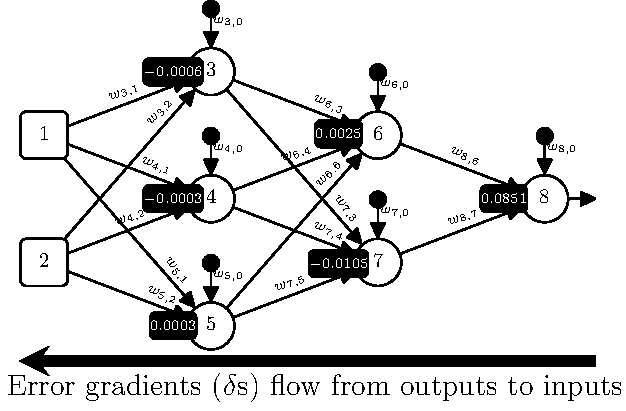
\includegraphics[width=0.9\textwidth]{./images/fmlpda_8_16.pdf}
}
\caption{The $\delta$s for each of the neurons in the network for Ex. 2.} 
\label{fig:networkdeltasEx2}
\end{figure}
\end{frame} 



 \begin{frame}[plain] 
\begin{table}[!tb]
\caption {The $\partial \mathcal{E}/\partial w_{i,k}$ calculations for $\mathbf{d}_2$ for every weight in the network. The neuron index 0 denotes the bias input for each neuron.}
\label{tab:networkweightsensitivities}
\vspace{-0.75cm}
\noindent\resizebox{\textwidth}{!}{
%\begin{tabular*}{\linewidth}{@{\extracolsep{\fill}} cccrrr @{}}
\begin{tabular}{cccrrr}
\hline
\featN{Neuron}$_i$ & \featN{Neuron}$_k$ & $w_{i,k}$ & $\delta_i$ & $a_k$ & $\partial \mathcal{E}/\partial w_{i,k}$\\
\hline
8 & 0 & $w_{8,0}$ & $0.0852$ & $1$ & $0.0852 \times 1 = 0.0852$\\
8 & 6 & $w_{8,6}$ & $0.0852$ & $0.5516$ & $ 0.0852 \times 0.5516 = 0.04699632$\\
8 & 7 & $w_{8,7}$ & $0.0852$ & $0.5586$ & $ 0.0852 \times 0.5586 = 0.04759272$\\
7 & 0 & $w_{7,0}$ & ${-0.0105}$ & $1$ & ${-0.0105} \times 1 = {-0.0105}$\\
7 & 3 & $w_{7,3}$ & ${-0.0105}$ & $0.4990$ & ${-0.0105} \times 0.4527 = {-0.0052395}$\\
7 & 4 & $w_{7,4}$ & ${-0.0105}$ & $0.4527$ & ${-0.0105} \times 0.4527 = {-0.00475335}$\\
7 & 5 & $w_{7,5}$ & ${-0.0105}$ & $0.5302$ & ${-0.0105} \times 0.5302 = {-0.0055671}$\\
6 & 0 & $w_{6,0}$ & $0.0025$ & $1$ & $0.0025 \times 1 = 0.0025$\\
6 & 3 & $w_{6,3}$ & $0.0025$ & $0.4990$ & $0.0025 \times 0.4527 = 0.0012475$\\
6 & 4 & $w_{6,4}$ & $0.0025$ & $0.4527$ & $0.0025 \times 0.4527 = 0.00113175$\\
6 & 5 & $w_{6,5}$ & $0.0025$ & $0.5302$ & $0.0025 \times 0.5302 = 0.0013255$\\
5 & 0 & $w_{5,0}$ & $0.0003$ & $1$ & $0.0003 \times 1 = 0.0003$\\
5 & 1 & $w_{5,1}$ & $0.0003$ & $0.84$ & $0.0003 \times 0.84 = 0.000252$\\
5 & 2 & $w_{5,2}$ & $0.0003$ & $0.58$ & $0.0003 \times 0.58 = 0.000174$\\
4 & 0 & $w_{4,0}$ & ${-0.0003}$ & $1$ & ${-0.0003} \times 1 = {-0.0003}$\\
4 & 1 & $w_{4,1}$ & ${-0.0003}$ & $0.84$ & ${-0.0003} \times 0.84 = {-0.000252}$\\
4 & 2 & $w_{4,2}$ & ${-0.0003}$ & $0.58$ & ${-0.0003} \times 0.58 = {-0.000174}$\\
3 & 0 & $w_{3,0}$ & ${-0.0006}$ & $1$ & ${-0.0006} \times 1 = {-0.0006}$\\
3 & 1 & $w_{3,1}$ & ${-0.0006}$ & $0.84$ & ${-0.0006} \times 0.84 = {-0.000504}$\\
3 & 2 & $w_{3,2}$ & ${-0.0006}$ & $0.58$ & ${-0.0006} \times 0.58 = {-0.000348}$\\
\hline
\end{tabular}
%\end{tabular*}
}
\end{table}
\end{frame} 



 \begin{frame} 
\begin{alignat}{4}
w_{7,5} &= ~~~w_{7,5}  &-~~~&  ~~\alpha &~~\times~~&  ~~~\boldsymbol{\delta}_7 \times  a_5 \notag\\
               ~ &= ~~~w_{7,5}  &-~~~&  ~~\alpha &~~\times~~&  ~~~\frac{\partial \mathcal{E}}{\partial w_{i,k}} \notag\\
               ~ &= -0.09~~~    &-~~~&  0.2 &~~\times~~&  {-0.0055671} \notag\\
               ~ &= {-0.08888658} &&&&                   
\label{eqn:stochasticweightupdateexmple}
\end{alignat}
\end{frame} 



 \begin{frame} 
\begin{table}
\caption {The calculation of $\Delta w_{7,5}$ across our four examples.}
\label{tab:minibatchdelta}
\begin{tabular}{cr}
\hline
\featN{Mini-batch} & \multirow{2}{*}{$\displaystyle \frac{\partial \mathcal{E}}{\partial w_{7,5}}$}\\
\featN{Example} & \\
\hline
$\mathbf{d}_1$ & $0.00730080$\\
$\mathbf{d}_2$ & ${-0.00556710}$\\
$\mathbf{d}_3$ & $0.00157020$\\
$\mathbf{d}_4$ & ${-0.00176664}$\\
\hline
$\displaystyle \Delta w_{7,5}$= & $0.00153726$\\
\hline
\end{tabular}
\end{table}
\end{frame} 



 \begin{frame} 
\begin{alignat}{1}
w_{7,5} &= w_{7,5} - \alpha \times \Delta w_{i,k} \notag\\
~ &= -0.09 - 0.2 \times 0.00153726 \notag\\
~ &= {-0.0903074520}
\label{eqn:batchweightupdateexample}
\end{alignat}
\end{frame} 



 \begin{frame} 
\begin{table}
\caption {The per example error after each weight has been updated once, the per example $\partial \mathcal{E}/\partial {a_8}$, and the \keyword{sum of squared errors} for the model.}
\label{tab:nnexampleerrorspostweightupdate}
\noindent\resizebox{\textwidth}{!}{
\begin{tabular}{lrrrr}
\hline
~ & $\mathbf{d}_1$ & $\mathbf{d}_2$ & $\mathbf{d}_3$ & $\mathbf{d}_4$\\
\hline
Target & 0.9400 & 0.1300 & 0.5700 & 0.3600\\
Prediction & 0.4738 & 0.4741 & 0.4740 & 0.4739\\
Error & 0.4662 & {-0.3441} & 0.0960 & {-0.1139}\\
$\partial \mathcal{E}/\partial {a_8}$: Error $\times {-1}$& {-0.4662} & 0.3441 & {-0.0960} & 0.1139\\
\hline
Error$^2$ & 0.21734244 & 0.11840481 & 0.009216 & 0.01297321 \\
SSE: & & & & 0.17896823\\%0.35793646\\%
\hline
\end{tabular}
}
\end{table}
\end{frame} 



 \begin{frame} 
\begin{table}
\caption {The per example prediction, error, and the sum of squared errors after training has converged to an $SSE<0.0001$.}
\label{tab:nnexampleerrorspost7656weightupdate}
\noindent\resizebox{\textwidth}{!}{
\begin{tabular}{lrrrr}
\hline
~ & $\mathbf{d}_1$ & $\mathbf{d}_2$ & $\mathbf{d}_2$ & $\mathbf{d}_2$\\
\hline
Target & 0.9400 & 0.1300 & 0.5700 & 0.3600\\
Prediction &0.9266 & 0.1342 &0.5700 & 0.3608\\
Error & 0.0134 & {-0.0042} & 0.0000 & {-0.0008}\\
\hline
Error$^2$ & 0.00017956 & 0.00001764 & 0.00000000 & 0.00000064 \\
SSE: & & & & 0.00009892\\
\hline
\end{tabular}
}
\end{table}
\end{frame} 



 \begin{frame} 
\begin{figure}[t]
\centerline{
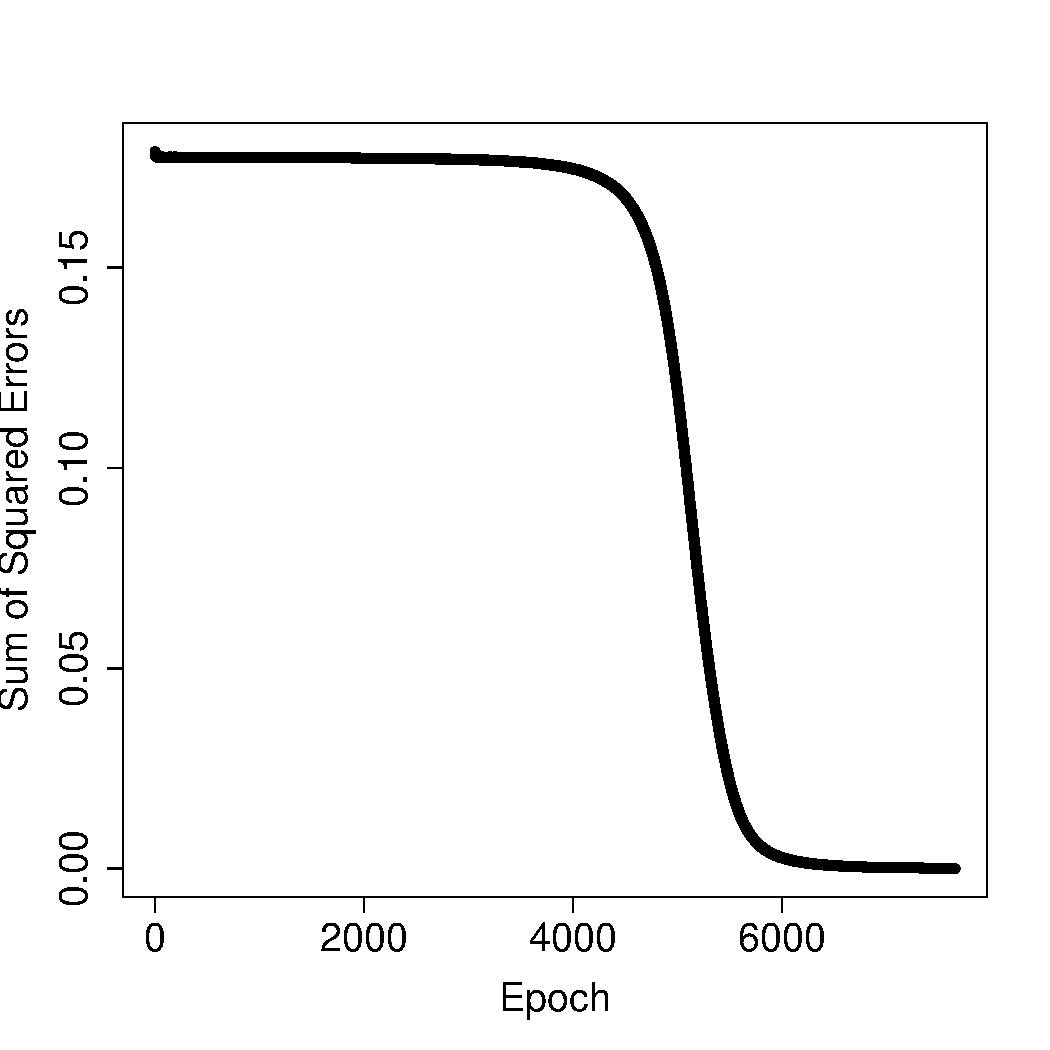
\includegraphics[width=0.5\textwidth]{./images/fmlpda_8_17.pdf}
}
\caption[A plot showing how the sum of squared errors of the network changed during training.]{A plot showing how the sum of squared errors of the network changed during training.}
\label{fig:SSEperTrainingIterationNN1}
\end{figure}
\end{frame} 


\SectionSlide{Extensions and Variations}


\subsection{Vanishing Gradients and ReLUs}

 \begin{frame} 
\begin{alignat}{5}
\frac{\partial \mathcal{E}}{\partial w_{i,k}} &= \frac{\partial \mathcal{E}}{\partial a_i} &\times&  \frac{\partial a_i}{\partial z_i} & \times &\frac{\partial z_i}{\partial w_{i,k}} \notag\\
&= &\boldsymbol{\delta}_i& & \times  &\frac{\partial z_i}{\partial w_{i,k}} \notag\\
\label{eq:vanishinggradientchainsimplified}
\end{alignat}
\end{frame} 



 \begin{frame} 
\begin{equation*}
\circled{i}\!\!\rightarrow\!\!\circled{j}\!\!\rightarrow\!\!\circled{k}
\end{equation*}
\begin{alignat}{3}
\delta_i & = & \makebox[\widthof{$w_{j,i} \times w_{k,j} \times \frac{\partial \mathcal{E}}{\partial a_k} \times \frac{\partial a_k}{\partial z_k} \times \frac{\partial a_j}{\partial z_j}\hspace{0.8em}$}]{$\displaystyle \frac{\partial \mathcal{E}}{\partial a_i}$} &\times \frac{\partial a_i}{\partial z_i} \notag\\
& = & \overbrace{w_{j,i} \times \makebox[\widthof{$w_{k,j} \times \frac{\partial \mathcal{E}}{\partial a_k} \times \frac{\partial a_k}{\partial z_k} \times \frac{\partial a_j}{\partial z_j}\hspace{0.8em}$}]{$\delta_j$}} &\times \frac{\partial a_i}{\partial z_i} \notag\\
& = & 
	w_{j,i} \times 
			\overbrace{w_{k,j} \times \makebox[\widthof{$\frac{\partial \mathcal{E}}{\partial a_k} \times \frac{\partial a_k}{\partial z_k}\hspace{0.4em}$}]{$\delta_k$} \times \frac{\partial a_j}{\partial z_j}}  
	&\times \frac{\partial a_i}{\partial z_i} \notag\\
& = & w_{j,i} \times 
			w_{k,j} \times 
				\overbrace{\frac{\partial \mathcal{E}}{\partial a_k} \times \frac{\partial a_k}{\partial z_k}}
		\times \frac{\partial a_j}{\partial z_j}  
&\times \frac{\partial a_i}{\partial z_i} \notag\\
\label{eq:chainexpansion}
\end{alignat}
\end{frame} 



 \begin{frame} 
\begin{equation}
	rectifier(z)=max(0,z)= \begin{cases}
		z & \text{if } z > 0\\
		0 & otherwise
	\end{cases}
	\label{eqn:rectifier2}
\end{equation}
\begin{equation}
\frac{d}{dz} rectifier(z) = 	\begin{cases}
		1 & \text{if } z > 0\\
		0 & otherwise
	\end{cases}
	\label{eqn:rectifierderivatve}
\end{equation}
\end{frame} 



 \begin{frame} 
\begin{figure}
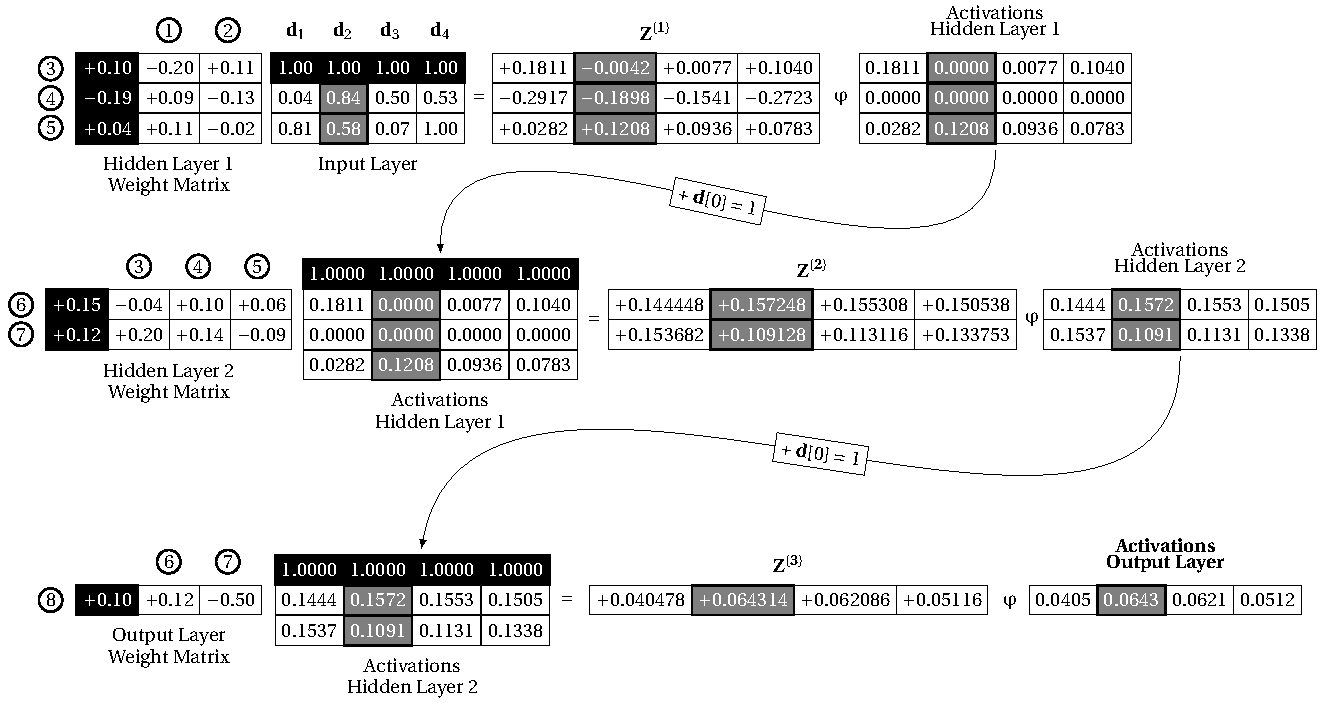
\includegraphics[width=\textwidth]{./images/fmlpda_8_18.pdf}
\caption{The forward pass of the examples listed in Table \ourRef{tab:normalizedpowerplandata} through the network in Figure \ourRef{fig:artificialneuralnetwork} when all the neurons are ReLUs.}
\label{fig:forwardpassrelus}
\end{figure}
\end{frame} 



 \begin{frame} 
\begin{figure}[!t]
\centerline{
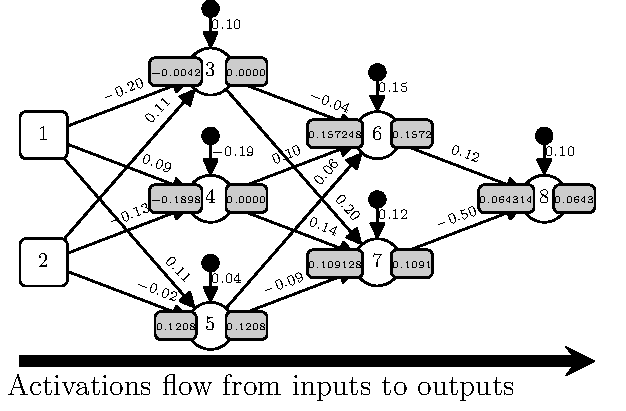
\includegraphics[width=0.9\textwidth]{./images/fmlpda_8_19.pdf}
}
\caption{An illustration of the forward propagation of $\mathbf{d}_2$ through the ReLU network showing the weights on each connection, and the weighted sum $z$ and activation $a$ value for each neuron in the network.}
\label{fig:forwardpropex2relu}
\end{figure}
\end{frame} 



 \begin{frame} 
\begin{table}[!b]
\caption {The per example error of the ReLU network after the forward pass illustrated in Figure \ourRef{fig:forwardpassrelus}, the per example $\partial \mathcal{E}/\partial {a_8}$, and the \keyword{sum of squared errors} for the ReLU model.}
\label{tab:nnReLUexampleerrors}
\noindent\resizebox{\textwidth}{!}{
\begin{tabular}{lrrrr}
\hline
~ & $\mathbf{d}_1$ & $\mathbf{d}_2$ & $\mathbf{d}_3$ & $\mathbf{d}_4$\\
\hline
Target & 0.9400 & 0.1300 & 0.5700 & 0.3600\\
Prediction & 0.0405 & 0.0643 & 0.0621 & 0.0512\\
Error & 0.8995 & 0.0657 & 0.5079 & 0.3088\\
$\partial \mathcal{E}/\partial {a_8}$: Error $\times {-1}$& ${-0.8995}$ & ${-0.0657}$ & ${-0.5079}$ & ${-0.3088}$\\
\hline
Error$^2$ & 0.80910025 & 0.00431649 & 0.25796241 & 0.09535744\\
SSE: & & & & 0.58336829\\%1.16673659\\
\hline
\end{tabular}
}
\end{table}
\end{frame} 



 \begin{frame} 
\begin{table}[htb]
\caption {The $\partial a/\partial z$ for each neuron for $\mathbf{d}_2$ rounded to four decimal places.}
\label{tab:example2ReLUderivatives}
\begin{tabular}{crc}
\hline
\featN{Neuron} & $z$ & $\partial a/\partial z$\\
\hline
3 & -0.004200& 0\\
4 & -0.189800& 0\\
5 & 0.120800& 1\\
6 & 0.157248& 1\\
7 & 0.109128& 1\\
8 & 0.064314& 1\\
\hline
\end{tabular}
\end{table}
\end{frame} 



 \begin{frame} [plain]
 \tiny
\begin{alignat}{3}
\delta_k & = & \frac{\partial \mathcal{E}}{\partial a_k} &\times \frac{\partial a_k}{\partial z_i} \notag\\
\delta_8 & = & -0.0657 &\times 1.0 \notag\\
& = & -0.0657\notag\\
\delta_7 & = & \left(\delta_8 \times w_{8,7}\right) &\times \frac{\partial a_7}{\partial z_7} \notag\\
& = & \left(-0.0657 \times {-0.50}\right) &\times 1 \notag\\
& = & {0.0329}\notag\\
\delta_6 & = & \left(\delta_8 \times w_{8,6}\right) &\times \frac{\partial a_6}{\partial z_6} \notag\\
& = & \left(-0.0657 \times 0.12\right) &\times 1\notag\\
& = & -0.0079\notag\\
\delta_5 & = & \left(\left(\delta_6 \times w_{6,5}\right) + \left(\delta_7 \times w_{7,5}\right) \right) &\times \frac{\partial a_5}{\partial z_5} \notag\\
& = & \left(\left(-0.0079 \times 0.06\right) + \left({0.0329} \times -0.09\right) \right) &\times 1\notag\\
& = & -0.0034\notag\\
\delta_4 & = & \left(\left(\delta_6 \times w_{6,4}\right) + \left(\delta_7 \times w_{7,4}\right) \right) &\times \frac{\partial a_4}{\partial z_4} \notag\\
& = & \left(\left(-0.0079 \times 0.10\right) + \left({0.0329} \times 0.14\right) \right) &\times 0\notag\\
& = & {0}\notag\\
\delta_3 & = & \left(\left(\delta_6 \times w_{6,3}\right) + \left(\delta_7 \times w_{7,3}\right) \right) &\times \frac{\partial a_3}{\partial z_3} \notag\\
& = & \left(\left(-0.0079 \times -0.04\right) + \left({0.0329} \times 0.20\right) \right) &\times 0\notag\\
& = & {0}\notag\\
\label{eq:reludeltacalc}
\end{alignat}
\end{frame} 



 \begin{frame} 
\begin{table}
\caption {The ReLU network's per example prediction, error, and the sum of squared errors after training has converged to an $SSE<0.0001$.}
\label{tab:nnReLUexampleerrorspost424weightupdate}
\noindent\resizebox{\textwidth}{!}{
\begin{tabular}{lrrrr}
\hline
~ & $\mathbf{d}_1$ & $\mathbf{d}_2$ & $\mathbf{d}_3$ & $\mathbf{d}_4$\\
\hline
Target & 0.9400 & 0.1300 & 0.5700 & 0.3600\\
Prediction &0.9487 & 0.1328 &0.5772 & 0.3679\\
Error & {-0.0087} & {-0.0028} & {-0.0072} & {-0.0079}\\
\hline
Error$^2$ & 0.00007569 &  0.00000784 & 0.00005184 & 0.00006241  \\
SSE: & & & & 0.00009889\\
\hline
\end{tabular}
}
\end{table}
\end{frame} 



 \begin{frame} 
\begin{figure}[t]
\centerline{
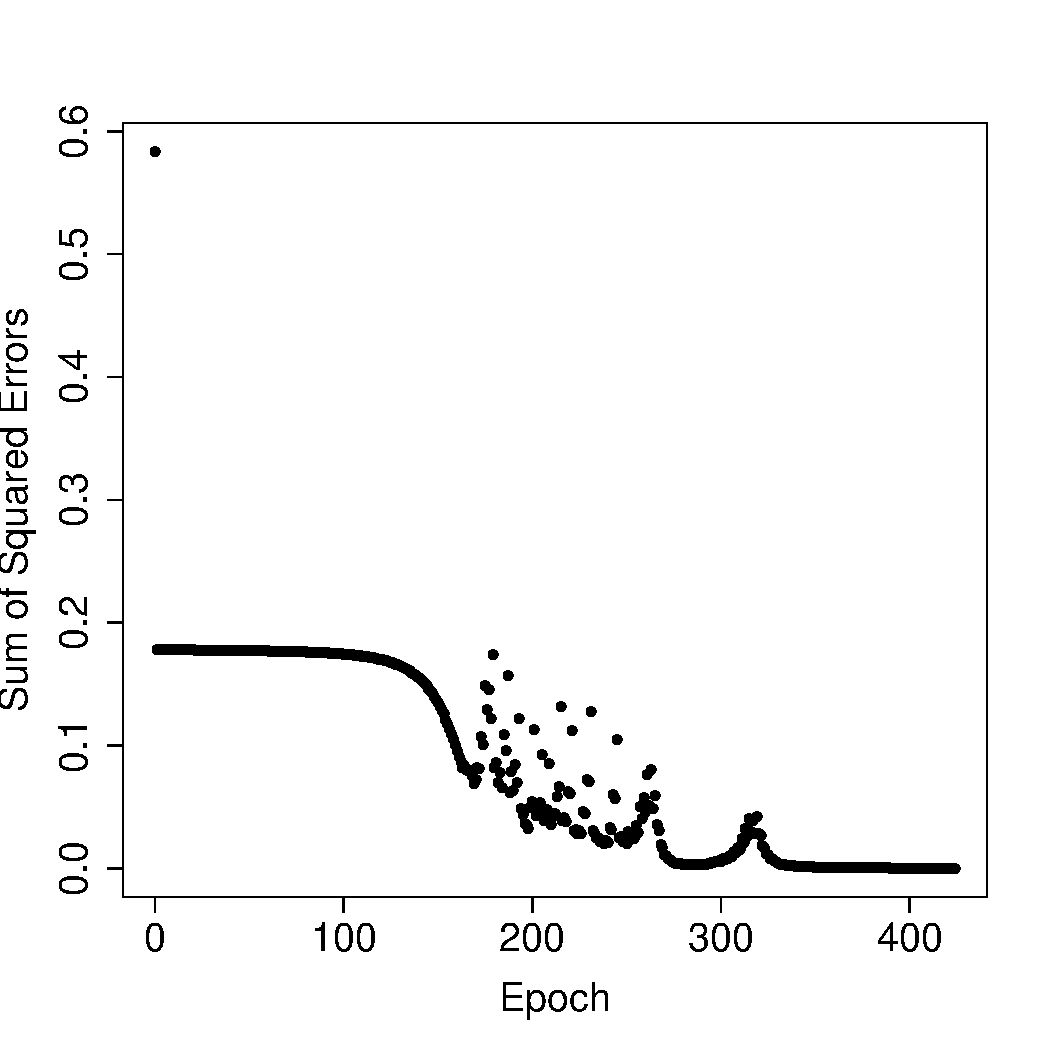
\includegraphics[width=0.5\textwidth]{./images/fmlpda_8_20.pdf}
}
\caption[A plot showing how the sum of squared errors of the ReLU network changed during training when $\alpha=0.2$.]{A plot showing how the sum of squared errors of the ReLU network changed during training when $\alpha=0.2$.}
\label{fig:SSEperTrainingIterationNNReLU}
\end{figure}
\end{frame} 



 \begin{frame} 
\begin{figure}[t]
\centerline{
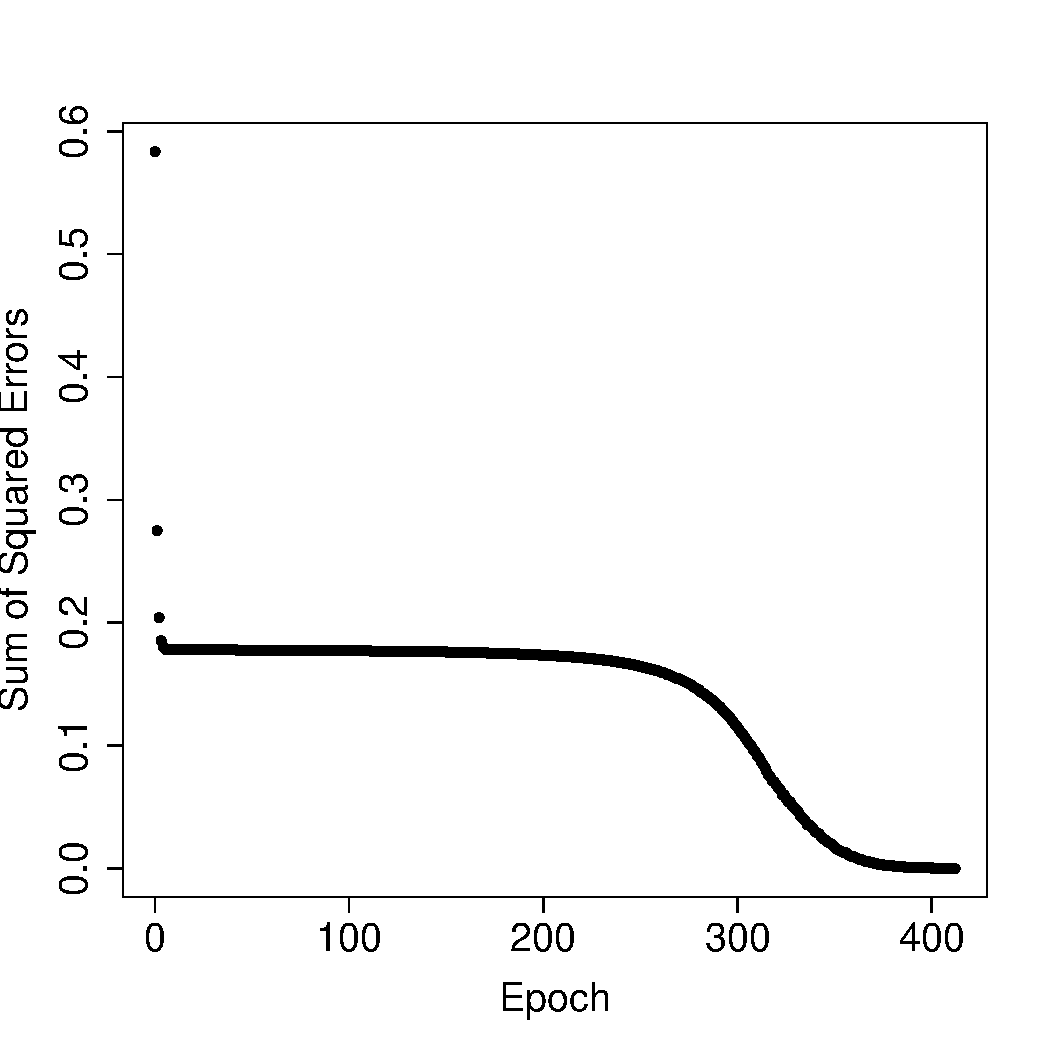
\includegraphics[width=0.5\textwidth]{./images/fmlpda_8_21.pdf}
}
\caption[A plot showing how the sum of squared errors of the ReLU network changed during training when $\alpha=0.1$.]{A plot showing how the sum of squared errors of the ReLU network changed during training when $\alpha=0.1$.}
\label{fig:SSEperTrainingIterationNNReLUAlpha01}
\end{figure}
\end{frame} 



 \begin{frame} 
\begin{equation}
	rectifier_{leaky}(z)=\begin{cases}
		z & \text{if } z > 0\\
		0.01\times z & otherwise
		\end{cases}
	\label{eqn:lrectifier}
\end{equation}
\begin{equation}
\frac{d}{dz} rectifier_{leaky}(z) = 	\begin{cases}
		1 & \text{if } z > 0\\
		0.01 & otherwise
	\end{cases}
	\label{eqn:lrectifierderivatve}
\end{equation}
\end{frame} 



 \begin{frame} 
\begin{equation}
	rectifier_{parametric}(z_i)=\begin{cases}
		z_i & \text{if } z_i > 0\\
		\lambda_i \times z_i & otherwise
		\end{cases}
	\label{eqn:prectifier}
\end{equation}
\begin{equation}
\frac{d}{dz} rectifier_{parametric}(z_i) = 	\begin{cases}
		1 & \text{if } z_i > 0\\
		\lambda_i & otherwise
	\end{cases}
	\label{eqn:prectifierderivatve}
\end{equation}
\end{frame} 



 \begin{frame} 
\begin{alignat}{5}
\frac{\partial \mathcal{E}}{\partial \lambda_{i}} &= \frac{\partial \mathcal{E}}{\partial a_i} &\times&  \frac{\partial a_i}{\partial \lambda_i}
\label{eq:errorgradientwithrespecttolambda}
\end{alignat}
\begin{equation}
\frac{\partial a_i}{\partial \lambda_i} = 	\begin{cases}
		0 & \text{if } z_i > 0\\
		z_i & otherwise
	\end{cases}
	\label{eqn:preluegradientwithrespecttolambda}
\end{equation}
\begin{equation}
\lambda_{i} \leftarrow \lambda_{i} - \alpha \times \frac{\partial \mathcal{E}}{\partial \lambda_{i}}
\label{eq:lambdaupdaterule}
\end{equation}
\end{frame} 

\subsection{Weight Initialization and Unstable Gradients}

 \begin{frame} 
\begin{alignat}{3}
\delta_i & = & 
	\underbrace{ w_{j,i} \times w_{k,j} \times }_{ \substack{\text{extreme weights}\\ \rightarrow \\\text{unstable gradients}}}
	\frac{\partial \mathcal{E}}{\partial a_k} 
	\underbrace{ \times \frac{\partial a_k}{\partial z_k} \times \frac{\partial a_j}{\partial z_j} \times \frac{\partial a_i}{\partial z_i} }_{\substack{\text{extreme weights}\\ \rightarrow \\ \text{saturated activations} \\ \rightarrow \\ \text{vanishing gradients}}}  
\label{eq:weightandunstablegradients}
\end{alignat}
\end{frame} 



 \begin{frame} 
\begin{figure}
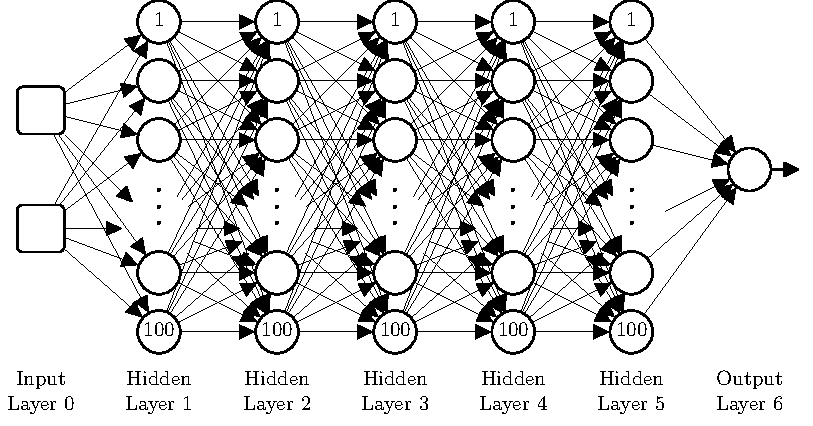
\includegraphics[width=\textwidth]{./images/fmlpda_8_22.pdf}
\caption{The architecture of the neural network used in the weight initialization experiments. Note that the neurons in this network use a linear activation function: $a_i=z_i$.}
\label{fig:weightinitarch}
\end{figure}
\end{frame} 



 \begin{frame} 
\begin{figure}
%\vspace{-1.2cm}
\centerline{
%{\setlength{\tabcolsep}{0.05em}
\begin{tabular}{cc}
	\subfigure[Weights by Layer]{\label{fig:Weight_Init_Standardized_Normal_Sigma_0_01_ws}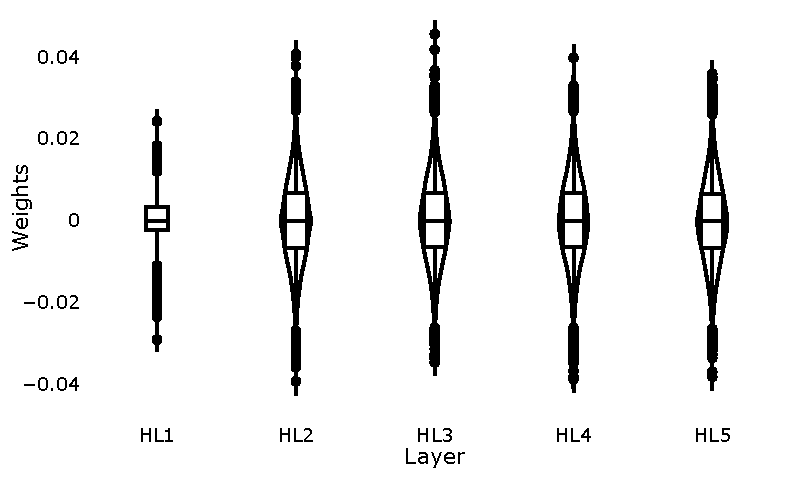
\includegraphics[width=0.42\textwidth]{./images/fmlpda_8_23_a.pdf}}&
	\subfigure[Weighted Sum ($z$) by Layer]{\label{fig:Weight_Init_Standardized_Normal_Sigma_0_01_zs}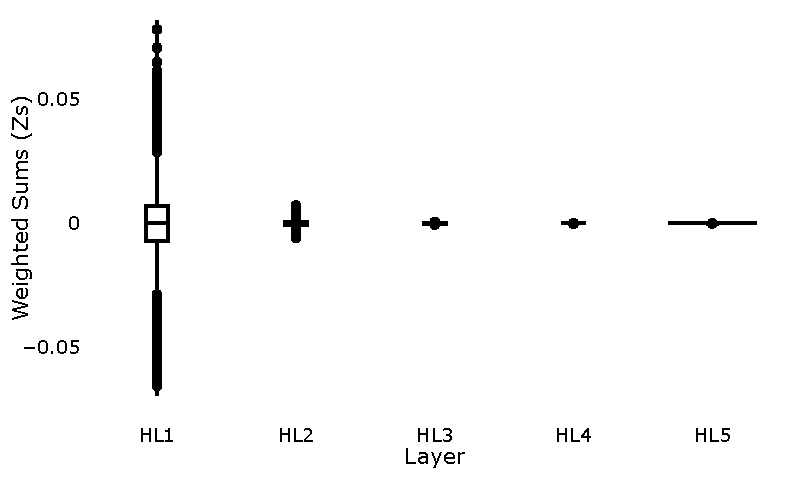
\includegraphics[width=0.42\textwidth]{./images/fmlpda_8_23_b.pdf}}\\
	\subfigure[Activations by Layer]{\label{fig:Weight_Init_Standardized_Normal_Sigma_0_01_as}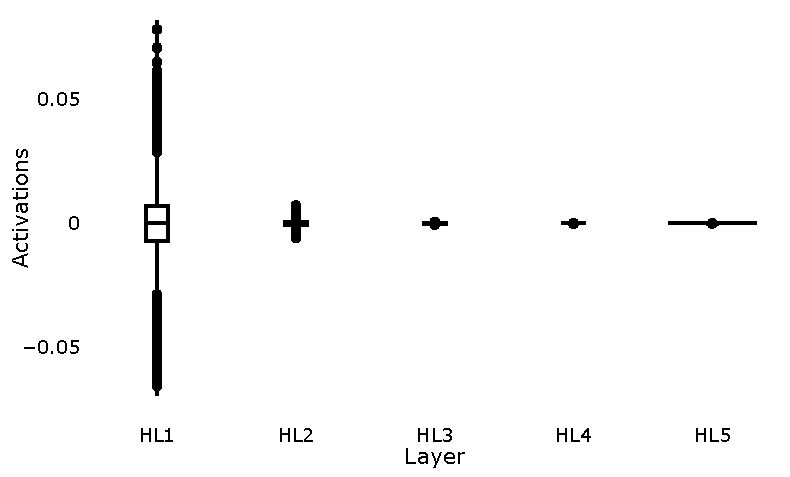
\includegraphics[width=0.42\textwidth]{./images/fmlpda_8_23_c.pdf}}&
	\subfigure[$\delta$s by Layer]{\label{fig:Weight_Init_Standardized_Normal_Sigma_0_01_ds}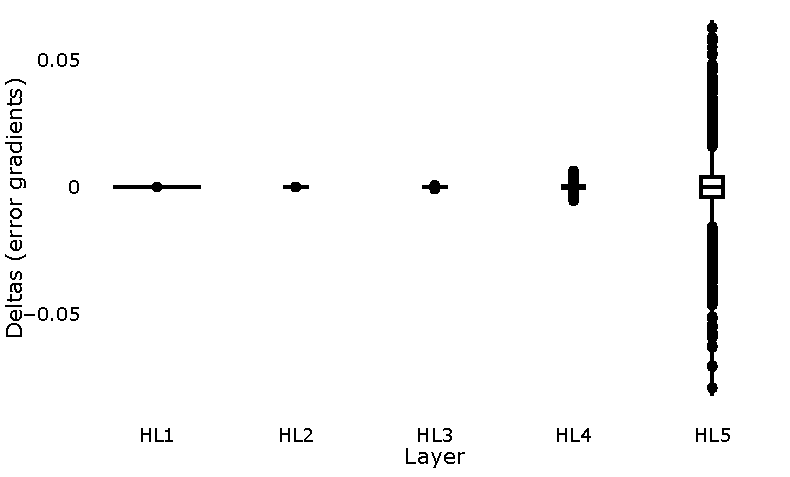
\includegraphics[width=0.42\textwidth]{./images/fmlpda_8_23_d.pdf}}
\end{tabular}
%}
}
\caption{The internal dynamics of the network in Figure \ourRef{fig:weightinitarch} during the first training iteration when the  weights were initialized using a normal distribution with $\mu{=}0.0, \sigma{=}0.01$.}
\label{fig:Weight_Init_Standardized_Normal_Sigma_0_01}
\end{figure}
\end{frame} 



 \begin{frame} 
\begin{figure}
%\vspace{-1.2cm}
\centerline{
%{\setlength{\tabcolsep}{0.05em}
\begin{tabular}{cc}
	\subfigure[Weights by Layer]{\label{fig:Weight_Init_Standardized_Normal_Sigma_0_2_ws}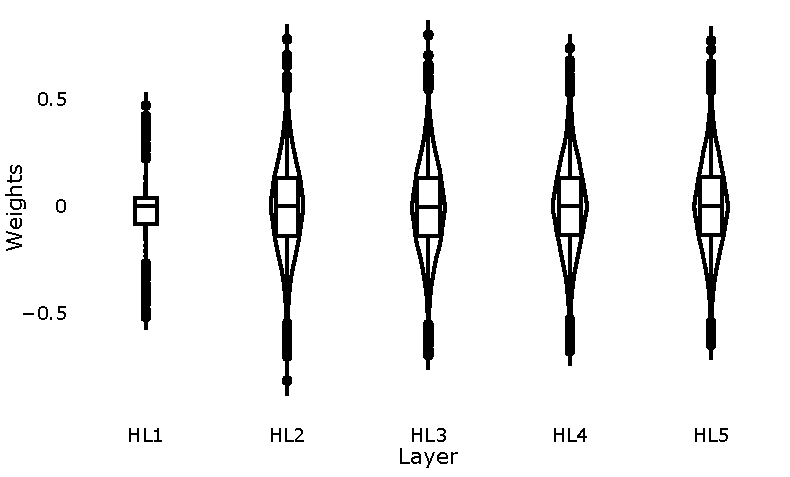
\includegraphics[width=0.42\textwidth]{./images/fmlpda_8_24_a.pdf}}&
	\subfigure[Weighted Sum ($z$) by Layer]{\label{fig:Weight_Init_Standardized_Normal_Sigma_0_2_zs}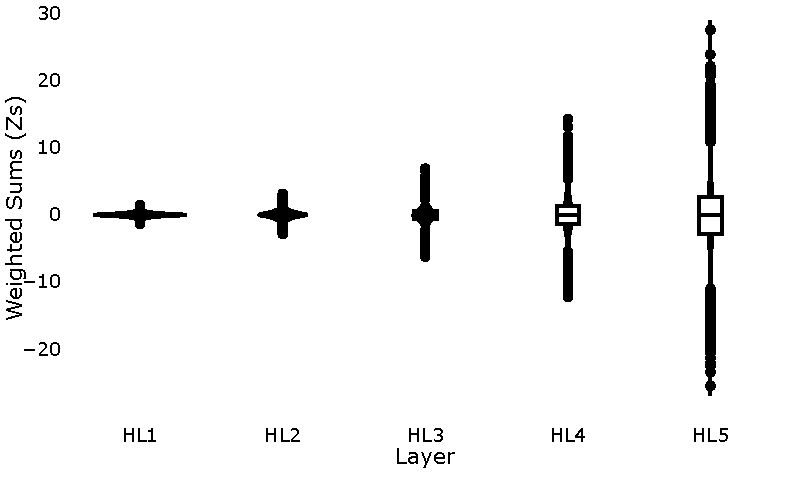
\includegraphics[width=0.42\textwidth]{./images/fmlpda_8_24_b.pdf}}\\
	\subfigure[Activations by Layer]{\label{fig:Weight_Init_Standardized_Normal_Sigma_0_2_as}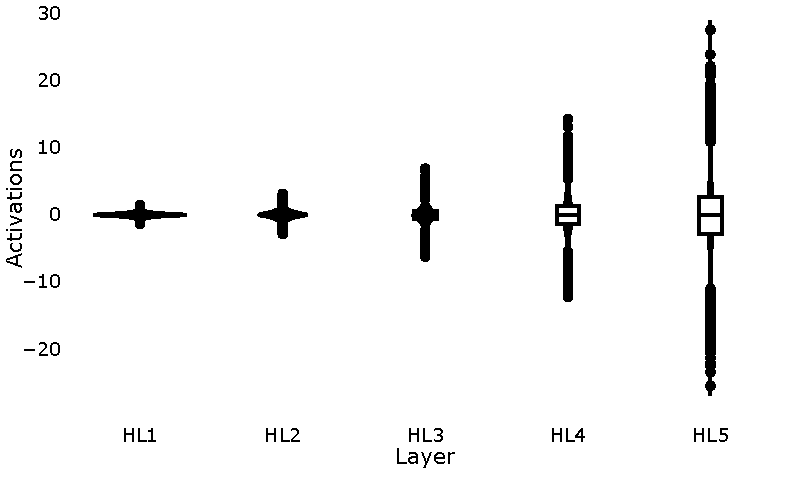
\includegraphics[width=0.42\textwidth]{./images/fmlpda_8_24_c.pdf}}&
	\subfigure[$\delta$s by Layer]{\label{fig:Weight_Init_Standardized_Normal_Sigma_0_2_ds}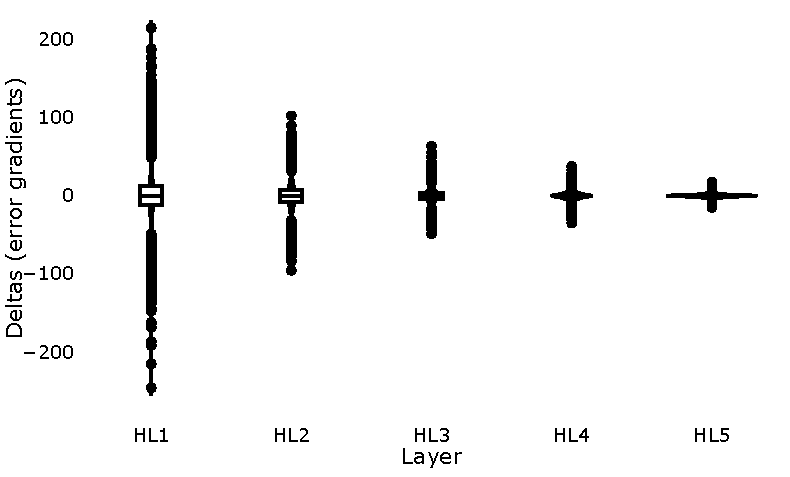
\includegraphics[width=0.42\textwidth]{./images/fmlpda_8_24_d.pdf}}
\end{tabular}
%}
}
\caption{The internal dynamics of the network in Figure \ourRef{fig:weightinitarch} during the first training iteration when the  weights were initialized using a normal distribution with $\mu=0.0$ and $\sigma=0.2$.}
\label{fig:Weight_Init_Standardized_Normal_Sigma_0_2}
\end{figure}
\end{frame} 



 \begin{frame} 
\begin{equation}
z= \left( w_1 \times  d_{1} \right) + \left( w_2 \times  d_{2} \right) + \dots + \left( w_{n_{in}} \times  d_{n_{in}} \right) 
\end{equation}
\end{frame} 



 \begin{frame} 
\begin{equation}
var\left( \sum_{i=1}^n X_i \right) = \sum_{i=1}^n var\left(X_i\right)
\label{eq:bienaymeformula}
\end{equation}
\end{frame} 



 \begin{frame} 
\begin{alignat}{1}
var(z)&= var\left(\left( w_1 \times  d_{1} \right) + \left( w_2 \times  d_{2} \right) + \dots \left( w_{n_{in}} \times  d_{n_{in}} \right) \right)\notag \\
&= \sum_{i=1}^{n_{in}} var(w_i \times d_{i})
\end{alignat}
\begin{equation}
var(w \times d) = \lbrack E(\textbf{W})\rbrack^2~var(\textbf{d}) + \lbrack E(\textbf{d})\rbrack^2~var(\mathbf{W}) + var(\mathbf{W})~var(\textbf{d})
\label{eq:varweightsinputs}
\end{equation}
\begin{equation}
var(w \times d) = var(\mathbf{W}) var(\textbf{d})
\end{equation}
\end{frame} 



 \begin{frame} 
\begin{equation}
var(z)= \sum_{i=1}^{n_{in}} var(w_i \times d_{i}) = n_{in}~var(\mathbf{W})~var(\textbf{d})
\label{eq:varz}
\end{equation}
\end{frame} 



 \begin{frame} 
\begin{alignat}{2}
var(Z^{(HL1)}) & =  n_{in}^{(HL1)} \times var(\mathbf{W}^{(HL1)}) \times var(\textbf{d}^{(HL1)})\\ \notag
& = 2 \times 0.0001 \times 1\\ \notag
& = 0.0002
\label{eq:varzexample}
\end{alignat}
\end{frame} 



 \begin{frame} 
\begin{alignat}{2}
var(Z^{(HL2)})& = n_{in}^{(HL2)} \times var(\mathbf{W}^{(HL2)}) \times var(\textbf{d}^{(HL2)})\\ \notag
& =  100 \times 0.0001 \times 0.0002\\ \notag
& = 0.000002
%\label{eq:varzexample2}
\end{alignat}
\end{frame} 



 \begin{frame} 
\begin{equation}
var(\mathbf{W}^{(k)})=\frac{2}{n_{in}^{(k)}+n_{out}^{(k)}}
\label{eq:xavierinout}
\end{equation}
\begin{equation}
var(\mathbf{W}^{(k)})=\frac{1}{n_{in}^{(k)}}
\label{eq:xavier}
\end{equation}
\end{frame} 



 \begin{frame} 
\begin{figure}
%\vspace{-1.2cm}
\centerline{
%{\setlength{\tabcolsep}{0.05em}
\begin{tabular}{cc}
	\subfigure[Weights by Layer]{\label{fig:Weight_Init_Standardized_Glorot_ws}
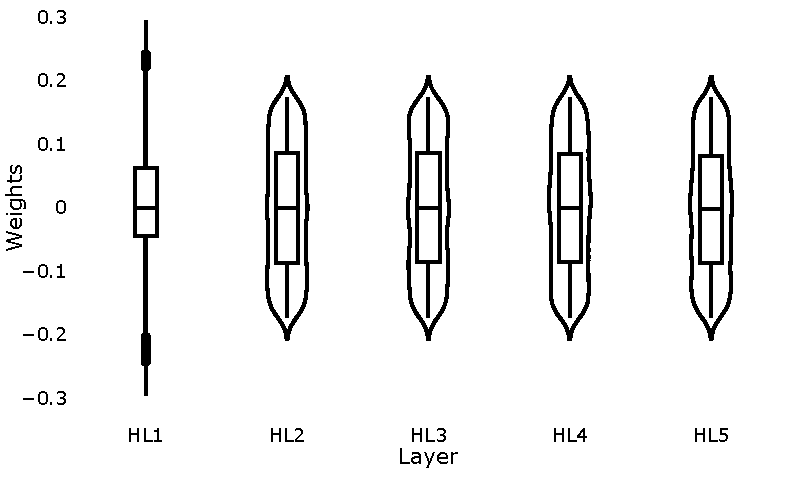
\includegraphics[width=0.42\textwidth]{./images/fmlpda_8_25_a.pdf}}&
	\subfigure[Weighted Sum ($z$) by Layer]{\label{fig:Weight_Init_Standardized_Glorot_zs}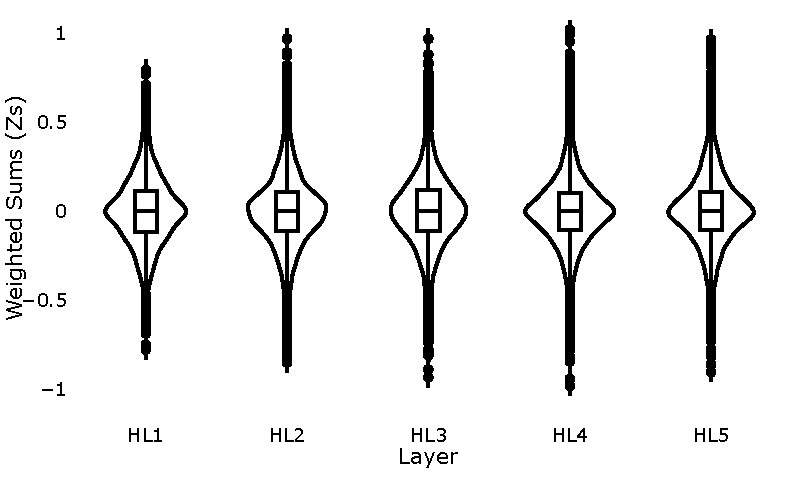
\includegraphics[width=0.42\textwidth]{./images/fmlpda_8_25_b.pdf}}\\
	\subfigure[Activations by Layer]{\label{fig:Weight_Init_Standardized_Glorot_as}
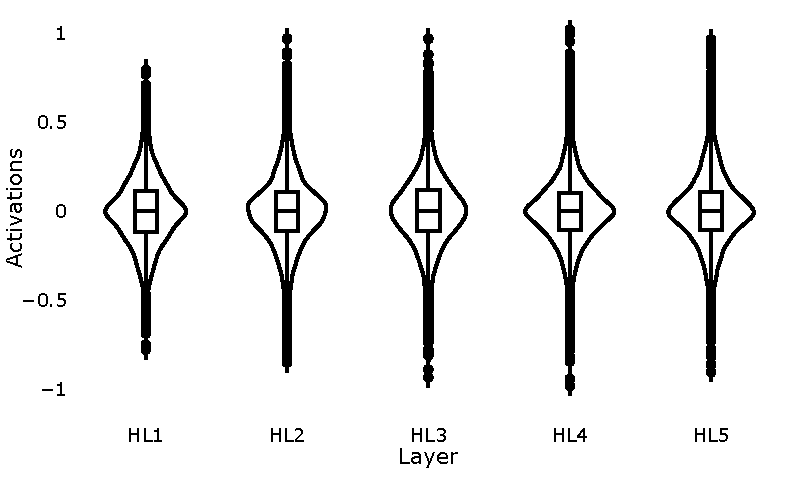
\includegraphics[width=0.42\textwidth]{./images/fmlpda_8_25_c.pdf}}&
	\subfigure[$\delta$s by Layer]{\label{fig:Weight_Init_Standardized_Glorot_ds}
	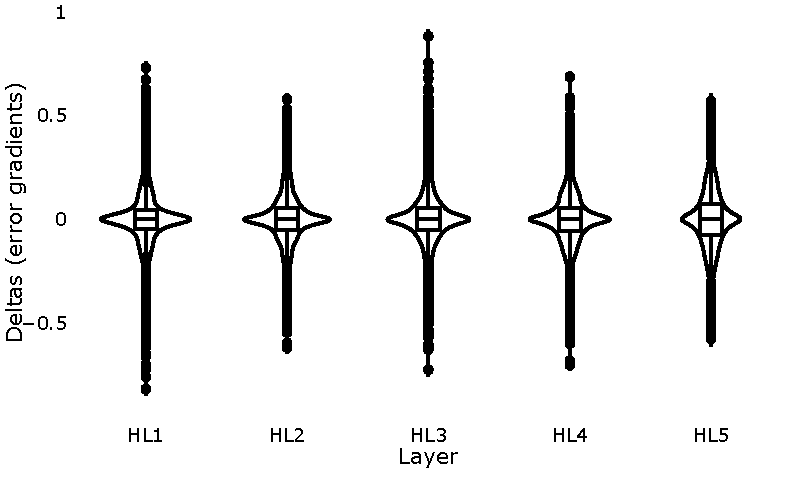
\includegraphics[width=0.42\textwidth]{./images/fmlpda_8_25_d.pdf}}
\end{tabular}
%}
}
\caption{The internal dynamics of the network in Figure \ourRef{fig:weightinitarch} during the first training iteration when the  weights were initialized using Xavier initialization.}
\label{fig:Weight_Init_Standardized_Glorot}
\end{figure}
\end{frame} 



 \begin{frame} 
\begin{equation}
var(\mathbf{W}^{(k)})=\frac{2}{n_{in}^{(k)}}
\label{eq:kaiming}
\end{equation}
\end{frame} 



 \begin{frame} 
\begin{alignat}{3}
W^{(1)}  & \thicksim & \mathcal{N}\left(0, \sqrt{\frac{1}{100}}\right) \notag\\
W^{(2)}  & \thicksim & \mathcal{N}\left(0, \sqrt{\frac{2}{80}}\right) \notag\\
W^{(3)}  & \thicksim & \mathcal{N}\left(0, \sqrt{\frac{2}{50}}\right) 
\label{eq:3layerweightinit}
\end{alignat}
\end{frame} 



 \begin{frame} 
\begin{figure}
%\vspace{-1.2cm}
\centerline{
%{\setlength{\tabcolsep}{0.05em}
\begin{tabular}{cc}
	\subfigure[Weights by Layer]{\label{fig:Weight_Init_Standardized_ReLU_He_ws}
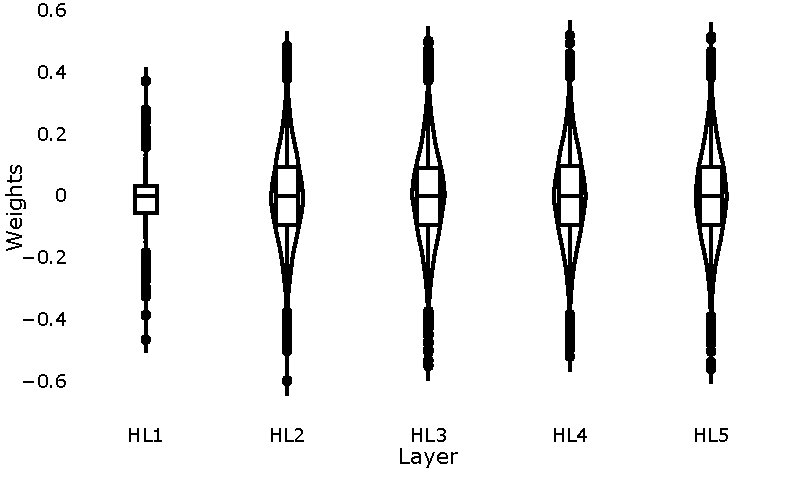
\includegraphics[width=0.43\textwidth]{./images/fmlpda_8_26_a.pdf}}&
	\subfigure[Weighted Sum ($z$) by Layer]{\label{fig:Weight_Init_Standardized_ReLU_He_zs}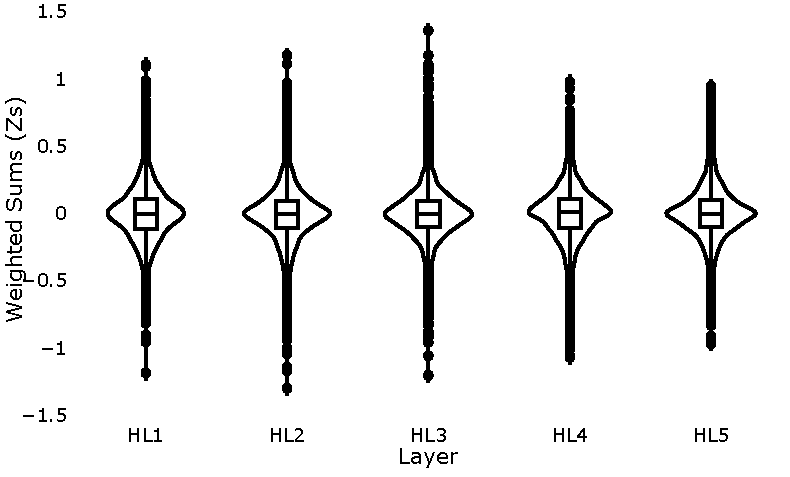
\includegraphics[width=0.43\textwidth]{./images/fmlpda_8_26_b.pdf}}\\
	\subfigure[Activations by Layer]{\label{fig:Weight_Init_Standardized_ReLU_He_as}
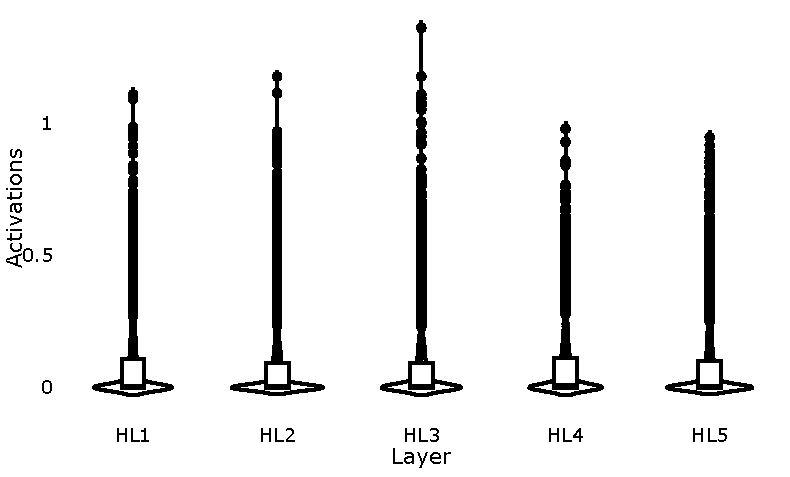
\includegraphics[width=0.42\textwidth]{./images/fmlpda_8_26_c.pdf}}&
	\subfigure[$\delta$s by Layer]{\label{fig:Weight_Init_Standardized_ReLU_He_ds}
	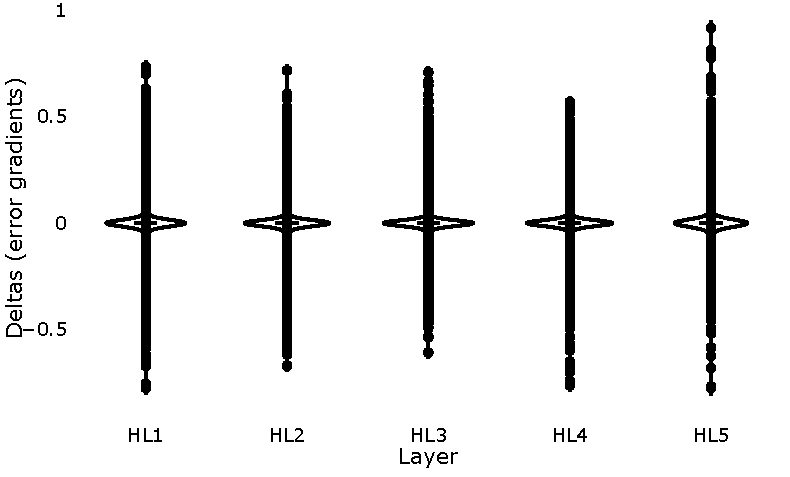
\includegraphics[width=0.42\textwidth]{./images/fmlpda_8_26_d.pdf}}
\end{tabular}
}
%}
\caption{The internal dynamics of the network in Figure \ourRef{fig:weightinitarch}, using ReLUs, during the first training iteration when the weights were initialized using He initialization.}
\label{fig:Weight_Init_Standardized_He}
\end{figure}
\end{frame} 


\subsection{Handling Categorical Target Features: Softmax Output Layers and Cross-Entropy Loss Functions}

\begin{frame}
\begin{enumerate}
	\item represent the target feature using \keyword{one-hot encoding};
	\item change the output layer of the network to be a \keywordAlias{softmax layer}{softmax output layer}; and
	\item change the error (or loss) function we use for training to be the \keyword{cross-entropy} function.
\end{enumerate}
\end{frame}

 \begin{frame} 
\begin{table}
\caption{The \emph{range-normalized} hourly samples of ambient factors and full load electrical power output of a combined cycle power plant, rounded to two decimal places, and with the (binned) target feature represented using one-hot encoding.}
\label{tab:onehostnormalizedpowerplandata}
\noindent\resizebox{\textwidth}{!}{
\begin{tabular}{cccccc}
\hline
\featN{ID} & \featN{Ambient Temperature} & \featN{Relative Humidity} & \multicolumn{3}{c}{Electrical Output}\\
~ & $^\circ$C & \% & \featL{low} & \featL{medium} & \featL{high}\\
\hline
1 & 0.04 & 0.81 & 0 & 0 & 1\\
2 & 0.84 & 0.58 & 1 & 0 & 0\\
3 & 0.50 & 0.07 & 0 & 1 & 0\\
4 & 0.53 & 1.00 & 0 & 1 & 0\\
\hline
\end{tabular}
}
\end{table}
\end{frame} 



 \begin{frame} 
\begin{equation}
\varphi_{sm}\left(z_i\right)=\frac{e^{z_i}}{\sum_{j=1}^{m} e^{z_m}}
\label{eq:softmaxfunc}
\end{equation}
\end{frame} 



 \begin{frame}[plain]
\begin{table}
\caption[The calculation of the softmax activation function $\varphi_{sm}$ over a vector of three logits $\mathbf{l}$.]{The calculation of the softmax activation function $\varphi_{sm}$ over a vector of three logits $\mathbf{l}$.}
\label{tab:softmax}
%\noindent\resizebox{\textwidth}{!}{
\begin{tabular}{lrrr}
\hline
~  & $\mathbf{l}_0$ & $\mathbf{l}_1$ & $\mathbf{l}_2$ \\ 
\hline
\featN{$\mathbf{l}$} & 1.5 & -0.9 & 0.6\\
\featN{$e^{\mathbf{l}_i}$} & 4.48168907 & 0.40656966 & 1.8221188\\
\featN{$\sum_{i}e^{\mathbf{l}_i}$} & ~ & ~ & 6.71037753\\
\featN{$\varphi_{sm}(\mathbf{l}_i)$} & 0.667874356 & 0.060588195 & 0.27153745\\
\hline
\end{tabular}
%}
\end{table}
\end{frame} 



 \begin{frame} 
\begin{figure}[t]
\centerline{
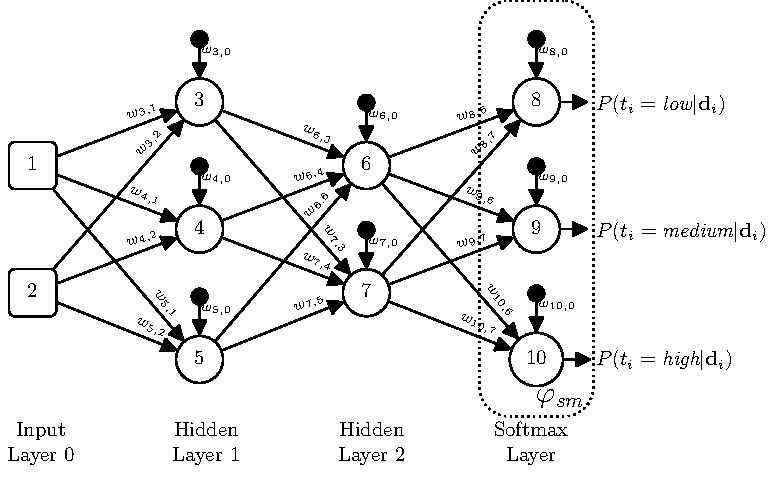
\includegraphics[width=\textwidth]{./images/fmlpda_8_27.pdf}
}
\caption[A schematic of a feedforward artificial neural network with a three-neuron softmax output layer.]{A schematic of a feedforward artificial neural network with a three-neuron softmax output layer.}
\label{fig:nn-softmax-output}
\end{figure}
\end{frame} 



 \begin{frame} 
\begin{equation}
L_{CE}\left(\mathbf{t}, \mathbf{\hat{P}}\right) = - \sum_j \mathbf{t}_j \ln \left(\mathbf{\hat{P}}_j \right)
\label{eq:crossentropy}
\end{equation}
\begin{equation}
L_{CE}\left(\mathbf{t}, \mathbf{\hat{P}}\right) = - \ln \left(\mathbf{\hat{P}}_\star \right)
\label{eq:crossentropyonehot}
\end{equation}
\end{frame} 



 \begin{frame} 
\begin{alignat}{5}
L_{CE}\left(\mathbf{t}, \mathbf{\hat{P}}\right) & = - \sum_j \mathbf{t}_j \ln \left(\mathbf{\hat{P}} _j \right) \notag\\
~ & = - \left( \left( \mathbf{t}_0 \ln \left(\mathbf{\hat{P}} _0 \right) \right) +  \left( \mathbf{t}_1 \ln \left(\mathbf{\hat{P}} _1 \right) \right) + \left( \mathbf{t}_2 \ln \left(\mathbf{\hat{P}} _2 \right) \right) \right)\notag\\
~ & = - \left(  \left( 0 \ln \left(\mathbf{\hat{P}} _0 \right) \right) +  \left( 1 \ln \left(\mathbf{\hat{P}} _1 \right) \right) +  \left( 0 \ln \left(\mathbf{\hat{P}} _2 \right) \right) \right)\notag\\
~ & = -  1 \ln \left(\mathbf{\hat{P}} _1 \right) 
\label{eq:simplifiyingcrossentropy}
\end{alignat}
\end{frame} 



 \begin{frame} 
\begin{alignat}{1}
\boldsymbol{\delta}_k&= \frac{\partial \mathcal{E}}{\partial z_k} \label{eq:chainCEdefStep1}\\
~&= \frac{\partial L_{CE}\left(\mathbf{t}, \mathbf{\hat{P}}\right)}{\partial \mathbf{l}_k} \label{eq:chainCEdefStep2}\\
~&= \frac{\partial - \ln \left(\mathbf{\hat{P}}_\star \right) }{\partial \mathbf{l}_k} \label{eq:chainCEdefStep3}\\
~&= \frac{\partial - \ln \left(\mathbf{\hat{P}}_\star \right) }{\partial \left(\mathbf{\hat{P}}_\star \right)} \times \frac{\partial \left(\mathbf{\hat{P}}_\star \right)}{\partial \mathbf{l}_k} \label{eq:chainCEdefStep4}
\end{alignat}
\end{frame} 



 \begin{frame} 
\begin{equation}
\frac{d \ln x}{d x} = \frac{1}{x}
\end{equation}
\begin{equation}
\frac{\partial - \ln \left(\mathbf{\hat{P}}_\star \right) }{\partial \left(\mathbf{\hat{P}}_\star \right)} = -\frac{1}{\mathbf{\hat{P}}_\star}
\label{eq:derivativeofneglogprob}
\end{equation}
\begin{equation}
\frac{\partial \left(\mathbf{\hat{P}}_\star \right)}{\partial \mathbf{l}_k} = 	\begin{cases}
		 \mathbf{\hat{P}}_\star  \left(1-\mathbf{\hat{P}}_k \right) & \text{if}~k = \star \\
		- \mathbf{\hat{P}}_\star  \mathbf{\hat{P}}_k & otherwise
		\end{cases}
\label{eq:softmaxderivative}
\end{equation}
\end{frame} 



 \begin{frame} 
\begin{alignat}{3}
\boldsymbol{\delta}_k&= \frac{\partial - \ln \left(\mathbf{\hat{P}}_\star \right) }{\partial \left(\mathbf{\hat{P}}_\star \right)} & \times & \frac{\partial \left(\mathbf{\hat{P}}_\star \right)}{\partial \mathbf{l}_k} \label{eq:chainCEdefStep5}\\
~ &= ~~~~-\frac{1}{\mathbf{\hat{P}}_\star} & \times & \frac{\partial \left(\mathbf{\hat{P}}_\star \right)}{\partial \mathbf{l}_k} \label{eq:chainCEdefStep6}\\
~ &= ~~~~-\frac{1}{\mathbf{\hat{P}}_\star} & \times & \begin{cases}
		 \mathbf{\hat{P}}_\star  \left(1-\mathbf{\hat{P}}_k \right) & \text{if}~k = \star \\
		- \mathbf{\hat{P}}_\star  \mathbf{\hat{P}}_k & otherwise
		\end{cases} \label{eq:chainCEdefStep7}\\
~ &= && \begin{cases}
		 - \left(1-\mathbf{\hat{P}}_k \right) & \text{if}~k = \star \\
		\mathbf{\hat{P}}_k & otherwise
		\end{cases}  \label{eq:chainCEdefStep8}
\end{alignat}
\end{frame} 



 \begin{frame} 
\begin{equation}
\boldsymbol{\delta}_{k=\star}=- \left(1-\mathbf{\hat{P}}_k \right)
\label{eq:catdeltastar}
\end{equation}
\begin{equation}
\boldsymbol{\delta}_{k\neq\star}= \mathbf{\hat{P}}_k
\label{eq:catdeltaNOTstar}
\end{equation}
\end{frame} 



 \begin{frame} 
\begin{figure}
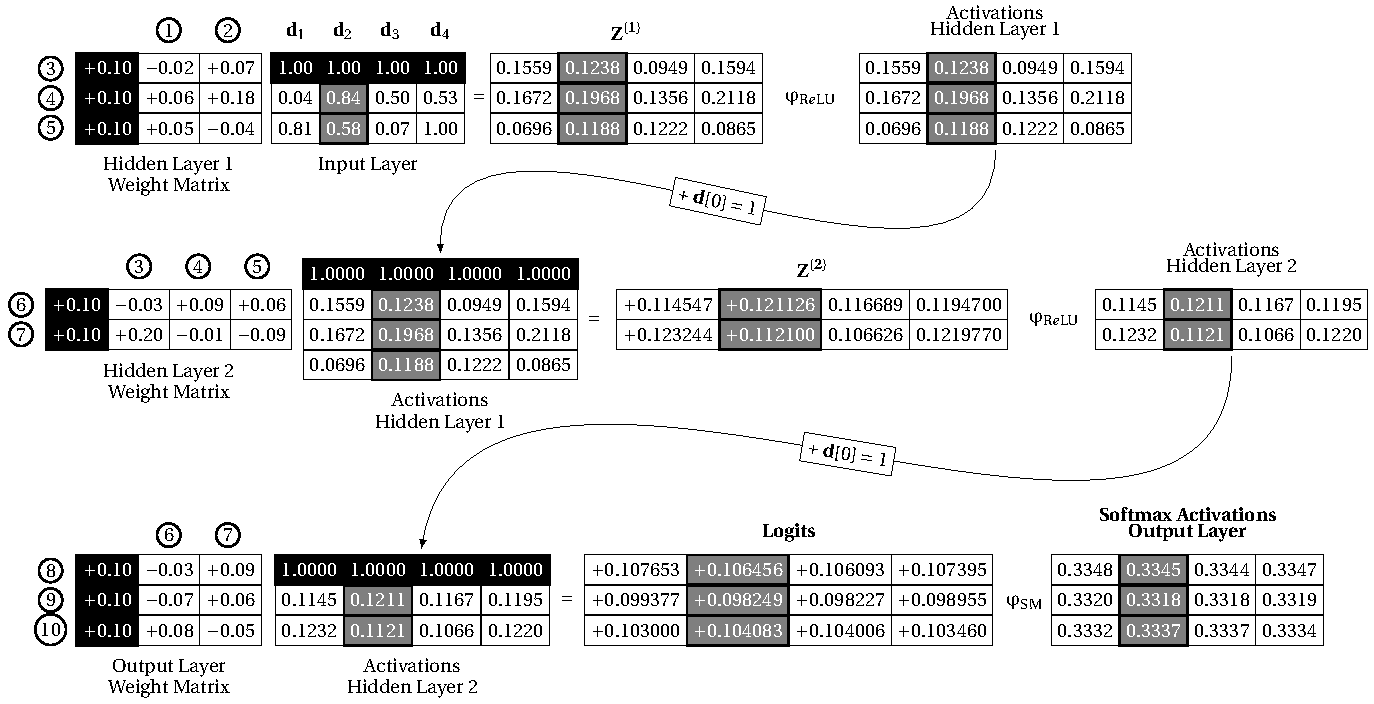
\includegraphics[width=\textwidth]{./images/fmlpda_8_28.pdf}
\caption{The forward pass of the mini-batch of examples listed in Table \ourRef{tab:onehostnormalizedpowerplandata} through the network in Figure \ourRef{fig:nn-softmax-output}.}
\label{fig:ReluCatForwardPass}
\end{figure}
\end{frame} 



 \begin{frame}[plain]
\begin{table}[!t]
\caption {The calculation of the softmax activations for each of the neurons in the output layer for each example in the mini-batch, and the calculation of the $\delta$ for each neuron in the output layer for each example in the mini-batch.}
\label{tab:softmaxanddeltas}
%{\setlength{\tabcolsep}{0.1em}
%\begin{tabular*}{\linewidth}{@{\extracolsep{\fill}} lrrrr @{}}
\noindent\resizebox{0.8\textwidth}{!}{
\begin{tabular}{lrrrr}
\hline
~ & $\mathbf{d}_1$ & $\mathbf{d}_2$ & $\mathbf{d}_3$ & $\mathbf{d}_4$ \\ 
\hline
\multicolumn{5}{l}{Per Neuron Per Example logits}\\
Neuron 8 &  0.107653 & 0.106456 & 0.106093 & 0.107395 \\
Neuron 9 &  0.099377 & 0.098249 & 0.098227 & 0.098955 \\
Neuron 10 &  0.103000 & 	0.104083 & 0.1040060 &0.103460 \\
\hline
\multicolumn{5}{l}{Per Neuron Per Example $e^{\mathbf{l}_i}$}\\
Neuron 8 & 1.113661238 & 1.112328983 & 1.111925281 & 1.11337395\\
Neuron 9 & 1.104482611 & 1.103237457 & 1.103213186 & 1.104016618\\
Neuron 10 & 1.108491409 & 1.109692556 & 1.109607113 & 1.109001432\\
$\sum_i e^{\mathbf{l}_i}$ & 3.326635258 & 3.325258996 & 3.324745579 & 3.326392\\
\hline
\multicolumn{5}{l}{Per Neuron Per Example Softmax Activations}\\
Neuron 8 & 0.3348 & 0.3345 & 0.3344 & 0.3347\\
Neuron 9 & 0.3320 & 0.3318 & 0.3318 & 0.3319\\
Neuron 10 & 0.3332 & 0.3337 & 0.3337 & 0.3334\\
\hline
\multicolumn{5}{l}{Per Neuron Target One-Hot Encodings}\\
Neuron 8 & 0 & 1 & 0 & 0\\
Neuron 9 & 0 & 0 & 1 & 1\\
Neuron 10 & 1 & 0 & 0 & 0\\
\hline
\multicolumn{5}{l}{Per Neuron Per Example $\delta$s}\\
Neuron 8 & 0.3348 & -0.6655 & 0.3344 & 0.3347\\
Neuron 9 & 0.3320 & 0.3318 & -0.6682 & -0.6681\\
Neuron 10	 & -0.6668	 & 0.3337 & 0.3337 & 0.3334\\
\hline
\end{tabular}
}
%\end{tabular*}
%}
\end{table}
\end{frame} 



 \begin{frame} 
\begin{alignat}{2}
\Delta w_{9,6} &= \sum_{j=1}^4 \boldsymbol{\delta}_{9,j} \times  a_{6,j} \notag\\
~ &= \left(0.3320 \times  0.1145\right) + \left(0.3318 \times  0.1211\right) \notag\\
~&\quad+ \left(-0.6682 \times  0.1167\right) + \left(-0.6681 \times  0.1195\right)  \notag\\
~ & = 0.038014 + 0.04018098 + -0.07797894 + -0.07983795 \notag\\
~ & = -0.07962191
\label{eq:w96BathDelta}
\end{alignat}
\end{frame} 



 \begin{frame} 
\begin{alignat}{2}
w_{9,6} &= w_{9,6} - \alpha \times \Delta w_{9,6} \notag\\
~ &= -0.07 - 0.01\times -0.07962191 \notag\\
~ & = -0.07 - \left(-0.000796219 \right) \notag\\
~ & = -0.069203781
\label{eqn:w96weightupdate}
\end{alignat}
\end{frame} 

\subsection{Early Stopping and Dropout: Preventing Overfitting}

\begin{frame}[plain]
\begin{algorithm}[H]
\tiny
\caption[The early stopping algorithm]{The early stopping algorithm}
\begin{algorithmic}[1]
\Require $p$ the patience parameter 
\Require $\mathcal{D}_\nu$ a validation set
\State bestValidationError $=\infty$
\State tmpValidationError $=0$
\State $\theta=$ initial model parameters
\State $\theta^{best}=0$
\State patienceCount = 0

\While{patienceCount $< p$}
	\State $\theta=$ new model parameters after most recent weight update
	\State tmpValidationError = calculateValidationError($\theta$, $\mathcal{D}_\nu$)
	\If{bestValidationError $\geq$ tmpValidationError}
		\State bestValidationError = tmpValidationError
		\State  $\theta^{best}=\theta$
		\State patienceCount = 0
	\Else
		\State patienceCount = patienceCount + 1
	\EndIf
\EndWhile
\State \Return Best Model Parameters $\theta^{best}$
\end{algorithmic}
\label{alg:earlystopping}
\end{algorithm}
\end{frame}


 \begin{frame} 
\begin{figure}[t]
\centerline{
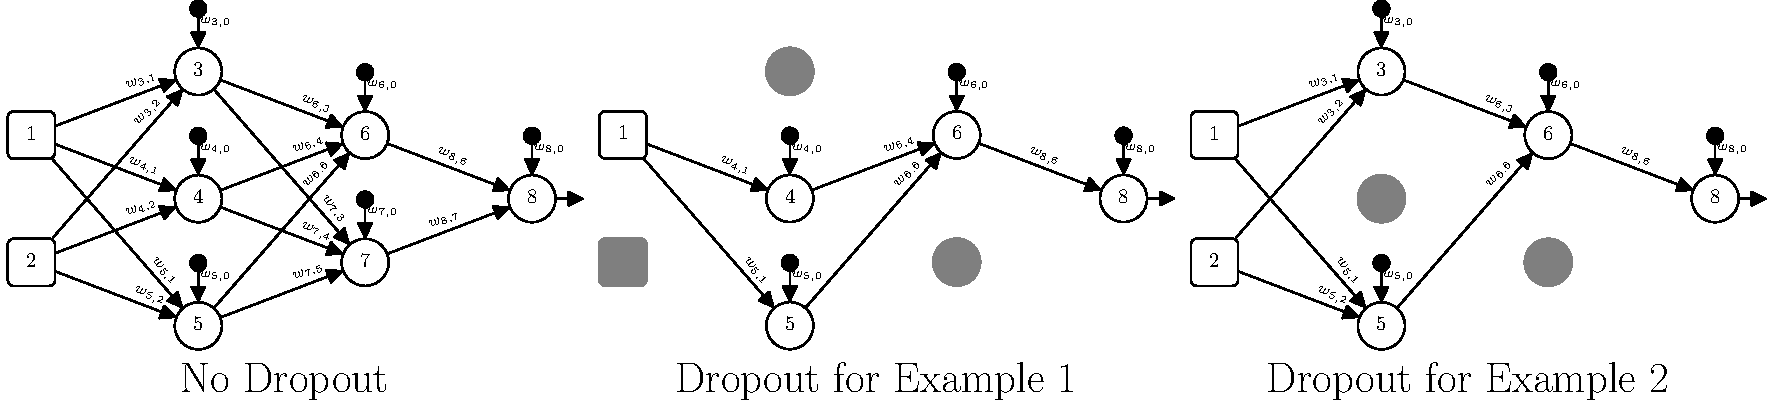
\includegraphics[width=\linewidth]{./images/fmlpda_8_29.pdf}
}
\caption[An illustration of how different small networks are generated for different training examples by applying dropout to the original large network.]{An illustration of how different small networks are generated for different training examples by applying dropout to the original large network. The gray nodes mark the neurons that have been dropped from the network for the training example.}
\label{fig:dropout}
\end{figure}
\end{frame} 

\begin{frame}[plain]
\begin{algorithm}[H]
\tiny
\caption[Extensions to Backpropagation to Use Inverted Dropout]{Extensions to Backpropagation to Use Inverted Dropout}
\begin{algorithmic}[1]
\Require $\rho$ probability that a neuron in a layer will not be dropped

\Comment{Forward Pass}
\For{each input or hidden layer $l$}
	\State $\mathbf{DropMask}^{(l)} = (m_1, \dots, m_{size(l)}) \sim Bernoulli(\rho)$ \label{line:vectorsample}
	\State $\mathbf{a}^{(l)'} = \mathbf{a}^{(l)} \odot \mathbf{DropMax}^{(l)}$ \label{line:masking}
	\State $\mathbf{a}^{(l)''} = \frac{1}{\rho} \mathbf{a}^{(l)'}$ \label{line:scaling}
\EndFor

\Comment{Backward Pass}
\For{each layer $l$ in backward pass}
	\State $\mathbf{\delta}^{(l)}=\mathbf{\delta}^{(l)} \odot \mathbf{DropMax}^{(l)}$ \label{line:setdeltatozero}
%	\For{each neuron $i$ in $l$}
%		\State $\delta_i'=\delta_i \times \mathbf{DropMax}^{(l)}$ \label{line:setdeltatozero}
%	\EndFor
\EndFor
\end{algorithmic}
\label{alg:dropout}
\end{algorithm}
\end{frame}

\subsection{Convolutional Neural Networks}

 \begin{frame} 
\begin{figure}[t]
\centerline{
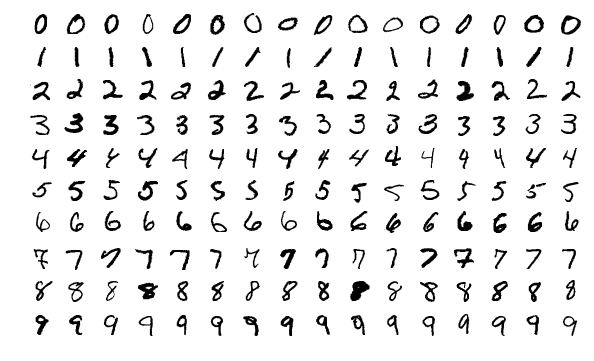
\includegraphics[width=0.9\textwidth]{./images/fmlpda_8_30.png}
}
\caption[Samples of the handwritten digit images from the MNIST dataset.]{Samples of the handwritten digit images from the MNIST dataset. Image attribution: Josef Steppan, used here under the Creative Commons Attribution-Share Alike 4.0 International license \url{https://creativecommons.org/licenses/by-sa/4.0)} and was sourced via Wikimedia Commons \url{https://commons.wikimedia.org/wiki/File:MnistExamples.png}.}
\label{fig:mnistsamples}
\end{figure}
\end{frame} 



 \begin{frame} 
\begin{equation}
\begin{bmatrix}
000 & 000 & 000 & 000 & 000 & 000\\
000 & \mathbf{255} & 000 & 000 & 000 & 000\\
000 & \mathbf{255} & 000 & \mathbf{255} & 000 & 000\\
000 & \mathbf{255} & \mathbf{255} & \mathbf{255} & \mathbf{255} & 000\\
000 & 000 & 000 & \mathbf{255} & 000 & 000\\
000 & 000 & 000 & 000 & 000 & 000\\
\end{bmatrix}
\label{eq:digit4matrix}
\end{equation}
\end{frame} 


\subsubsection{Local receptive fields and filters}

 \begin{frame} 
\begin{figure}[t]
\centerline{
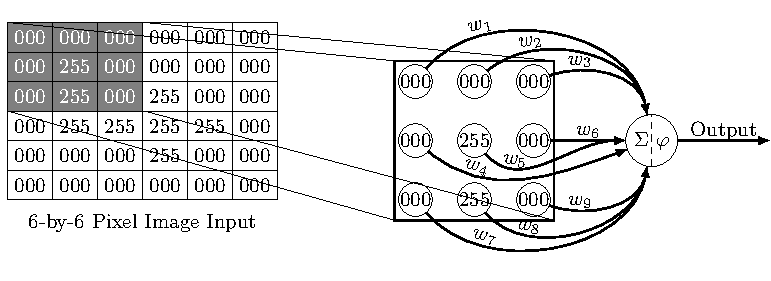
\includegraphics[width=\textwidth]{./images/fmlpda_8_31.pdf}
}
\caption[A 6-by-6 matrix representation of a grayscale image of a 4, and a neuron with a receptive field that covers the top-left corner of the image.]{A 6-by-6 matrix representation of a grayscale image of a 4, and a neuron with a receptive field that covers the top-left corner of the image. This figure was inspired by Figure 2 of \citep{kelleher2017not}.}
\label{fig:cnn-layer1-receptivefield}
\end{figure}
\end{frame} 



 \begin{frame} 
\begin{equation}
\begin{bmatrix}
0 & 0 & 0\\
1 & 1 & 1\\
0 & 0 & 0\\
\end{bmatrix}
\label{eq:filterexample1}
\end{equation}
\begin{alignat}{2}
a_i&= rectifier(\left(w_1 \times 000\right) + \left(w_2 \times 000\right) + \left(w_3 \times 000\right)\notag\\
~&\hspace{1.45cm}+\left(w_4 \times 000\right) + \left(w_5 \times 255\right) + \left(w_6 \times 000\right)\notag\\
~&\hspace{1.45cm}+\left(w_7 \times 000\right) + \left(w_8 \times 255\right) + \left(w_9 \times 000\right) )\notag\\
~&= rectifier(\left(0 \times 000\right) + \left(0 \times 000\right) + \left(0 \times 000\right)\notag\\
~&\hspace{1.45cm}+\left(1 \times 000\right) + \left(1 \times 255\right) + \left(1 \times 000\right)\notag\\
~&\hspace{1.45cm}+\left(0 \times 000\right) + \left(0 \times 255\right) + \left(0 \times 000\right) )\notag\\
~&= 255~
\label{eq:activationreceptivefield1}
\end{alignat}
\end{frame} 



 \begin{frame} 
\begin{figure}[t]
\centerline{
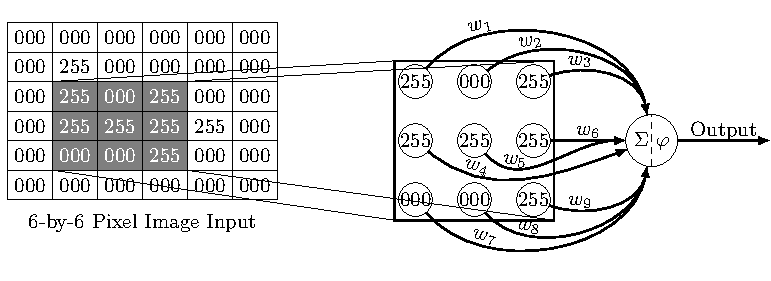
\includegraphics[width=\textwidth]{./images/fmlpda_8_32.pdf}
}
\caption[A 6-by-6 matrix representation of a grayscale image of a 4, and a neuron with a different receptive field from the neuron in Figure \ourRef{fig:cnn-layer1-receptivefield}.]{A 6-by-6 matrix representation of a grayscale image of a 4, and a neuron with a different receptive field from the neuron in Figure \ourRef{fig:cnn-layer1-receptivefield}. This figure was inspired by Figure 2 of \citep{kelleher2017not}.}
\label{fig:cnn-layer1-receptivefield2}
\end{figure}
\end{frame} 



 \begin{frame} 
\begin{alignat}{2}
a_i&= rectifier(\left(w_1 \times 255\right) + \left(w_2 \times 000\right) + \left(w_3 \times 255\right)\notag\\
~&\hspace{1.45cm}+\left(w_4 \times 255\right) + \left(w_5 \times 255\right) + \left(w_6 \times 255\right)\notag\\
~&\hspace{1.45cm}+\left(w_7 \times 000\right) + \left(w_8 \times 000\right) + \left(w_9 \times 255\right) )\notag\\
~&= rectifier(\left(0 \times 255\right) + \left(0 \times 000\right) + \left(0 \times 255\right)\notag\\
~&\hspace{1.45cm}+ \left(1 \times 255\right) + \left(1 \times 255\right) + \left(1 \times 255\right)\notag\\
~&\hspace{1.45cm}+ \left(0 \times 000\right) + \left(0 \times 000\right) + \left(0 \times 255\right) )\notag\\
~&= 765~
\label{eq:activationreceptivefield2}
\end{alignat}
\end{frame} 



 \begin{frame} 
\begin{alignat}{2}
\begin{bmatrix}
0 & 1 & 0\\
0 & 1 & 0\\
0 & 1 & 0\\
\end{bmatrix}
&\quad
\begin{bmatrix}
1 & 0 & 0\\
0 & 1 & 0\\
0 & 0 & 1\\
\end{bmatrix}
&\quad
\begin{bmatrix}
-1 & +1 & -1\\
-1 & +1 & -1\\
-1 & +1 & -1\\
\end{bmatrix}
&\quad
\begin{bmatrix}
-1 & -1 & -1\\
+1 & +1 & +1\\
-1 & -1 & -1\\
\end{bmatrix}
\label{eq:3filterexamples}
\end{alignat}
\end{frame} 

\subsubsection{Weight sharing and translation equivariant feature detection}

 \begin{frame} 
\begin{alignat}{2}
\Delta w_{i,*} &= \sum_{i=1}^m \boldsymbol{\delta}_i \times  a_* \notag \\
w_{i,*} &\leftarrow w_{i,*} - \alpha \times \Delta w_{i,*}
\label{eqn:filterweightupdaterule}
\end{alignat}
\end{frame} 



 \begin{frame} 
\begin{figure}
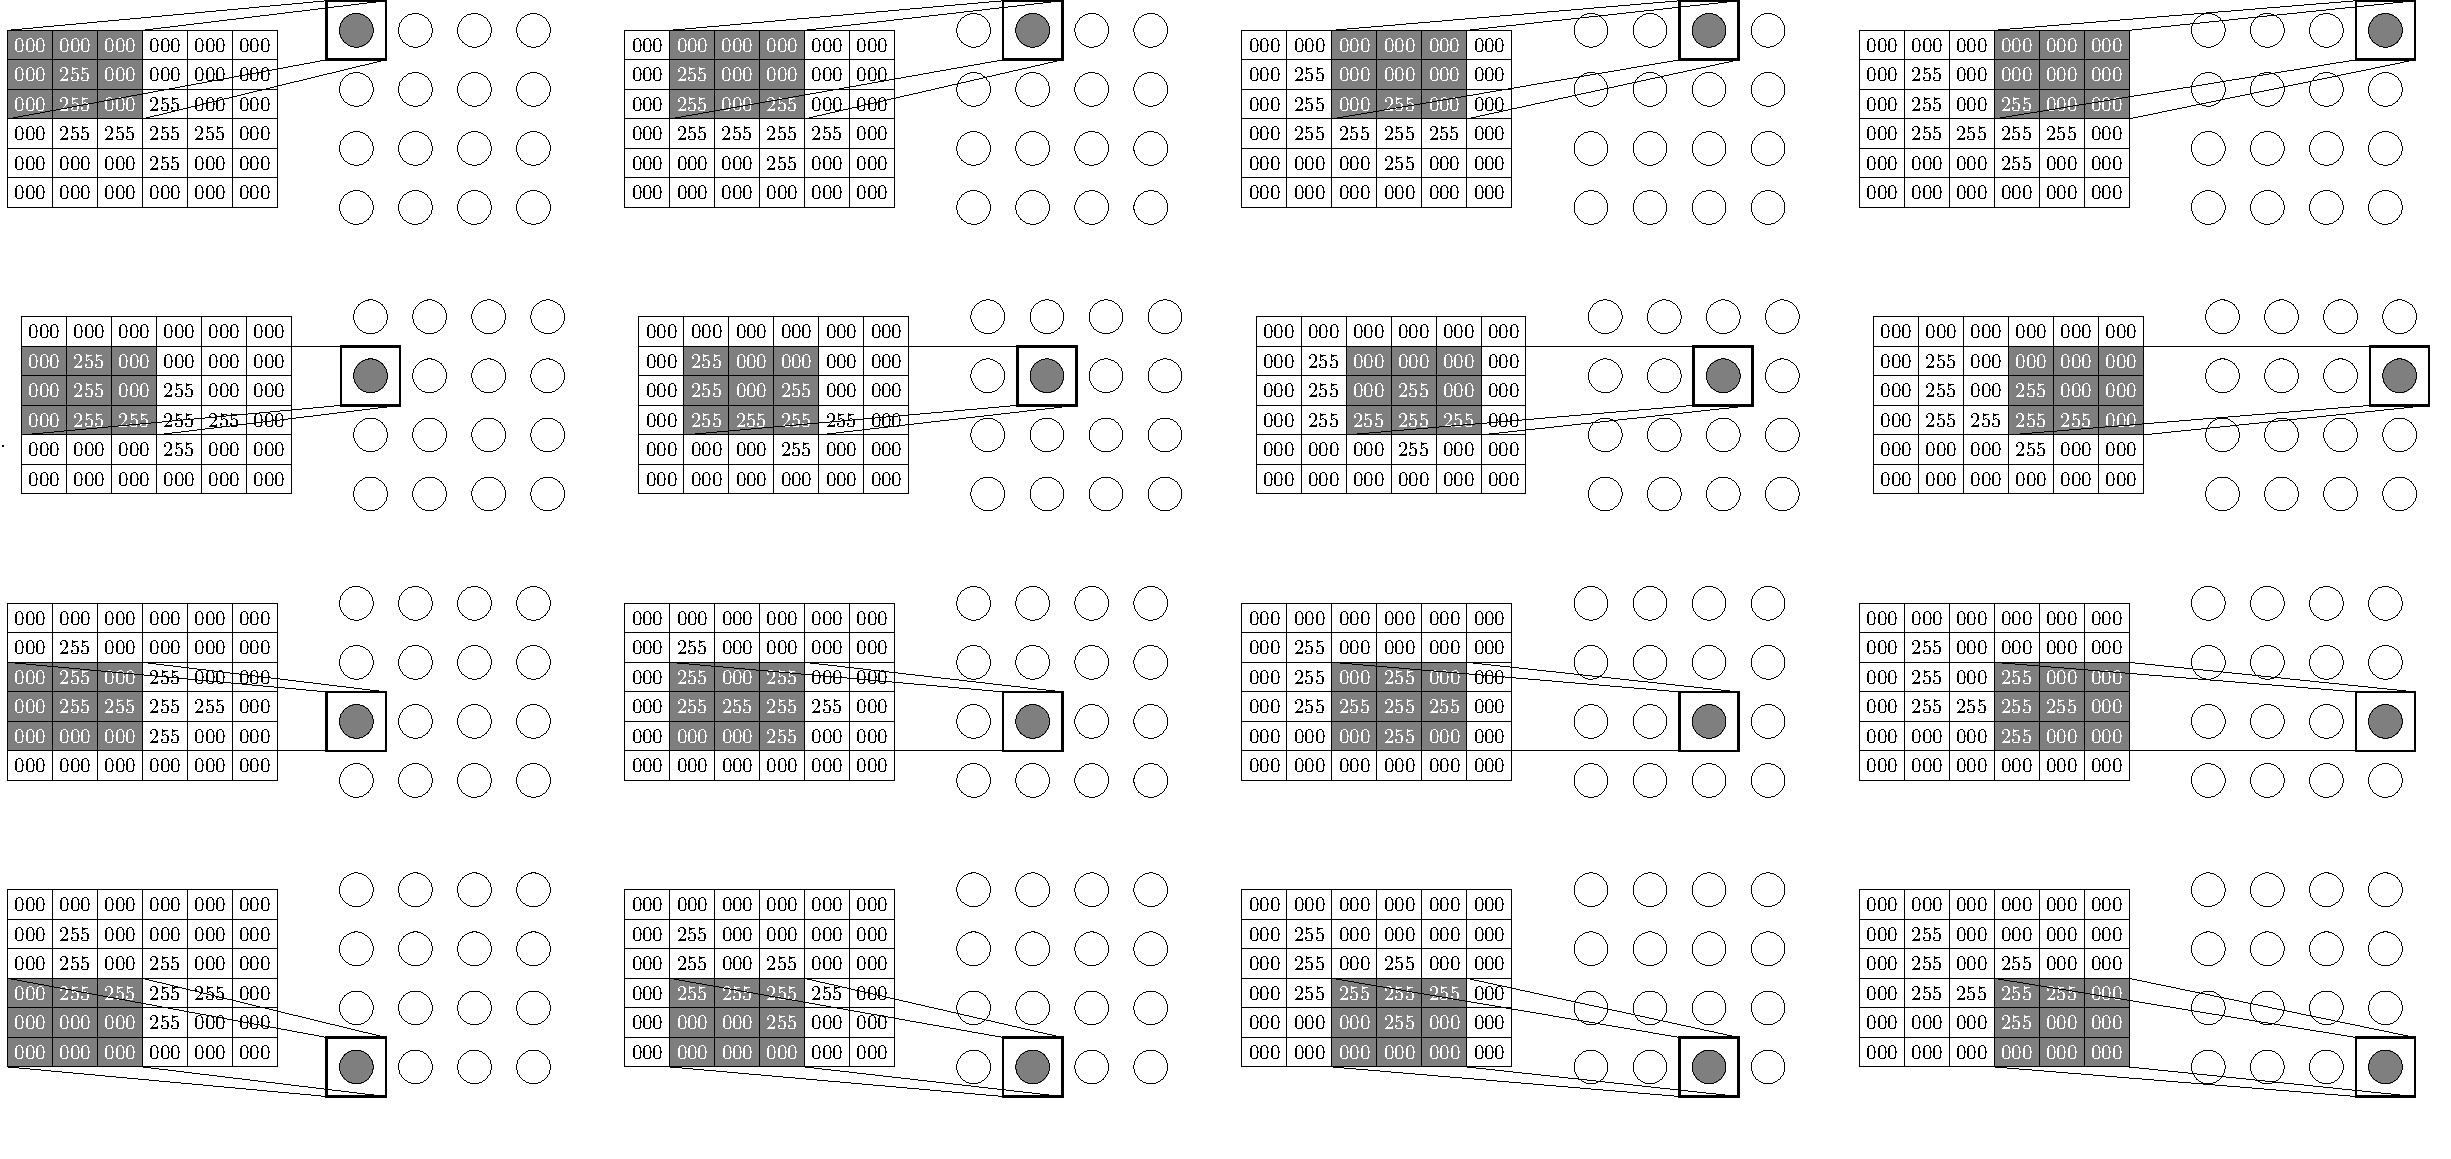
\includegraphics[width=\textwidth]{./images/fmlpda_8_33.pdf}
\caption{Illustration of the organization of a set of neurons that share weights (use the same filter) and their local receptive fields such that together the receptive fields cover the entirety of the input image.}
\label{fig:receptivefieldsorganization}
\end{figure}
\end{frame} 



 \begin{frame} 
\begin{alignat}{2}
\underbrace{
\footnotesize
\begin{bmatrix}
000 & 000 & 000 & 000 & 000 & 000\\
000 & \mathbf{255} & 000 & 000 & 000 & 000\\
000 & \mathbf{255} & 000 & \mathbf{255} & 000 & 000\\
000 & \mathbf{255} & \mathbf{255} & \mathbf{255} & \mathbf{255} & 000\\
000 & 000 & 000 & \mathbf{255} & 000 & 000\\
000 & 000 & 000 & 000 & 000 & 000\\
\end{bmatrix}
}_{\text{Input Image}}
&\rightarrow
\underbrace{
\footnotesize
\begin{bmatrix}
-1 & +1 & -1\\
-1 & +1 & -1\\
-1 & +1 & -1\\
\end{bmatrix}
}_{\text{Convolved Filter}}
&\rightarrow
\underbrace{
\footnotesize
\begin{bmatrix}
510 & 0 & 255 & 0\\
510 & 0 & 0 & 0\\
255 & 0 & 255 & 0\\
0 & 0 & 0 & 0\\
\end{bmatrix}
}_{\text{Feature Map}}
\label{eq:featuremap1}
\end{alignat}
\end{frame} 



 \begin{frame} 
\begin{alignat}{2}
\underbrace{
\footnotesize
\begin{bmatrix}
000 & 000 & 000 & 000 & 000 & 000\\
000 & \mathbf{255} & 000 & 000 & 000 & 000\\
000 & \mathbf{255} & 000 & \mathbf{255} & 000 & 000\\
000 & \mathbf{255} & \mathbf{255} & \mathbf{255} & \mathbf{255} & 000\\
000 & 000 & 000 & \mathbf{255} & 000 & 000\\
000 & 000 & 000 & 000 & 000 & 000\\
\end{bmatrix}
}_{\text{Input Image}}
&\rightarrow
\underbrace{
\footnotesize
\begin{bmatrix}
-1 & -1 & -1\\
+1 & +1 & +1\\
-1 & -1 & -1\\
\end{bmatrix}
}_{\text{Convolved Filter}}
&\rightarrow
\underbrace{
\footnotesize
\begin{bmatrix}
0 & 0 & 0 & 0\\
0 & 0 & 0 & 0\\
255 & 0 & 255 & 0\\
0 & 0 & 0 & 0\\
\end{bmatrix}
}_{\text{Feature Map}}
\label{eq:featuremap2}
\end{alignat}
\end{frame} 

\subsubsection{Filter hyper-parameters: Dimensions, stride and padding}


 \begin{frame} 
\begin{figure}[t]
\centerline{
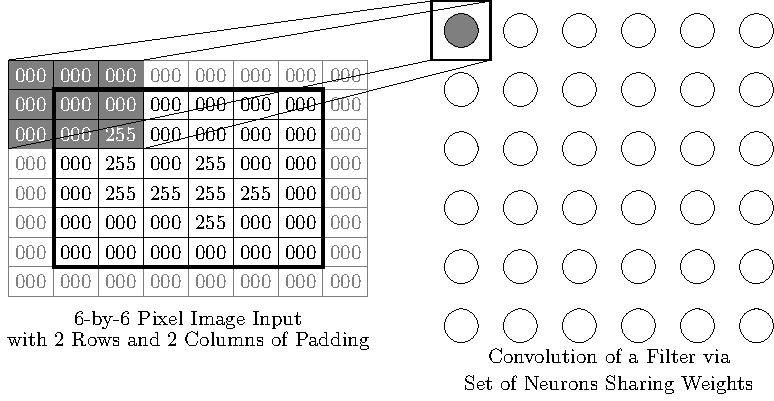
\includegraphics[width=\textwidth]{./images/fmlpda_8_34.pdf}
}
\caption{A grayscale image of a 4 after padding has been applied to the original 6-by-6 matrix representation, and the local receptive field of a neuron that includes both valid and padded pixels.}
\label{fig:cnn-padding}
\end{figure}
\end{frame} 


 \begin{frame} 
\noindent\scalebox{0.65}{\parbox{\linewidth}{%
\begin{alignat}{2}
\underbrace{
\begin{bmatrix}
000 & 000 & 000 & 000 & 000 & 000 & 000 & 000\\
000 & 000 & 000 & 000 & 000 & 000 & 000 & 000\\
000 & 000 & \mathbf{255} & 000 & 000 & 000 & 000& 000\\
000 & 000 & \mathbf{255} & 000 & \mathbf{255} & 000 & 000& 000\\
000 & 000 & \mathbf{255} & \mathbf{255} & \mathbf{255} & \mathbf{255} & 000& 000\\
000 & 000 & 000 & 000 & \mathbf{255} & 000 & 000& 000\\
000 & 000 & 000 & 000 & 000 & 000 & 000& 000\\
000 & 000 & 000 & 000 & 000 & 000 & 000 & 000\\
\end{bmatrix}
}_{\text{Input Image}}
&\rightarrow
\underbrace{
\begin{bmatrix}
-1 & +1 & -1\\
-1 & +1 & -1\\
-1 & +1 & -1\\
\end{bmatrix}
}_{\text{Convolved Filter}}
&\rightarrow
\underbrace{
\begin{bmatrix}
0 & 255 & 0 & 0 & 0 & 0\\
0 & 510 & 0 & 255 & 0 & 0\\
0 & 510 & 0 & 0 & 0 & 0\\
0 & 255 & 0 & 255 & 0 & 0\\
0 & 0 & 0 & 0 & 0 & 0\\
0 & 0 & 0 & 255 & 0 & 0\\
\end{bmatrix}
}_{\text{Feature Map}}
\label{eq:featuremap3}
\end{alignat}
}}
\end{frame} 



 \begin{frame} 
 \noindent\scalebox{0.65}{\parbox{\linewidth}{%
\begin{alignat}{3}
\underbrace{
\begin{bmatrix}
000 & 000 & 000 & 000 & 000 & 000 & 000 & 000\\
000 & 000 & 000 & 000 & 000 & 000 & 000 & 000\\
000 & 000 & \mathbf{255} & 000 & 000 & 000 & 000& 000\\
000 & 000 & \mathbf{255} & 000 & \mathbf{255} & 000 & 000& 000\\
000 & 000 & \mathbf{255} & \mathbf{255} & \mathbf{255} & \mathbf{255} & 000& 000\\
000 & 000 & 000 & 000 & \mathbf{255} & 000 & 000& 000\\
000 & 000 & 000 & 000 & 000 & 000 & 000& 000\\
000 & 000 & 000 & 000 & 000 & 000 & 000 & 000\\
\end{bmatrix}
}_{\text{Input Image}}
&\rightarrow
\underbrace{
\begin{bmatrix}
-1 & -1 & -1\\
+1 & +1 & +1\\
-1 & -1 & -1\\
\end{bmatrix}
}_{\text{Convolved Filter}}
&\rightarrow
\underbrace{
\begin{bmatrix}
0 & 0 & 0 & 0 & 0 & 0\\
0 & 0 & 0 & 0 & 0 & 0\\
0 & 0 & 0 & 0 & 0 & 0\\
0 & 255 & 0 & 255 & 0 & 255\\
0 & 0 & 0 & 0 & 0 & 0\\
0 & 0 & 0 & 0 & 0 & 0\\
\end{bmatrix}
}_{\text{Feature Map}}
\label{eq:featuremap4}
\end{alignat}
}}
\end{frame} 

\subsubsection{Pooling}

 \begin{frame} 
 \noindent\scalebox{0.65}{\parbox{\linewidth}{%
\begin{alignat}{2}
\underbrace{
\begin{bmatrix}
000 & 000 & 000 & 000 & 000 & 000 & 000 & 000\\
000 & 000 & 000 & 000 & 000 & 000 & 000 & 000\\
000 & 000 & \mathbf{255} & 000 & 000 & 000 & 000& 000\\
000 & 000 & \mathbf{255} & 000 & \mathbf{255} & 000 & 000& 000\\
000 & 000 & \mathbf{255} & \mathbf{255} & \mathbf{255} & \mathbf{255} & 000& 000\\
000 & 000 & 000 & 000 & \mathbf{255} & 000 & 000& 000\\
000 & 000 & 000 & 000 & 000 & 000 & 000& 000\\
000 & 000 & 000 & 000 & 000 & 000 & 000 & 000\\
\end{bmatrix}
}_{\text{Input Image}}
&\rightarrow
\underbrace{
\begin{bmatrix}
-1 & -1 & -1\\
+1 & +1 & +1\\
-1 & -1 & -1\\
\end{bmatrix}
}_{\text{Convolved Filter}}
\rightarrow \notag \\
\rightarrow
\underbrace{
\begin{bmatrix}
0 & 0 & 0 & 0 & 0 & 0\\
0 & 0 & 0 & 0 & 0 & 0\\
0 & 0 & 0 & 0 & 0 & 0\\
0 & 255 & 0 & 255 & 0 & 255\\
0 & 0 & 0 & 0 & 0 & 0\\
0 & 0 & 0 & 0 & 0 & 0\\
\end{bmatrix}
}_{\text{Feature Map}}
&\rightarrow \text{max pooling} \rightarrow
\underbrace{
\begin{bmatrix}
0 & 0 & 0\\
255 & 255 & 255\\
0 & 0 & 0\\
\end{bmatrix}
}_{\text{Output from Sub-sampling}}
\label{eq:poolingexample}
\end{alignat}
}}
\end{frame} 



 \begin{frame} 
\begin{alignat}{2}
\underbrace{
\begin{bmatrix}
\text{O} & \text{O} & \text{O} & \text{O} & \text{O} & \text{O} \\
\text{O} & \text{O} & \text{O} & \text{O} & \text{O} & \text{O} \\
\text{A} & \text{O} & \text{O} & \text{O} & \text{O} & \text{O} \\
\text{O} & \text{B} & \text{O} & \text{O} & \text{O} & \text{O} \\
\text{O} & \text{O} & \text{O} & \text{O} & \text{O} & \text{O} \\
\text{O} & \text{O} & \text{O} & \text{O} & \text{O} & \text{O} \\
\end{bmatrix}
}_{\text{Neurons that convolve the Filter}}
&\rightarrow 
\underbrace{
\begin{bmatrix}
\text{O} & \text{O} & \text{O}\\
\text{C} & \text{O} & \text{O}\\
\text{O} & \text{O} & \text{O}\\
\end{bmatrix}
}_{\text{Sub-sampling Layer}}
&\rightarrow 
\underbrace{
\begin{bmatrix}
\text{D}\\
\text{E}\\
\end{bmatrix}
}_{\text{Fully Connected Layer}}
\label{eq:cnn-backprop-example} 
\end{alignat}
\end{frame} 



 \begin{frame} 
\begin{alignat}{2}
\delta_C &= \hspace{1.8cm}\frac{\partial \mathcal{E}}{\partial a_C} &\times &\frac{\partial a_C}{ \partial z_C} \notag\\ 
~ &= \left( \left( \delta_D \times w_{D,C} \right) + \left( \delta_E \times w_{E,C} \right) \right) & \times & \phantom{O}1 \notag\\
\label{eqn:neuronCdelta}
\end{alignat}
\end{frame} 



 \begin{frame} 
\begin{alignat}{2}
\delta_B &= \hspace{0.45cm}\frac{\partial \mathcal{E}}{\partial a_B} &\times &\frac{\partial a_B}{ \partial z_B} \notag\\ 
~ &= \left( \delta_D \times w_{C,B} \right) & \times & \frac{\partial a_B}{ \partial z_B} \notag\\
~ &= \left( \delta_D \times 1 \right) & \times & \phantom{O}1 \notag\\
\label{eqn:neuronBdelta}
\end{alignat}
\end{frame} 

\subsubsection{Handling color images and multiple filters}

 \begin{frame} 
 \begin{alignat}{2}
    \left[
  \underbrace{w_0}_{\text{bias}}
  \left[ {\begin{array}{cc}
   w_1 & w_2 \\
   w_3 & w_4 \\
  \end{array} } \right]
    \left[ {\begin{array}{cc}
   w_5 & w_6 \\
   w_7 & w_8 \\
  \end{array} } \right]
    \left[ {\begin{array}{cc}
   w_9 & w_{10} \\
   w_{11} & w_{12} \\
  \end{array} } \right]
  \right]
  \label{eqn:threedimensionalfilter}
\end{alignat}
\end{frame} 



 \begin{frame} 
 \noindent\scalebox{0.9}{\parbox{\linewidth}{%
 \begin{alignat}{2}
    \left[
  \underbrace{w_0=0.5}_{\text{bias}}
    \underbrace{
  \left[ {\begin{array}{cc}
   w_1=1 & w_2=1 \\
   w_3=0 & w_4=0 \\
  \end{array} } \right]
  }_{\text{Red Channel}}
  \underbrace{
    \left[ {\begin{array}{cc}
   w_5=0 & w_6=1 \\
   w_7=0 & w_8=1 \\
  \end{array} } \right]
  }_{\text{Green Channel}}
  \underbrace{
    \left[ {\begin{array}{cc}
   w_9=1 & w_{10}=0 \\
   w_{11}=0 & w_{12}=1 \\
  \end{array} } \right]
  }_{\text{Blue Channel}}
  \right]
  \label{eqn:3dfilterannotated}
\end{alignat}
}}
\end{frame} 



 \begin{frame} 
 \begin{equation}
    \left[
    \underbrace{
  \left[ {\begin{array}{ccc}
   1 & 1 & 1 \\
   0 & 0 & 0 \\
   0 & 0 & 0 \\ 
  \end{array} } \right]
  }_{\text{Red Channel}}
  \underbrace{
    \left[ {\begin{array}{ccc}
   0 & 0 & 2 \\
   0 & 0 & 2 \\
   0 & 0 & 2 \\
  \end{array} } \right]
  }_{\text{Green Channel}}
  \underbrace{
    \left[ {\begin{array}{ccc}
   3 & 0 & 0 \\
   0 & 3 & 0 \\
   0 & 0 & 3 \\
  \end{array} } \right]
  }_{\text{Blue Channel}}
  \right]
  \label{eqn:3dimage}
\end{equation}
\end{frame} 



 \begin{frame} 
 \begin{equation}
    \left[
    \underbrace{
  \left[ {\begin{array}{ccc}
   1 & 1 \\
   0 & 0 \\
  \end{array} } \right]
  }_{\text{Red Channel}}
  \underbrace{
    \left[ {\begin{array}{ccc}
   0 & 0 \\
   0 & 0 \\
  \end{array} } \right]
  }_{\text{Green Channel}}
  \underbrace{
    \left[ {\begin{array}{ccc}
   3 & 0 \\
   0 & 3 \\
  \end{array} } \right]
  }_{\text{Blue Channel}}
  \right]
  \label{eqn:3dlocalreceptivefield}
\end{equation}
\end{frame} 



 \begin{frame} 
 \begin{alignat}{2}
z&= ( ( w_0 \times 1)\notag\\
   &\hspace{0.5cm}+ (w_1 \times 1) + (w_2 \times 1) + (w_3 \times 0) + (w_4\times0) \notag \\
   &\hspace{0.5cm}+ ( w_5 \times 0) + (w_6 \times 0) + (w_7 \times 0) + (w_8 \times 0) \notag\\
   &\hspace{0.5cm}+ ( w_9 \times 3) + (w_{10} \times 0) + (w_{11} \times 0) + (w_{12} \times 3)) \notag\\ 
   &= 0.5 + 1 + 1 + 0 + 0 + 0 + 0 + 0 + 0 + 3 + 0 + 0 + 3 \notag\\
   &= 8.5\notag\\
 a&=rectifier(z)\notag\\
 &=rectifier(8.5)\notag\\
   &=8.5
   \label{eqn:relufilteractivationcalc}
\end{alignat}
\end{frame} 



 \begin{frame} 
 \begin{equation}
    \left[ {\begin{array}{ccc}
   8.5 & 6.5 \\
   0.5 & 10.5 \\
  \end{array} } \right]
  \label{eqn:2dfeaturemap}
\end{equation}
\end{frame} 



 \begin{frame}[plain]
\begin{figure}[!b]
\centerline{
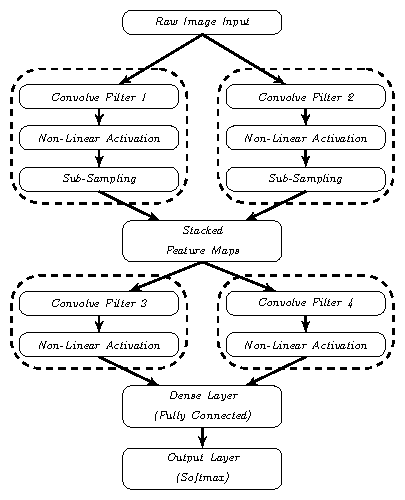
\includegraphics[width=0.6\textwidth]{./images/fmlpda_8_35.pdf}
}
\caption{Schematic of the typical sequences of layers found in a convolutional neural network.}
\label{fig:cnn-architecture}
\end{figure}
\end{frame} 



 \begin{frame} 
\begin{figure}
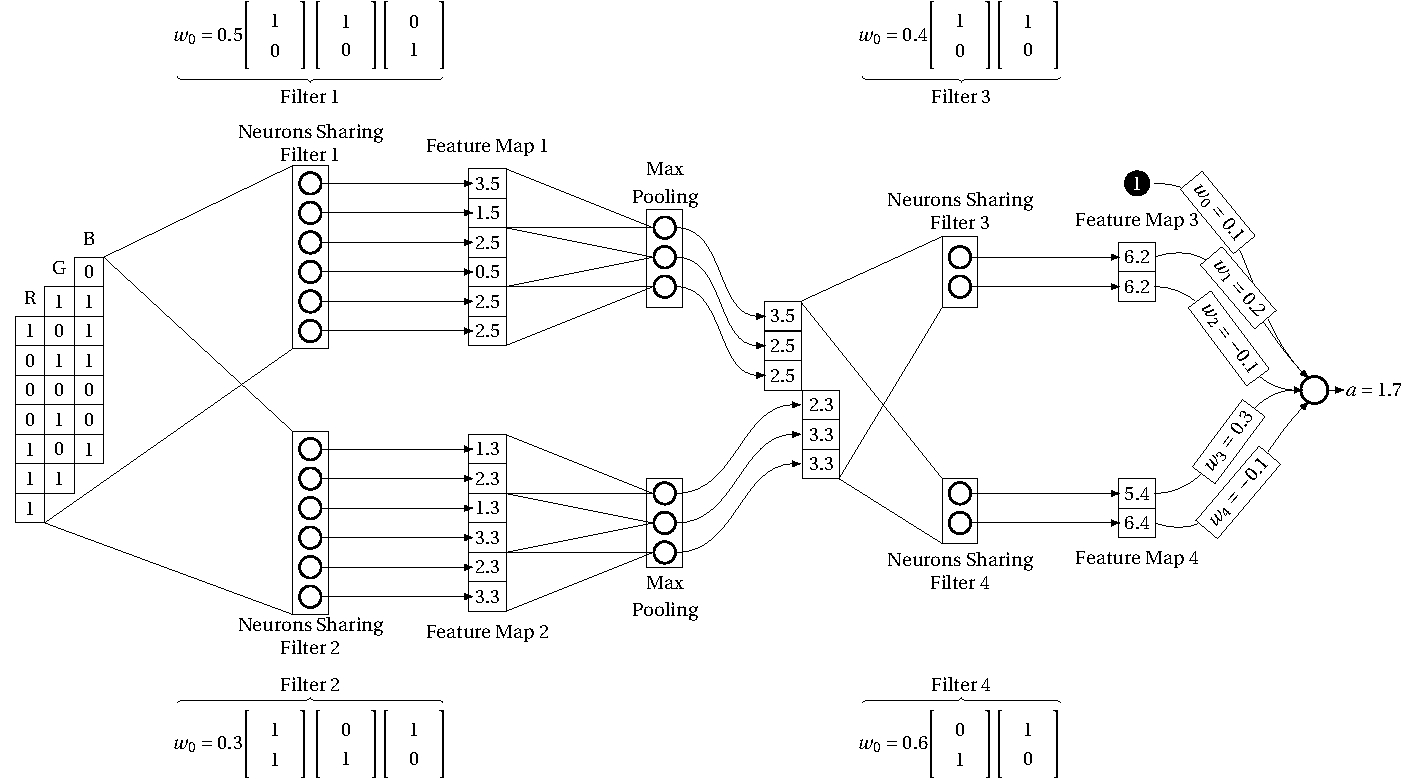
\includegraphics[width=\textwidth]{./images/fmlpda_8_36.pdf}
\caption{Worked example illustrating the dataflow through a multilayer, multifilter CNN.}
\label{fig:cnn-multilayer-multifilter}
\end{figure}
\end{frame} 


\subsection{Sequential Models: Recurrent Neural Networks and Long Short-Term Memory Networks}

\subsubsection{Simple recurrent neural networks}

 \begin{frame} 
\begin{figure}[t]
\centerline{
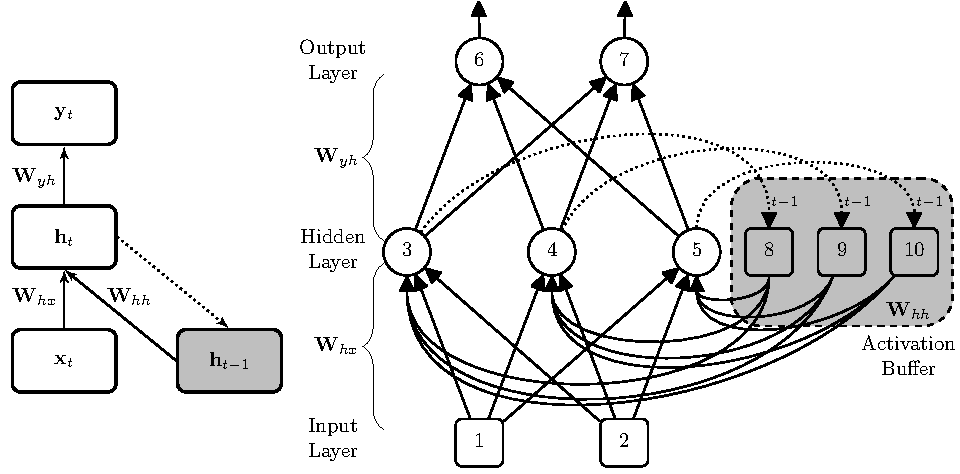
\includegraphics[width=\textwidth]{./images/fmlpda_8_37.pdf}
}
\caption[Schematic of the simple recurrent neural architecture.]{Schematic of the simple recurrent neural architecture.}
\label{fig:rnn-architecture}
\end{figure}
\end{frame} 

 \begin{frame} 
\begin{alignat}{1}
\mathbf{h}_t &= \varphi\left(\left(\mathbf{W}_{hh} \cdot \mathbf{h}_{t-1}\right) + \left(\mathbf{W}_{hx} \cdot \mathbf{x}_t \right) + \mathbf{w}_0\right) \label{eq:rnnhidden}\\
\mathbf{y}_t &= \varphi\left(\mathbf{W}_{yh} \cdot \mathbf{h}_t \right) \label{eq:rnnoutput}
\end{alignat}
\end{frame} 

\subsubsection{Backpropagation through time}

 \begin{frame} 
\begin{figure}[t]
\centerline{
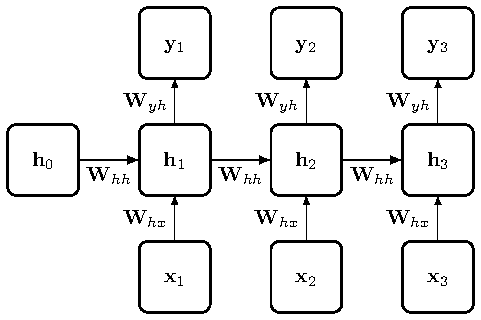
\includegraphics[width=0.8\textwidth]{./images/fmlpda_8_38.pdf}
}
\caption[A simple RNN model unrolled through time (in this instance, three time-steps).]{A simple RNN model unrolled through time (in this instance, three time-steps).}
\label{fig:rnn-unrolledthroughtime}
\end{figure}
\end{frame} 



 \begin{frame}[plain]
\begin{figure}[t]
\centerline{
\includegraphics[width=0.3\textwidth]{./images/fmlpda_8_39.pdf}
}
\caption{An illustration of the different iterations of backpropagation during backpropagation through time.}
\label{fig:bptt}
\end{figure}
\end{frame} 


\begin{frame}[plain]
\begin{algorithm}[H]
\tiny
\caption[The Backpropagation Through Time Algorithm]{The Backpropagation Through Time Algorithm}
\begin{algorithmic}[1]
\Require $h_0$ initialized hidden state
\Require $\mathbf{x}$ a sequence of inputs
\Require $\mathbf{y}$ a sequence of target outputs 
\Require $n$ length of the input sequence
\Require Initialized weight matrices (with associated biases)
\Require $\Delta \mathbf{w}$ a data structure to accumulate the summed weight updates for each weight across time-steps
\For{$t=1$ to $n$}
	\State $Inputs = \lbrack x_0, \dots, x_t \rbrack$
	\State $h_{tmp} = h_0$
	\For{$i=0$ to $t$} 
	\Comment Unroll the network through $t$ steps
		\State $h_{tmp} = ForwardPropagate(Inputs\lbrack i \rbrack,h_{tmp})$
	\EndFor
	\State $\hat{y}_t = OutputLayer(h_{tmp})$
	\Comment Generate the output for time-step $t$
	\State $\mathcal{E}_t = \mathbf{y}\lbrack t\rbrack - \hat{y}_t$
	\Comment Calculate the error at time-step $t$
	\State $Backpropagate(\mathcal{E}_t)$ 
	\Comment{Backpropagate $\mathcal{E}_t$ through $t$ steps}
	\State For each weight, sum the weight updates across the unrolled network and update $\Delta \mathbf{w}$	
\EndFor
\State Update the network weights using $\Delta \mathbf{w}$
\end{algorithmic}
\label{alg:bptt}
\end{algorithm}
\end{frame}



\subsubsection{Long short-term memory networks}


 \begin{frame} 
\begin{figure}[t]
\centerline{
\includegraphics[width=\textwidth]{./images/fmlpda_8_40.pdf}
}
\caption{A schematic of the internal structure of a long short-term memory unit. This figure is based on Figure 5.4 of \citep{kelleher:2019}, which in turn was inspired by an image by Christopher Olah (available at: \url{http://colah.github.io/posts/2015-08-Understanding-LSTMs/}).}
\label{fig:lstm}
\end{figure}
\end{frame} 



 \begin{frame} 
\begin{alignat}{2}
\mathbf{f}_t &= \varphi_{sigmoid}(\mathbf{W}^{(f)} \cdot \mathbf{hx}_t) \label{eqn:forgetmask}\\
\mathbf{c\ddagger} &= \mathbf{c}_{t-1} \odot \mathbf{f}_t \label{eqn:forgetcellupdated}\\
\notag
\end{alignat}
\end{frame} 



 \begin{frame} 
\begin{alignat}{2}
 \mathbf{c}_{t-1} &= 
 \left[
  \begin{array}{c}
1 \\
1 \\
1\\
  \end{array} 
  \right] 
 \mathbf{h}_{t-1} = 
 \left[
 \begin{array}{c}
   1 \\
   1 \\
  \end{array} 
  \right] 
 \mathbf{x}_{t}  = 
 \left[
 \begin{array}{c}
   4 \\
  \end{array} 
  \right] \notag\\
  \mathbf{W}^{(f)} & = 
 \left[
 \begin{array}{cccc}
 0 & \phantom{-}1 & \phantom{-}1 & \phantom{-}1\\
 0 & -1 & -1 & -1\\
 0 & \phantom{-}0 & \phantom{-}0 & \phantom{-}0\\
 \end{array}
 \right]\notag \\
\label{eqn:lstmforgetgatestate}
\end{alignat}
\end{frame} 



 \begin{frame} 
 \noindent\scalebox{0.9}{\parbox{\linewidth}{%
\begin{alignat}{2}
 ~&
 \underbrace{
 \left[
 \begin{array}{cccc}
 0 & \phantom{-}1 & \phantom{-}1 & \phantom{-}1\\
 0 & -1 & -1 & -1\\
 0 & \phantom{-}0 & \phantom{-}0 & \phantom{-}0\\
 \end{array}
 \right]
 }_{\mathbf{W}^{(f)}}
 \times  
 \underbrace{
 \left[
 \begin{array}{c}
   1\\
   1 \\
   1 \\
   4\\
  \end{array} 
 \right]
 }_{\mathbf{hx}_t}
 =
 \underbrace{
 \left[
 \begin{array}{c}
   \phantom{-}6\\
   -6 \\
   \phantom{-}0 \\
  \end{array} 
 \right]
 }_{\mathbf{Z}_{t}^{(f)}}
\rightarrow
\varphi_{sigmoid}
\rightarrow
\underbrace{
 \left[
 \begin{array}{c}
0.997527377\\
0.002472623\\
0.500000000\\
  \end{array} 
 \right]
 }_{\mathbf{f}_t}\notag\\
~&\underbrace{
 \left[
 \begin{array}{c}
0.997527377\\
0.002472623\\
0.500000000\\
  \end{array} 
 \right]
 }_{\mathbf{f}_t}
\odot
\underbrace{
 \left[
 \begin{array}{c}
1\\
1 \\
1 \\
  \end{array} 
 \right]
 }_{\mathbf{c}_{t-1}}
=
\underbrace{
 \left[
 \begin{array}{c}
0.997527377\\
0.002472623\\
0.500000000\\
  \end{array} 
 \right]
}_{\mathbf{c\ddagger}} 
 \notag\\
\end{alignat}
}}
\end{frame} 



 \begin{frame} 
\begin{alignat}{2}
\mathbf{i\dagger}_t &= \varphi_{sigmoid}(\mathbf{W}^{(i\dagger)} \cdot \mathbf{hx}_t) \label{eqn:inputmask}\\
\mathbf{i\ddagger}_t &= \varphi_{tanh}(\mathbf{W}^{(i\ddagger)} \cdot \mathbf{hx}_t) \label{eqn:inputupdate}\\
\mathbf{i}_t & = \mathbf{i\dagger}_t \odot \mathbf{i\ddagger}_t \label{eqn:input}\\
\mathbf{c}_t & = \mathbf{c\ddagger} + \mathbf{i}_t \label{eqn:inputcellupdate}
\end{alignat}
\end{frame} 



 \begin{frame} 
\begin{alignat}{2}
\mathbf{o\dagger}_t &= \varphi_{sigmoid}(\mathbf{W}^{(o\dagger)} \cdot \mathbf{hx}_t) \label{eqn:outputmask}\\
\mathbf{o\ddagger}_t &= \varphi_{tanh}(\mathbf{W}^{(o\ddagger)} \cdot \mathbf{c}_t) \label{eqn:candidateoutput}\\
\mathbf{o}_t &= \mathbf{o\dagger}_t \odot \mathbf{o\ddagger}_t \label{eqn:outputstate}\\
\mathbf{h}_{t+1} & = \mathbf{o}_t  \label{eqn:hpropogated}
\end{alignat}
\end{frame} 



 \begin{frame} 
\begin{alignat}{2}
\mathbf{f}_t &= \varphi_{sigmoid}(\mathbf{W}^{(f)} \cdot \mathbf{hx}_t) \notag\\
\mathbf{c\ddagger} &= \mathbf{c}_{t-1} \odot \mathbf{f}_t \notag\\
\mathbf{i\dagger}_t &= \varphi_{sigmoid}(\mathbf{W}^{(i\dagger)} \cdot \mathbf{hx}_t) \notag\\
\mathbf{i\ddagger}_t &= \varphi_{tanh}(\mathbf{W}^{(i\ddagger)} \cdot \mathbf{hx}_t) \notag\\
\mathbf{i}_t & = \mathbf{i\dagger}_t \odot \mathbf{i\ddagger}_t \notag\\
\mathbf{c}_t & = \mathbf{c\ddagger} + \mathbf{i}_t\notag\\
\mathbf{o\dagger}_t &= \varphi_{sigmoid}(\mathbf{W}^{(o\dagger)} \cdot \mathbf{hx}_t)\notag\\
\mathbf{o\ddagger}_t &= \varphi_{tanh}(\mathbf{W}^{(o\ddagger)} \cdot \mathbf{c}_t) \notag\\
\mathbf{o}_t &= \mathbf{o\dagger}_t \odot \mathbf{o\ddagger}_t \notag\\
\mathbf{h}_{t+1} & = \mathbf{o}_t \notag
\end{alignat}
\end{frame} 



 \begin{frame} 
\begin{figure}[t]
\centerline{
\includegraphics[width=0.75\textwidth]{./images/fmlpda_8_41.pdf}
}
\caption{The flow of activations through a long short-term memory unit during forward propagation when $\mathbf{c}_{t{-}1}=\lbrack 0.3, 0.6\rbrack$, $\mathbf{h}_{t}=\lbrack 0.1, 0.8\rbrack$, and $\mathbf{x}_{t}=\lbrack 0.9 \rbrack$.}
\label{fig:lstm-forwardprop}
\end{figure}
\end{frame} 

\subsubsection{Backpropagating through an LSTM cell}

 \begin{frame} 
\begin{figure}[t]
\centerline{
\includegraphics[width=\textwidth]{./images/fmlpda_8_42.pdf}
}
\caption[The flow of error gradients through a long short-term memory unit during backpropagation.]{The flow of error gradients through a long short-term memory unit during backpropagation.}
\label{fig:lstm-backprop}
\end{figure}
\end{frame} 



 \begin{frame} 
\begin{equation}
\frac{\partial \mathcal{E}}{\partial \mathbf{o}_t} = \frac{\partial \mathcal{E}_t}{\partial \mathbf{o}_t}  + \frac{\partial \mathcal{E}_{t{+}1}}{\partial \mathbf{h}_{t}}
\label{eqn:lstmoutputerrgrad}
\end{equation}
\end{frame} 



 \begin{frame} 
\begin{alignat}{2}
\frac{\partial \mathcal{E}}{\partial \mathbf{o\ddagger}} & = \frac{\partial \mathcal{E}}{\partial \mathbf{o}_t} \odot \mathbf{o\dagger} \label{eqn:outputdoubledaggergradient}\\
\frac{\partial \mathcal{E}}{\partial \mathbf{o\dagger}} & = \frac{\partial \mathcal{E}}{\partial \mathbf{o}_t} \odot \mathbf{o\ddagger} \label{eqn:outputdaggergradient}
\end{alignat}
\end{frame} 



 \begin{frame} 
\begin{alignat}{2}
	\mathbf{\delta}_{o\ddagger} & = \frac{\partial \mathcal{E}}{\partial \mathbf{o\ddagger}} \odot \frac{\partial \mathbf{o\ddagger}_t}{\partial \mathbf{c}_{t\ddagger}}  &= & \frac{\partial \mathcal{E}}{\partial \mathbf{o\ddagger}} \odot \underbrace{\left(\mathbf{1} - tanh^2(\mathbf{c\ddagger}_t) \right)}_{\text{Derivate of tanh, i.e.:}\frac{\partial a}{\partial z}}	\label{eqn:outputTdelta}\\ 
\frac{\partial \mathcal{E}}{\partial \mathbf{c}_t} & = \mathbf{\delta}_{o\ddagger}+ \frac{\partial \mathcal{E}_{t{+}1}}{\partial \mathbf{c}_t} \label{eqn:mergeoutputerrandcellerr}
\end{alignat}
\end{frame} 



 \begin{frame} 
\begin{alignat}{2}
\frac{\partial \mathcal{E}}{\partial \mathbf{i\ddagger}} & = \frac{\partial \mathcal{E}}{\partial \mathbf{c}_t} \odot \mathbf{i\dagger} \label{eqn:inputdoubledaggergradient}\\
\frac{\partial \mathcal{E}}{\partial \mathbf{i\dagger}} & = \frac{\partial \mathcal{E}}{\partial \mathbf{c}_t} \odot \mathbf{i\ddagger} \label{eqn:inputdaggergradient}
\end{alignat}
\end{frame} 



 \begin{frame} 
\begin{alignat}{2}
\frac{\partial \mathcal{E}}{\partial \mathbf{c}_{t-1}} & = \frac{\partial \mathcal{E}}{\partial \mathbf{c}_t} \odot \mathbf{f}_t \label{eqn:gradientcellold}\\
\frac{\partial \mathcal{E}}{\partial \mathbf{f}} & = \frac{\partial \mathcal{E}}{\partial \mathbf{c}_t} \odot \mathbf{c}_{t{-}1} \label{eqn:gradientforgetmask}
\end{alignat}
\end{frame} 



 \begin{frame} 
\begin{alignat}{4}
	\mathbf{\delta}_f & = \frac{\partial \mathcal{E}}{\partial \mathbf{f}} \odot \frac{\partial \mathbf{f}_t}{\partial \mathbf{z}_f}  &= &\frac{\partial \mathcal{E}}{\partial \mathbf{f}} \odot \left( \mathbf{f}_t \odot \left(\mathbf{1} - \mathbf{f}_t\right)  \right) \label{eqn:forgetdelta}\\
	\mathbf{\delta}_{i\dagger} & = \frac{\partial \mathcal{E}}{\partial \mathbf{i\dagger}} \odot \frac{\partial \mathbf{i\dagger}_t}{\partial \mathbf{z}_{i\dagger}}  &= & \frac{\partial \mathcal{E}}{\partial \mathbf{i\dagger}} \odot \left( \mathbf{i\dagger}_t \odot \left(\mathbf{1} - \mathbf{i\dagger}_t\right)  \right) \label{eqn:idaggerdelta}\\
	\mathbf{\delta}_{i\ddagger} & = \frac{\partial \mathcal{E}}{\partial \mathbf{i\ddagger}} \odot \frac{\partial \mathbf{i\ddagger}_t}{\partial \mathbf{z}_{i\ddagger}}  &= & \frac{\partial \mathcal{E}}{\partial \mathbf{i\ddagger}} \odot \left(\mathbf{1} - tanh^2(\mathbf{i\ddagger}_t)  \right) \label{eqn:idoubledaggerdelta}\\
	\mathbf{\delta}_{o\dagger} & = \frac{\partial \mathcal{E}}{\partial \mathbf{o\dagger}} \odot \frac{\partial \mathbf{o\dagger}_t}{\partial \mathbf{z}_{o\dagger}}  &= & \frac{\partial \mathcal{E}}{\partial \mathbf{o\dagger}} \odot \left( \mathbf{o\dagger}_t \odot \left(\mathbf{1} - \mathbf{o\dagger}_t\right)  \right) \label{eqn:odaggerdelta}\end{alignat}
\end{frame} 



 \begin{frame} 
\begin{equation}
\Delta \mathbf{W}^{(f)} = \mathbf{\delta}_f \cdot \mathbf{hx}^\intercal
\end{equation}
\end{frame} 



 \begin{frame} 
\begin{equation*}
\frac{\partial \mathcal{E}_{t{+}1}}{\partial \mathbf{c}_t}=\begin{bmatrix} 0.35 \\ 0.50 \end{bmatrix} \quad
\frac{\partial \mathcal{E}_{t{+}1}}{\partial \mathbf{h}_t}=\begin{bmatrix} 0.75 \\ 0.25\end{bmatrix} \quad
\frac{\partial \mathcal{E}_{t}}{\partial \mathbf{o}_t}=\begin{bmatrix} 0.15 \\ 0.60\end{bmatrix} \notag
\end{equation*}
\end{frame} 



 \begin{frame} 
\begin{alignat}{2}
	 \frac{\partial \mathcal{E}}{\partial \mathbf{o}_t}&=\underbrace{\begin{bmatrix} 0.75\\ 0.25\end{bmatrix}}_{\partial \mathcal{E}_{t{+}1}/\partial \mathbf{h}_t} + \underbrace{\begin{bmatrix} 0.15\\ 0.60 \end{bmatrix}}_{\partial \mathcal{E}_{t}/\partial \mathbf{o}_t}  = \begin{bmatrix} 0.9\\ 0.85 \end{bmatrix} \label{eqn:exampleeotgrad}\\
	 \frac{\partial \mathcal{E}}{\partial \mathbf{o\ddagger}}&= \underbrace{\begin{bmatrix} 0.9\\ 0.85 \end{bmatrix}}_{\partial \mathcal{E}/\partial \mathbf{o}_t} \odot \underbrace{\begin{bmatrix}  0.575420058\\ 0.52098661 \end{bmatrix}}_{\mathbf{o\dagger}}  = \begin{bmatrix}0.517878052\\ 0.442839512\end{bmatrix} \\
	 \delta_{o\ddagger}& = \underbrace{\begin{bmatrix}0.517878052\\ 0.442839512\end{bmatrix}}_{\partial \mathcal{E}/\partial \mathbf{o\ddagger}} \odot \underbrace{\begin{bmatrix} 0.999184559\\ 0.997048635 \end{bmatrix}}_{1-tanh(\mathbf{c}_t)} = \begin{bmatrix} 0.517455753\\ 0.441532531 \end{bmatrix}\\
	 \frac{\partial \mathcal{E}}{\partial \mathbf{c}_t} &= \underbrace{\begin{bmatrix} 0.517455753\\ 0.441532531 \end{bmatrix}}_{\delta_{o\ddagger}} + \underbrace{\begin{bmatrix} 0.35\\ 0.50\end{bmatrix}}_{\partial \mathcal{E}_{t{+}1}/\partial \mathbf{c}_t}  = \begin{bmatrix} 0.867455753\\ 0.941532531 \end{bmatrix} \label{eqn:gradECTexample}
\end{alignat}
\end{frame} 



 \begin{frame} 
\begin{alignat}{2}
	 \frac{\partial \mathcal{E}}{\partial \mathbf{f}} & = \underbrace{\begin{bmatrix} 0.867455753\\ 0.941532531 \end{bmatrix}}_{\partial \mathcal{E}/\partial \mathbf{c}_t} \odot \underbrace{\begin{bmatrix} 0.3\\ 0.6\end{bmatrix}}_{\mathbf{c}_{t{-}1}}  = \begin{bmatrix} 0.260236726\\ 0.564919518 \end{bmatrix}\\
	 \mathbf{\delta}_f & = \underbrace{\begin{bmatrix} 0.260236726\\ 0.564919518 \end{bmatrix}}_{\partial \mathcal{E}/\partial \mathbf{f}} \odot \underbrace{ \begin{bmatrix} 0.248743973\\ 0.249694 \end{bmatrix} }_{\mathbf{f}_t \odot (1-\mathbf{f}_t)} = \begin{bmatrix} 0.064732317\\ 0.141057014 \end{bmatrix}\\
	 \Delta \mathbf{W}^{(f)} & = \underbrace{\begin{bmatrix} 0.064732317\\ 0.141057014 \end{bmatrix}}_{\mathbf{\delta}_f} \cdot \underbrace{\begin{bmatrix} 1.00 & 0.10 & 0.80 & 0.90  \end{bmatrix}}_{\mathbf{hx}^\intercal} \notag\\
	 & = \begin{bmatrix} 
	 0.064732317& 	0.006473232 &	0.051785854 &	0.058259085\\
0.141057014 & 	0.014105701 &	0.112845611 & 	0.126951313
	 \end{bmatrix} \label{eqn:exampleweightupdate}
\end{alignat}
\end{frame} 



 \begin{frame} 
\begin{alignat}{2}
\frac{\partial \mathcal{E}}{\partial \mathbf{hx}} = & \left(\mathbf{W}^{(f)\intercal} \cdot \mathbf{\delta}_f \right) + \left(\mathbf{W}^{(i\dagger)\intercal} \cdot \mathbf{\delta}_{i\dagger}\right)\notag \\ & + \left(\mathbf{W}^{(i\ddagger)\intercal} \cdot \mathbf{\delta}_{i\ddagger}\right) + \left(\mathbf{W}^{(o\dagger)\intercal} \cdot \mathbf{\delta}_{o\dagger}\right) \label{eqn:gradietsEhx}
\end{alignat}
\end{frame} 



 \begin{frame} 
  \noindent\scalebox{0.9}{\parbox{\linewidth}{%
\begin{alignat}{2}
\frac{\partial \mathcal{E}}{\partial \mathbf{c}_{t-1}} & = \mathbf{f}_t \odot \frac{\partial \mathcal{E}}{\partial \mathbf{c}_t} \notag\\ % \label{eqn:gradientcellold}\\
& = \mathbf{f}_t \odot \left(  \frac{\partial \mathcal{E}_{t{+}1}}{\partial \mathbf{c}_t} + \mathbf{\delta}_{o\ddagger} \right) \notag\\
& = \mathbf{f}_t \odot 
\left( 
	\frac{\partial \mathcal{E}_{t{+}1}}{\partial \mathbf{c}_t} 
	+
	\left(
		\left(
			\mathbf{1} - tanh^2(\mathbf{c\ddagger}_t) 
		\right)  
		\odot
		\frac{\partial \mathcal{E}}{\partial \mathbf{o\ddagger}} 
	\right) 
\right)\notag\\
& = \mathbf{f}_t \odot
\left(
	\frac{\partial \mathcal{E}_{t{+}1}}{\partial \mathbf{c}_t}
	+
	\left( 
		\left(
			\mathbf{1} - tanh^2(\mathbf{c\ddagger}_t) 
		\right)  
		\odot
		\left(
			\mathbf{o\dagger} 
			\odot
			\frac{\partial \mathcal{E}}{\partial \mathbf{o}_t} 
		\right)
	\right)   
\right) \notag\\
& = \mathbf{f}_t \odot
\left(
	\frac{\partial \mathcal{E}_{t{+}1}}{\partial \mathbf{c}_t}
	+
	\left( 
		\left(
			\mathbf{1} - tanh^2(\mathbf{c\ddagger}_t) 
		\right)  
		\odot
		\left(
			\mathbf{o\dagger} 
			\odot
			\left(
				\frac{\partial \mathcal{E}_{t{+}1}}{\partial \mathbf{h}_{t}} + \frac{\partial \mathcal{E}_t}{\partial \mathbf{o}_t}
			\right)
		\right)
	\right)   
\right) \notag\\
\label{eqn:gradeintsEcoldfull}
\end{alignat}
}}
\end{frame} 


\SectionSlide{Summary}

\begin{frame}
\begin{itemize}
	\item Deep neural networks to learn and represent complex mappings from inputs to outputs
	\item The standard algorithm for training a deep neural network combines the backpropagation algorithm 
	\item  Unstable gradients (either vanishing or exploding gradients) can make training a deep network with backpropagation and gradient descent difficult
	\begin{itemize}
		\item Activation Functions (ReLUs)
		\item Weight Initialization
	\end{itemize}
	\item Dropout is a very simple and effective method that helps to stop overfitting.
	\item We can tailor the structure of a network toward the characteristics of the data
	\begin{itemize}
		\item Convolutional Neural Networks
		\item Recurrent Neural Networks
	\end{itemize}
\end{itemize}
\end{frame}


\SectionSlide{Further Reading}

\begin{frame}
\begin{itemize}
	\item Other texts on neural networks and deep learning: \citep{Bishop:1996zr,ReedMarks:1999,kelleher:2019,goodfellowetal:2016} 
	\item Programming focused introductions to deep learning: \citep{charniak:2019,trask2019grokking} 
	\item Introduction to neural networks for natural language processing: \citep{goldberg:2017} 
	\item Computer architecture perspective on deep learning: \citep{reagenetal:2017} 
	\item Recent developments in the field: \keyword{batch normalization} \citep{ioffe2015batch}, adaptively learning algorithms such as  \keyword{Adam} \citep{kingma2014adam}, \keyword{Generative Adversarial Networks} \citep{goodfellow2014generative}, and attention-based architectures such as the \keyword{Transformer} \citep{vaswani2017attention}.
\end{itemize}
\end{frame}

\begin{frame}
	%\tableofcontents
	 \tableofcontents[hideallsubsections]
\end{frame}

%\bibliographystyle{apalike}
\bibliographystyle{./mit-chicago-FMLPDA}
%\bibliography{./FMLPDA2Bib_Brian,./FMLPDA2Bib}
\bibliography{./FMLPDA2Bib}
\end{document}
